\clearpage\section{UI/UX design}\label{sec:ui}
\subsection{Navigation and interaction principles}
The GENAILMS interface uses Vietnamese microcopy and role-specific views. The authoring flow is dashboard $\rightarrow$ documents $\rightarrow$ generation $\rightarrow$ review/edit $\rightarrow$ publication. Each screen emphasizes one primary action; menus, tooltips and expandable rows hold secondary detail. Citation inspection and AI chat sit beside the lesson, preserving reading context during review. Status combines words, icons and colour.

\par
Table~\ref{tab:09-ui-1} presents interface typography, spacing and accessibility rules.
\begin{table}[H]\centering\small\caption{Interface typography, spacing and accessibility rules.}\label{tab:09-ui-1}
\begin{tabularx}{\linewidth}{|p{3.0cm}|Y|Y|}\hline
Concern & Design rule & Design rationale\\\hline
Readability & IBM Plex Sans body 16/24 px; small 14/20; reading 16/27 & Readable text and Vietnamese diacritics at desktop and mobile sizes\\\hline
Hierarchy & Newsreader page titles 28/36; sans section/dialog headings 20/28 & Distinct page hierarchy with consistent functional headings\\\hline
Control visibility & Input borders \code{\#8F8778}; navy focus ring & Measured contrast 3.56:1 on white, 3.35:1 on cream, 3.12:1 on subtle: above the 3:1 control-border target\citep{wcag}\\\hline
Rhythm & 4/8 spacing scale; 1120 px content cap; text at most 72ch & Consistent alignment and manageable reading length\\\hline
Feedback & Text errors, labelled status, empty/loading/error states and mobile actions & Avoid colour-only meaning and show the next useful action\\\hline
\end{tabularx}\end{table}

Keyboard order, dialog focus, live announcements and task completion are acceptance criteria. Table~\ref{tab:screen-design} relates the interaction surfaces to the use cases and design decisions. Vietnamese microcopy is retained in the figures; the surrounding English gloss identifies the primary action. Focused crops enlarge the controls and evidence needed for each discussion.
\begingroup\small
\begin{longtable}{|p{2.8cm}|p{2.1cm}|p{3.7cm}|p{5.1cm}|}\caption{Screen interactions and design rationale.}\label{tab:screen-design}\\\hline
Screen & UC / FR & Primary action & Key design decision\\\hline\endfirsthead
\hline Screen & UC / FR & Primary action & Key design decision\\\hline\endhead
Access & UC01 / FR01 & Sign in or register & Labelled fields, recoverable validation\\\hline
Courses & UC02--03 / FR02--03 & Open course; upload source & Ownership context and visible processing state\\\hline
Generation & UC04,15 / FR04,15 & Confirm model, language and guidance & Saved preference preselects a per-request choice\\\hline
Source review & UC05 / FR05 & Inspect citation & Claim and original evidence stay adjacent\\\hline
Editing & UC06--07 / FR06--07 & Apply edit; download slides & Review context and saved-state feedback\\\hline
Publication & UC08--09 / FR08--09 & Link account; publish & Destination, capability and partial-result visibility\\\hline
Administration & UC10--12 / FR10--11,13 & Manage accounts, jobs, studies & Narrow role-specific actions\\\hline
Rating & UC13 / FR12 & Score anonymous packet & Stable order, criterion reasons and source access\\\hline
Course Q\&A & UC14 / FR14 & Enter course conversation & Course-scoped history and source citations; workspace entry\\\hline
Mobile / states & UC01--15 & Complete or recover a task & One-column actions; text and icons reinforce colour\\\hline
\end{longtable}\endgroup

\needspace{.42\textheight}
The login form in Figure~\ref{fig:ui-screen-01} makes the credential fields and the primary sign-in action explicit. ``Đăng nhập'' means ``Sign in''; ``Mật khẩu'' means ``Password''.
\begin{figure}[H]\centering
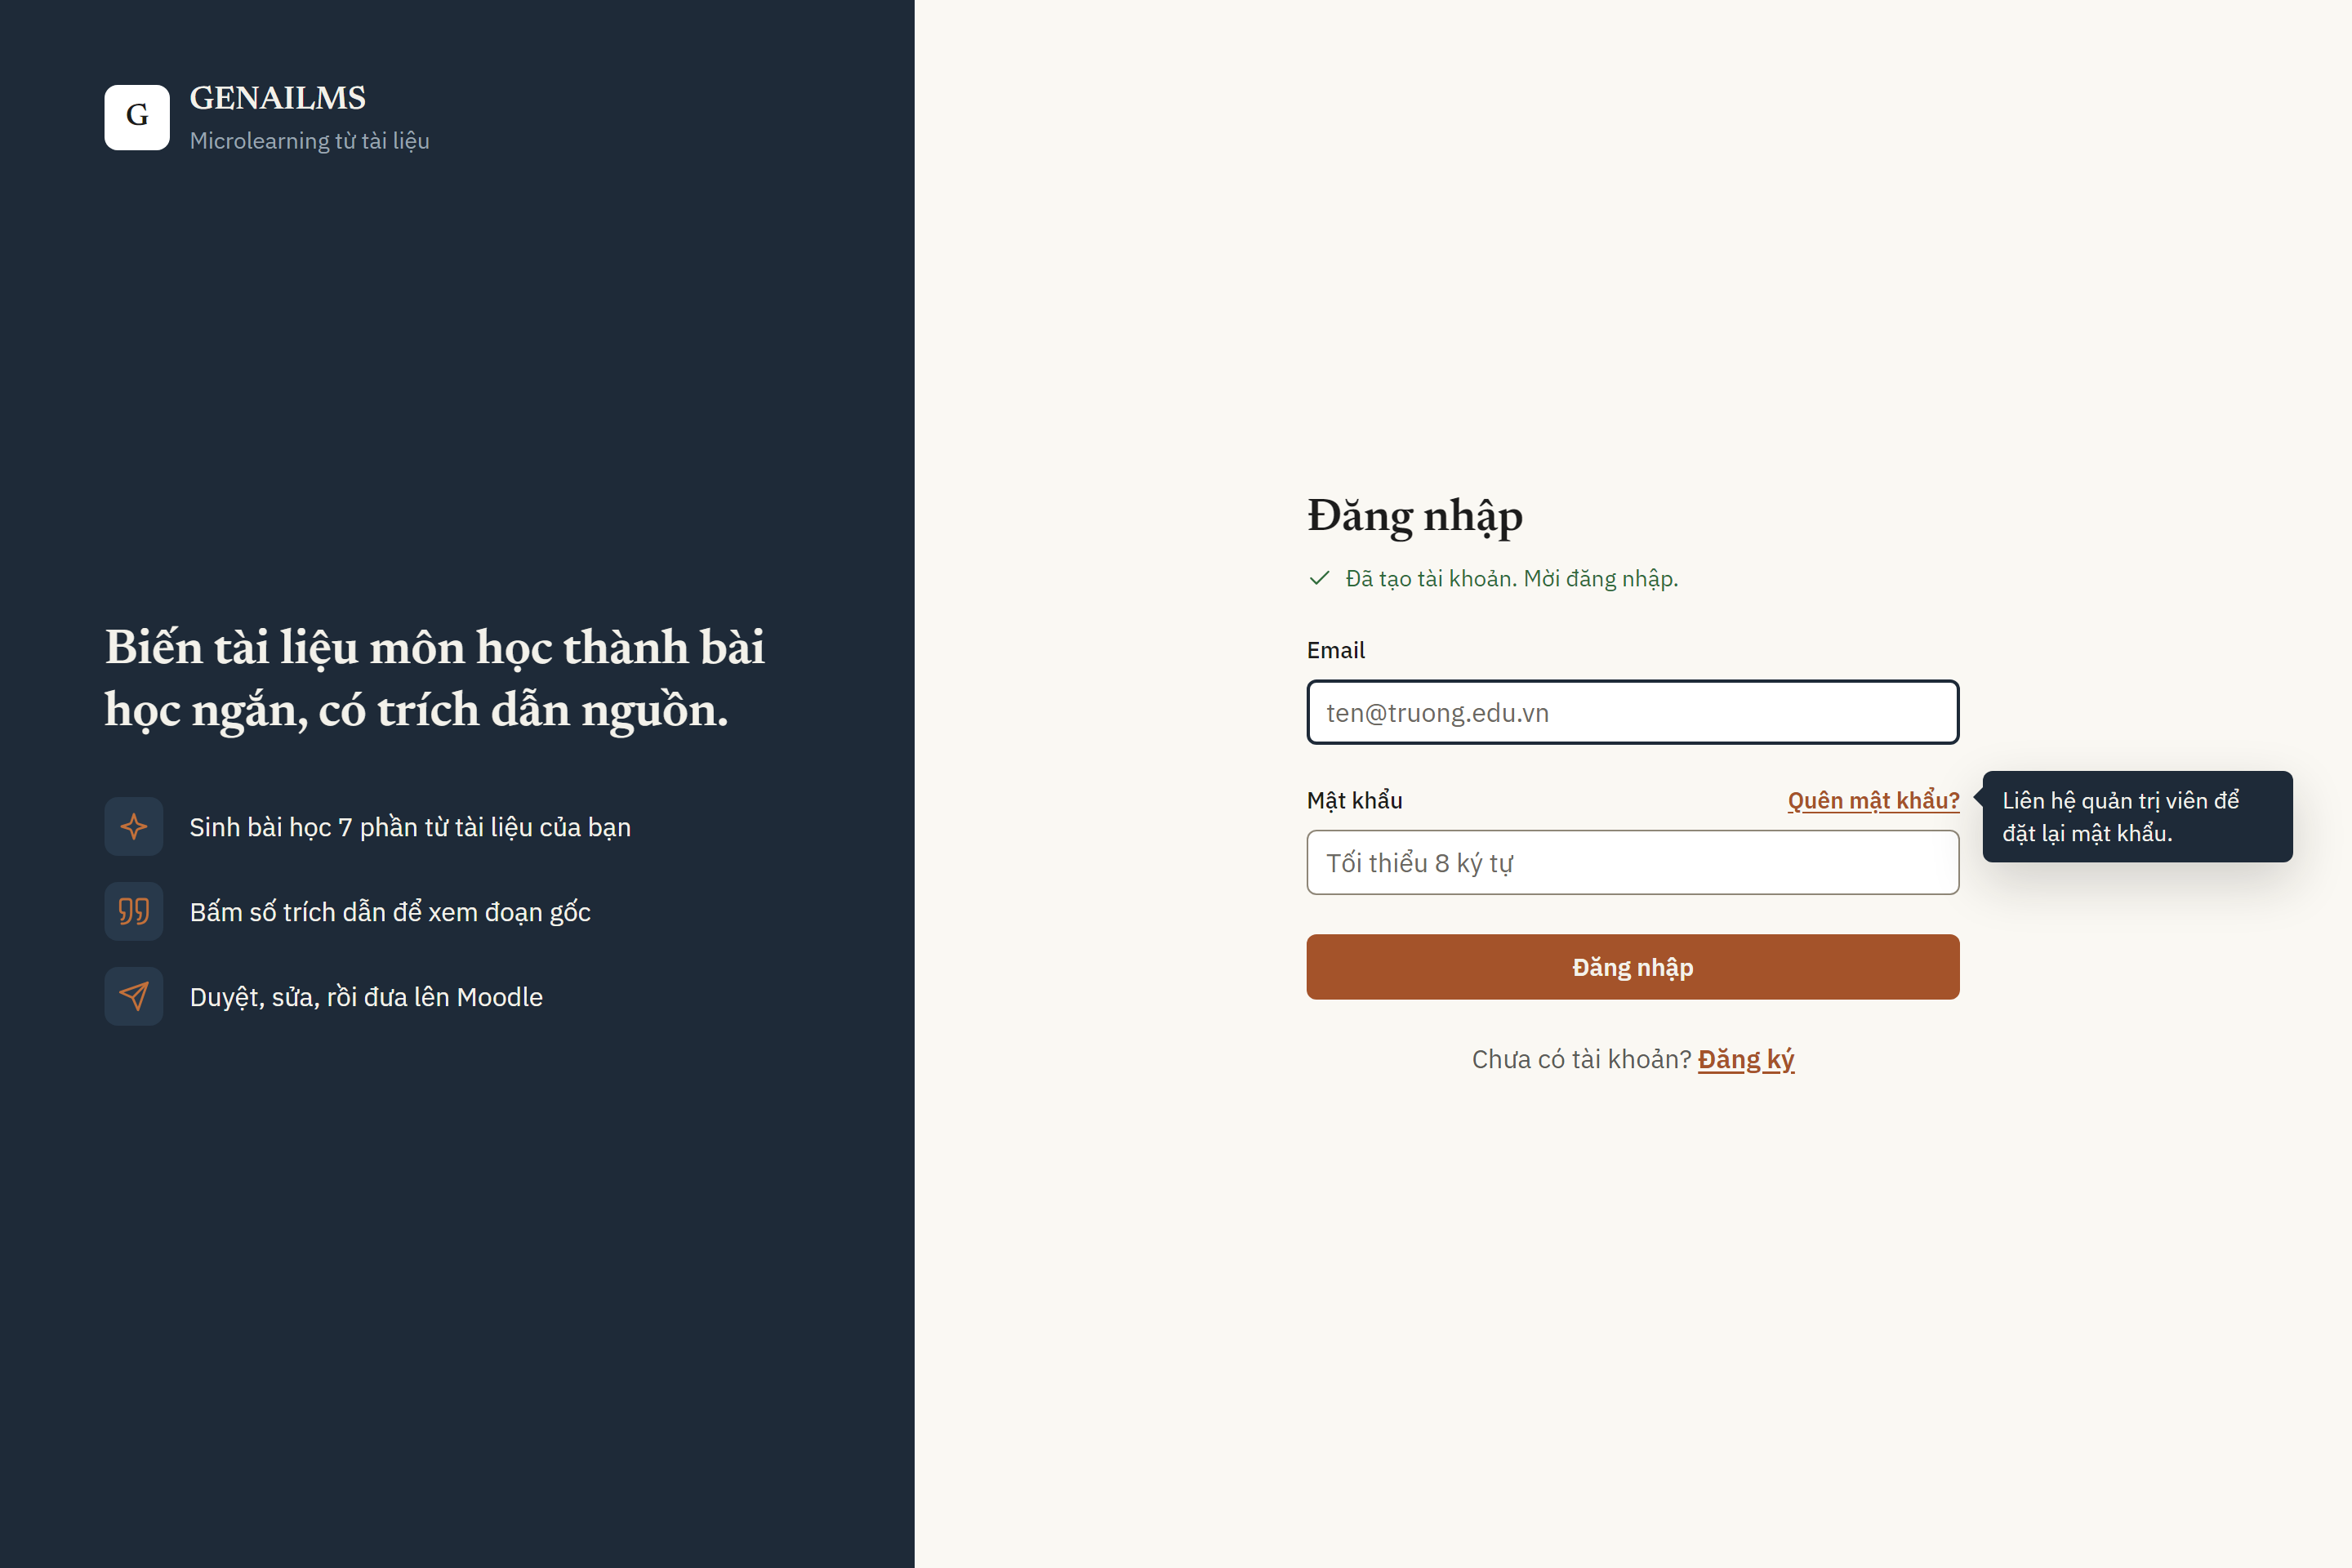
\includegraphics[width=\linewidth,height=.34\textheight,keepaspectratio,viewport={1550 500 2830 1450},clip]{graphics/ui/01-login.png}
\caption{Credential entry and sign-in feedback.}\label{fig:ui-screen-01}
\end{figure}

\needspace{.42\textheight}
Figure~\ref{fig:ui-screen-02} presents registration with persistent labels and repeated-password validation. ``Đăng ký'' means ``Register''; validation remains next to the field that needs correction.
\begin{figure}[H]\centering
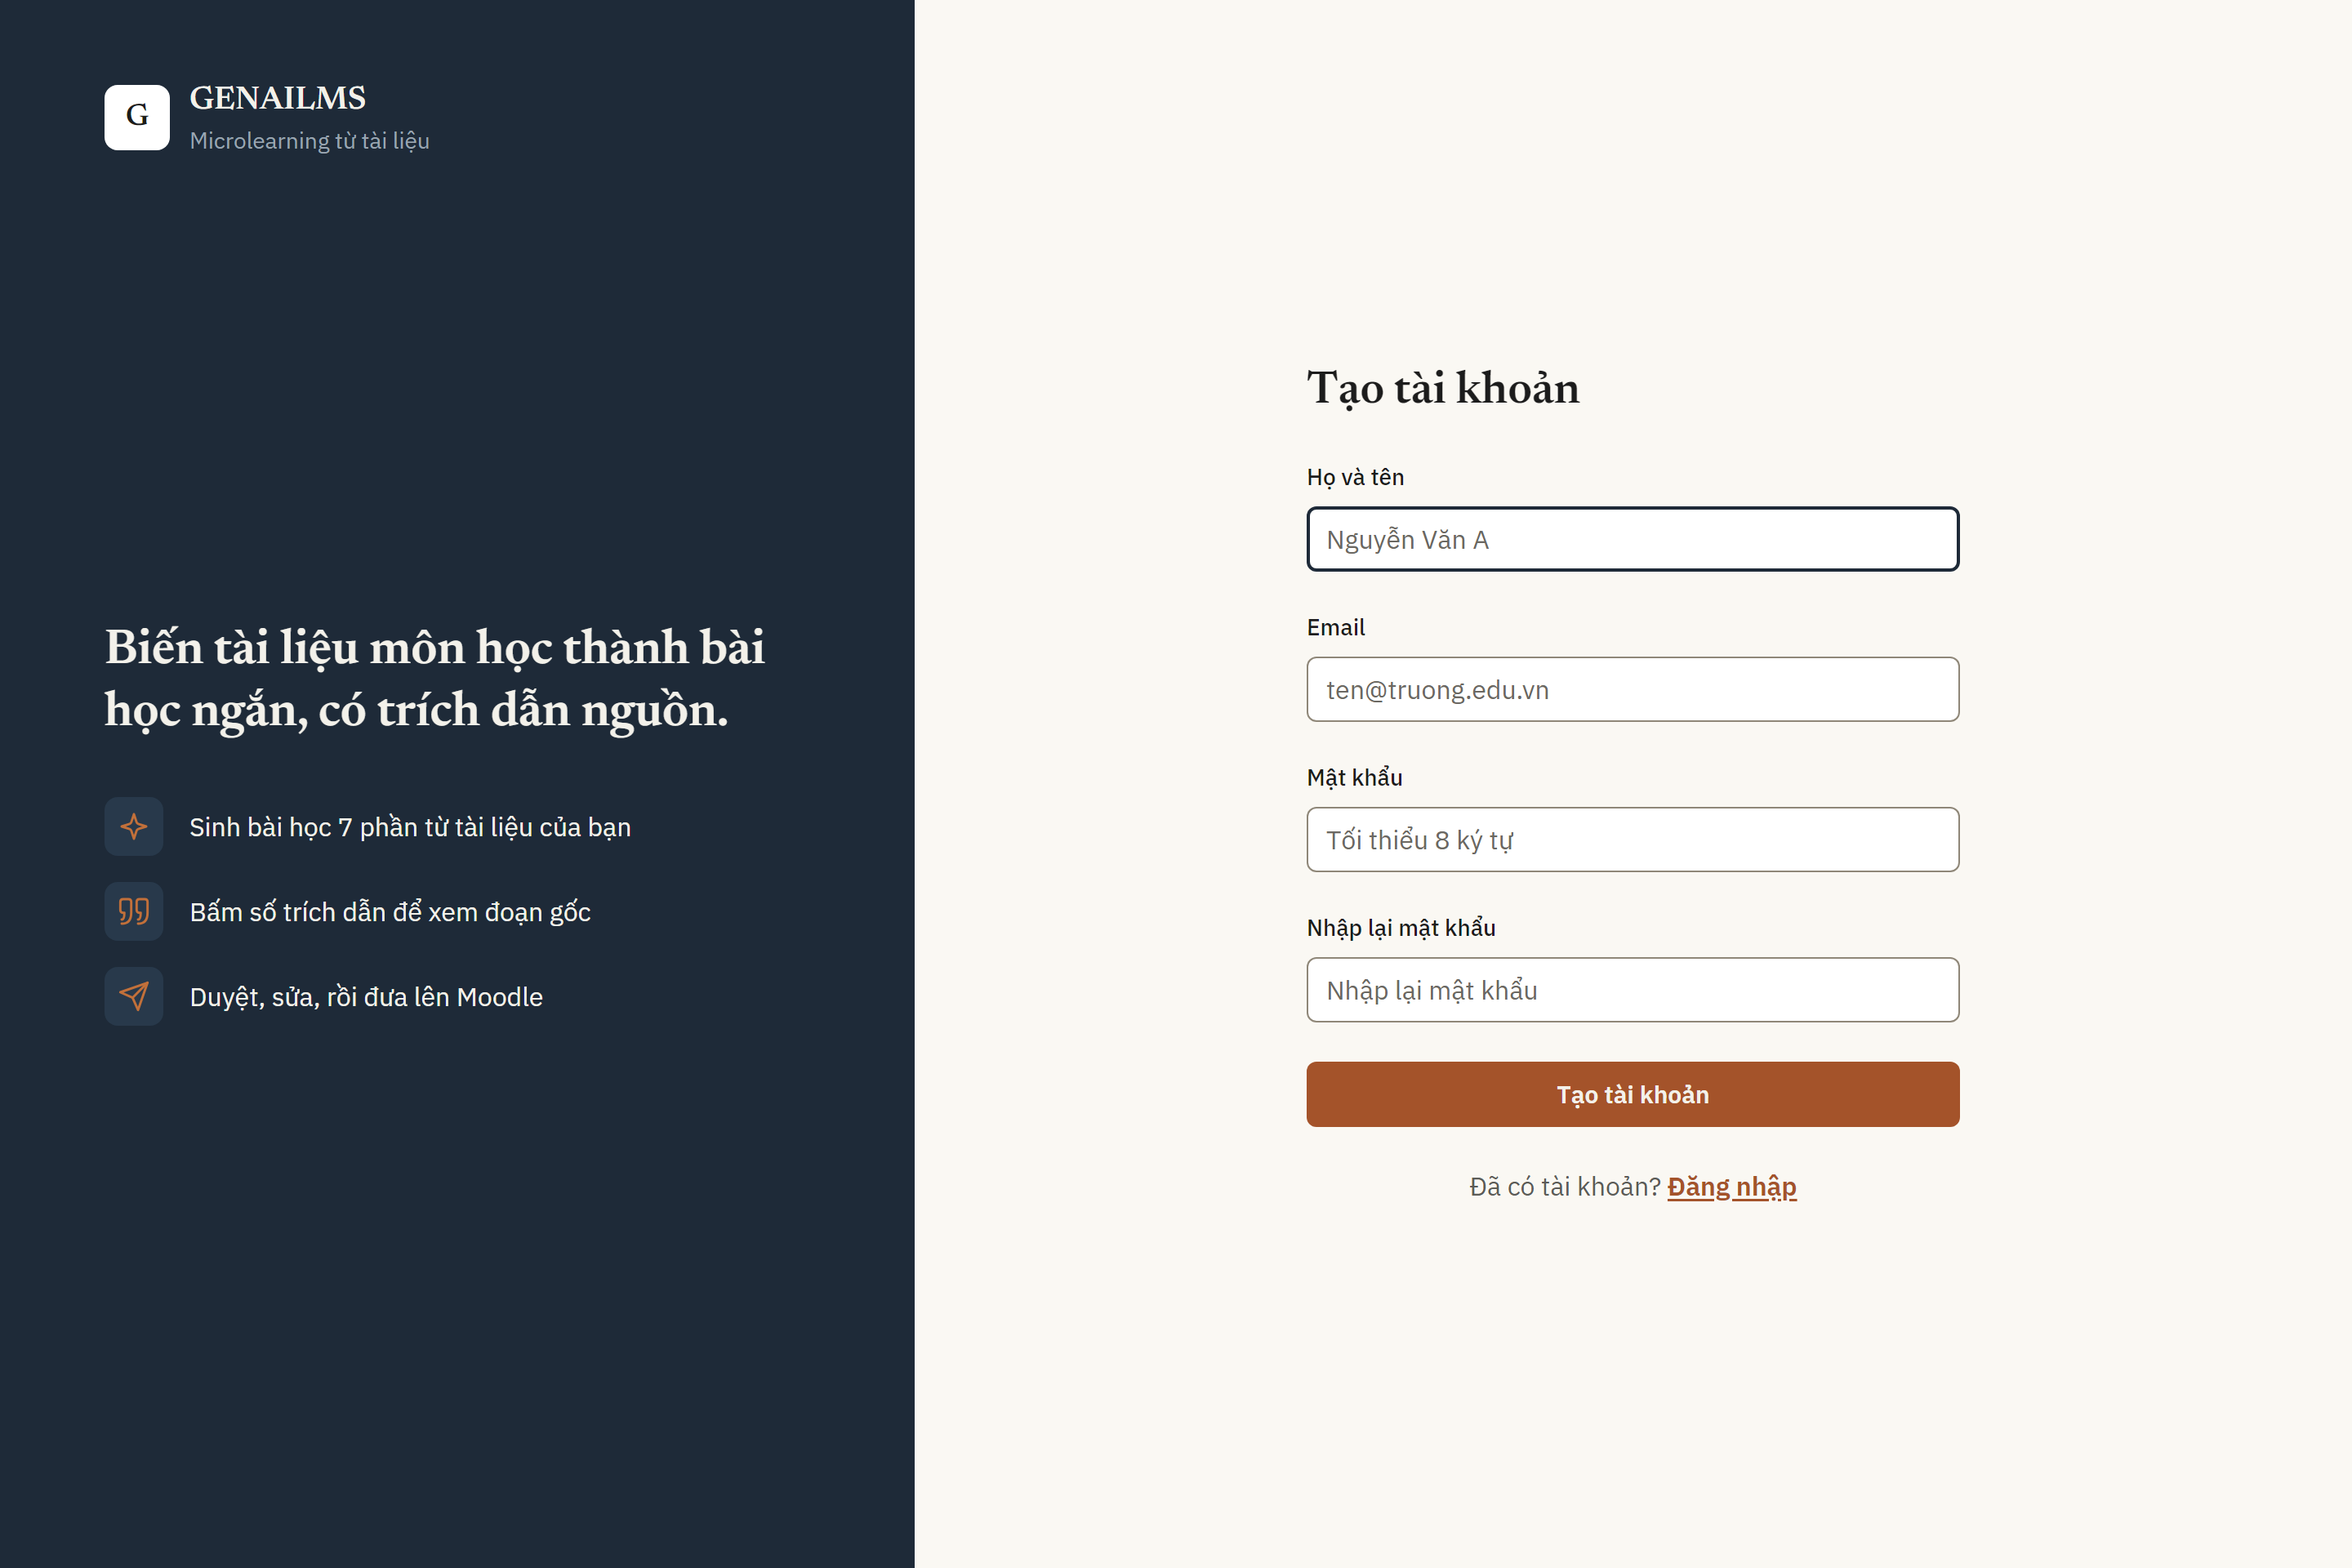
\includegraphics[width=\linewidth,height=.34\textheight,keepaspectratio,viewport={1560 420 2440 1010},clip]{graphics/ui/02-register.png}
\caption{Registration and labelled validation.}\label{fig:ui-screen-02}
\end{figure}

\needspace{.42\textheight}
Figure~\ref{fig:ui-screen-03} organizes the author's owned courses as selectable workspaces. ``Tạo môn học'' means ``Create course''; each card combines the course identity and a compact activity summary.
\begin{figure}[H]\centering
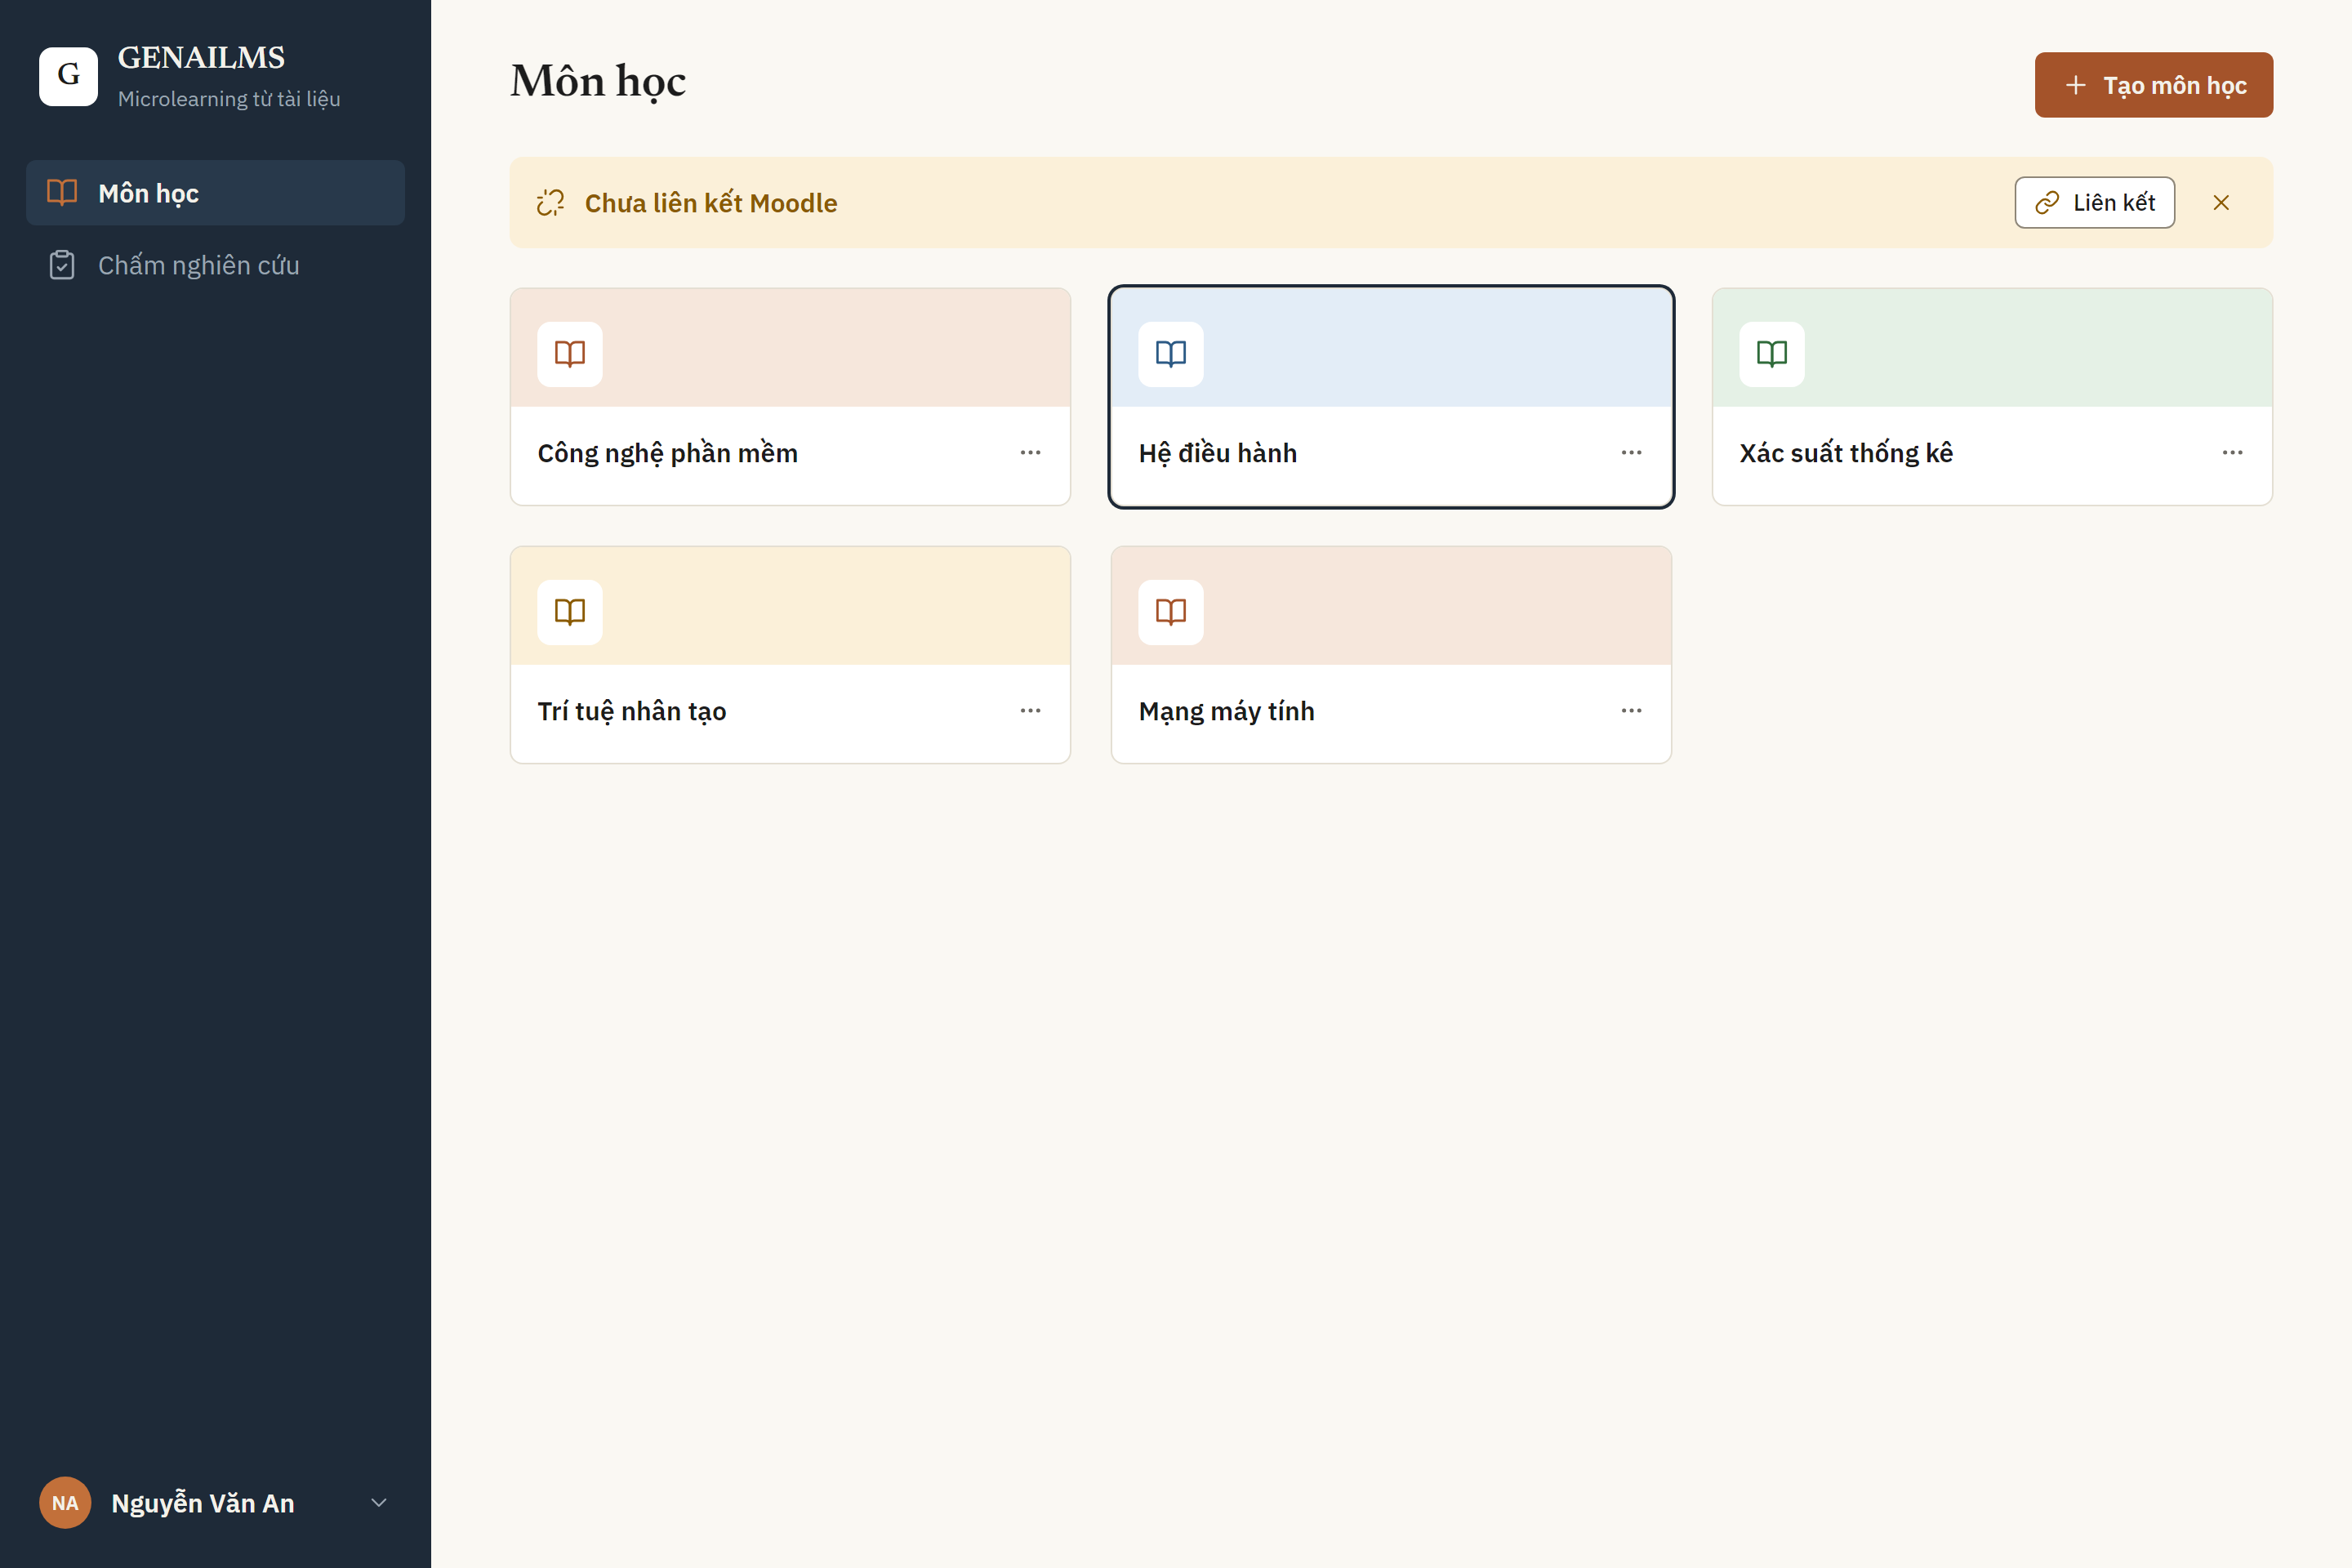
\includegraphics[width=\linewidth,height=.34\textheight,keepaspectratio,viewport={600 960 2070 1600},clip]{graphics/ui/03-course-list-dashboard.png}
\caption{Owned-course workspace selection.}\label{fig:ui-screen-03}
\end{figure}

\needspace{.42\textheight}
The workspace in Figure~\ref{fig:ui-screen-04} combines document status, generation actions and course context. ``Sẵn sàng'' means ``Ready'', while ``Đang xử lý'' means ``Processing''; course Q\&A is entered from this owned-workspace context.
\begin{figure}[H]\centering
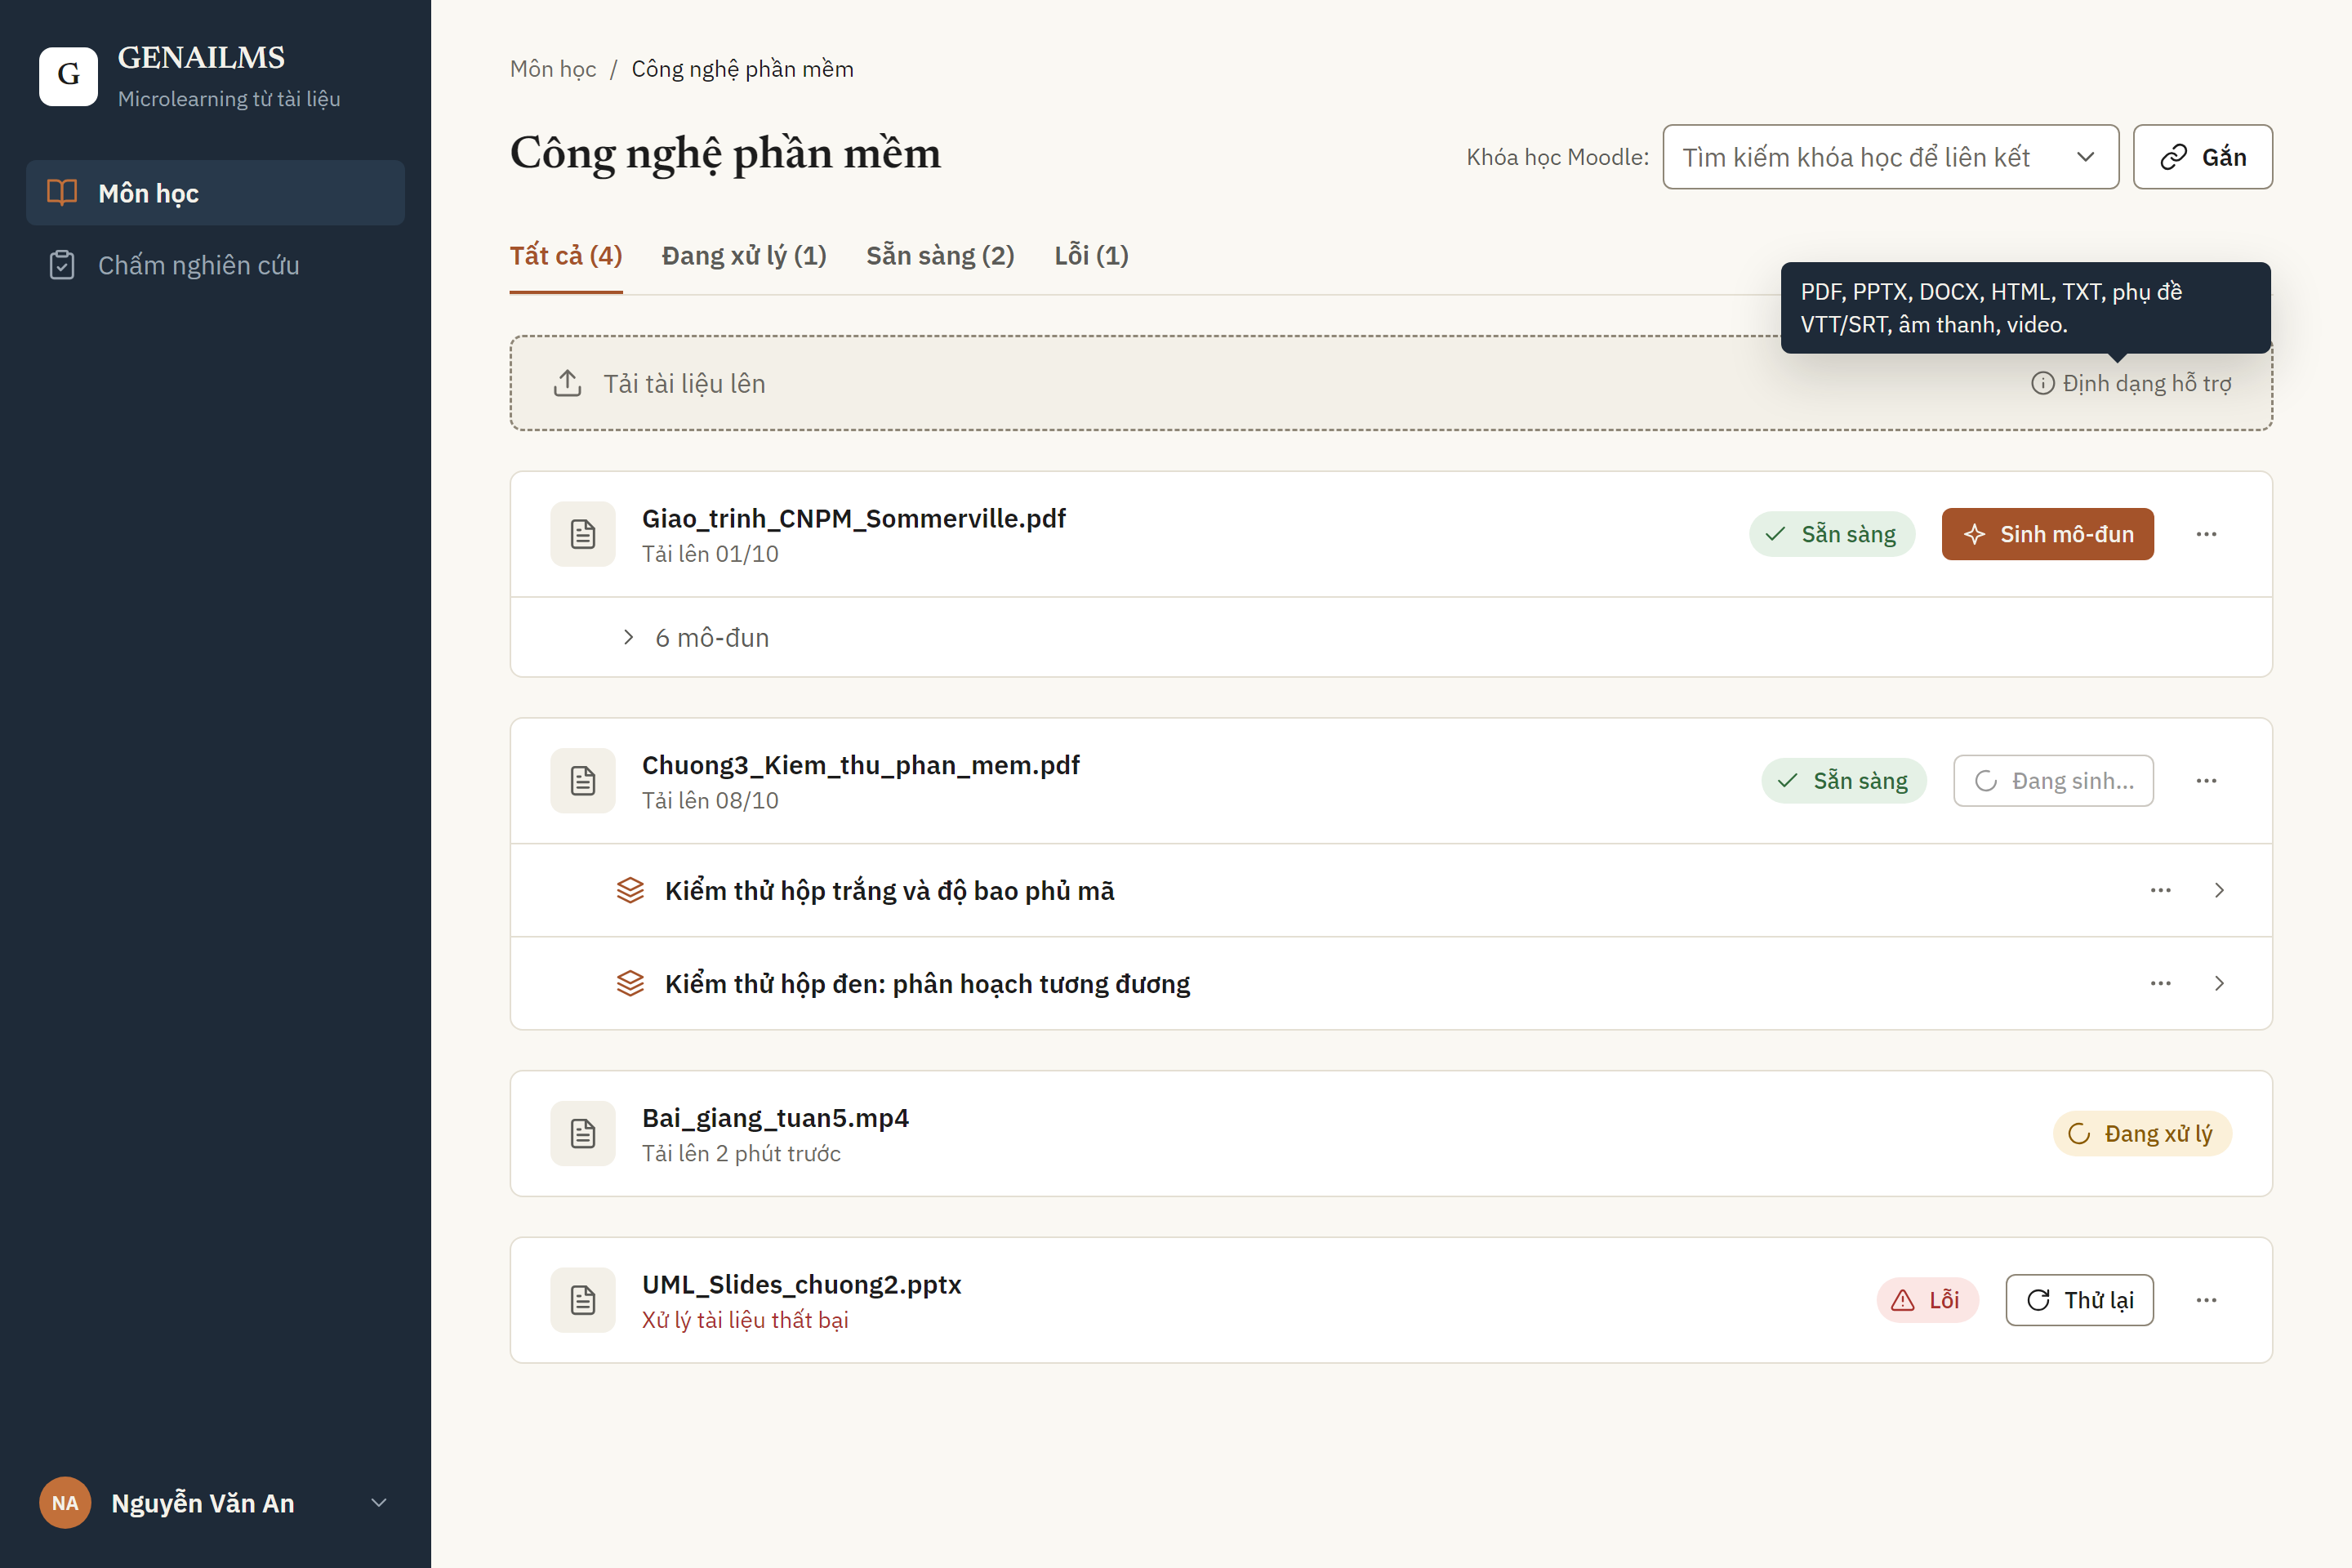
\includegraphics[width=\linewidth,height=.34\textheight,keepaspectratio,viewport={590 600 2820 1800},clip]{graphics/ui/04-course-detail.png}
\caption{Course documents and processing feedback.}\label{fig:ui-screen-04}
\end{figure}

\needspace{.42\textheight}
Figure~\ref{fig:ui-screen-05} asks the author to confirm a model, output language and additional guidance before generation. ``Mặc định'' means ``Default'' and ``Sinh mô-đun'' means ``Generate module''; the saved preference preselects the model without preventing a one-request override.
\begin{figure}[H]\centering
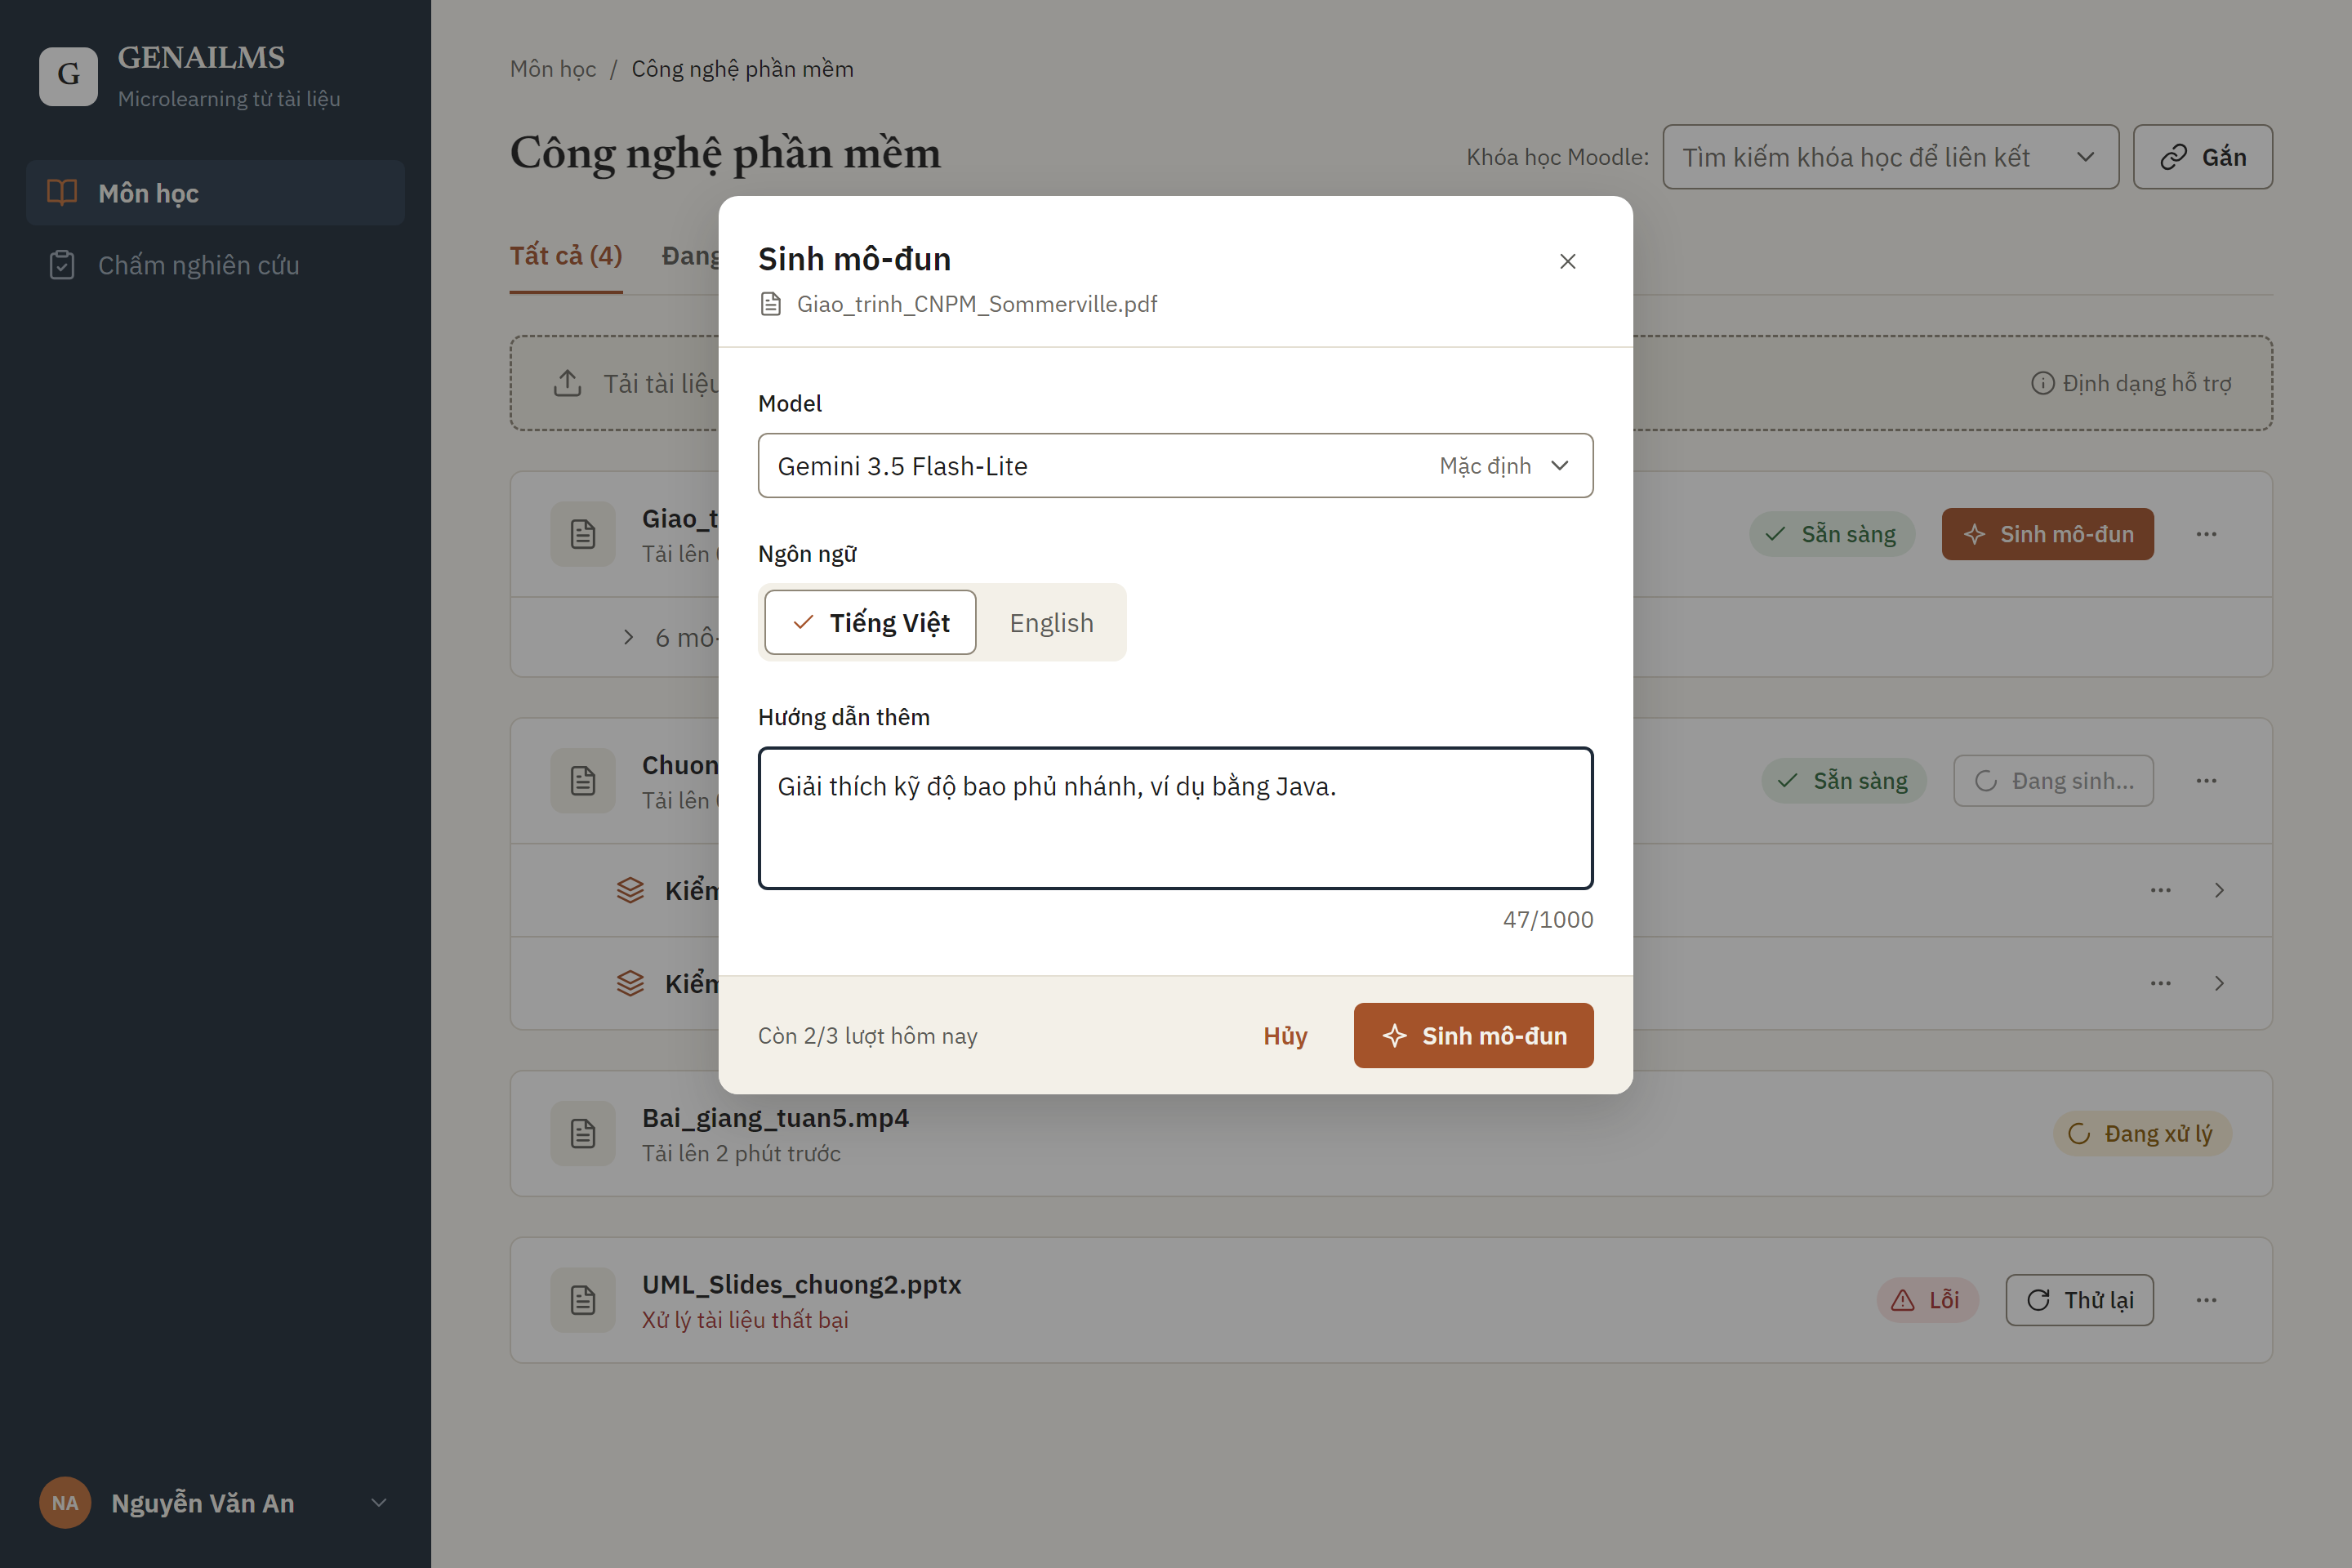
\includegraphics[width=\linewidth,height=.42\textheight,keepaspectratio,viewport={900 585 1980 1510},clip]{graphics/ui/05-generate-module-dialog.png}
\caption{Generation choices before submitting a job.}\label{fig:ui-screen-05}
\end{figure}

\needspace{.42\textheight}
Figure~\ref{fig:ui-screen-06} enlarges the highlighted claim and its source panel as two views of the same screen. ``Nguồn'' means ``Sources'' and ``Khớp'' means ``Matched''; an unresolved source remains visible for review rather than receiving a fabricated match.
\begin{figure}[H]\centering
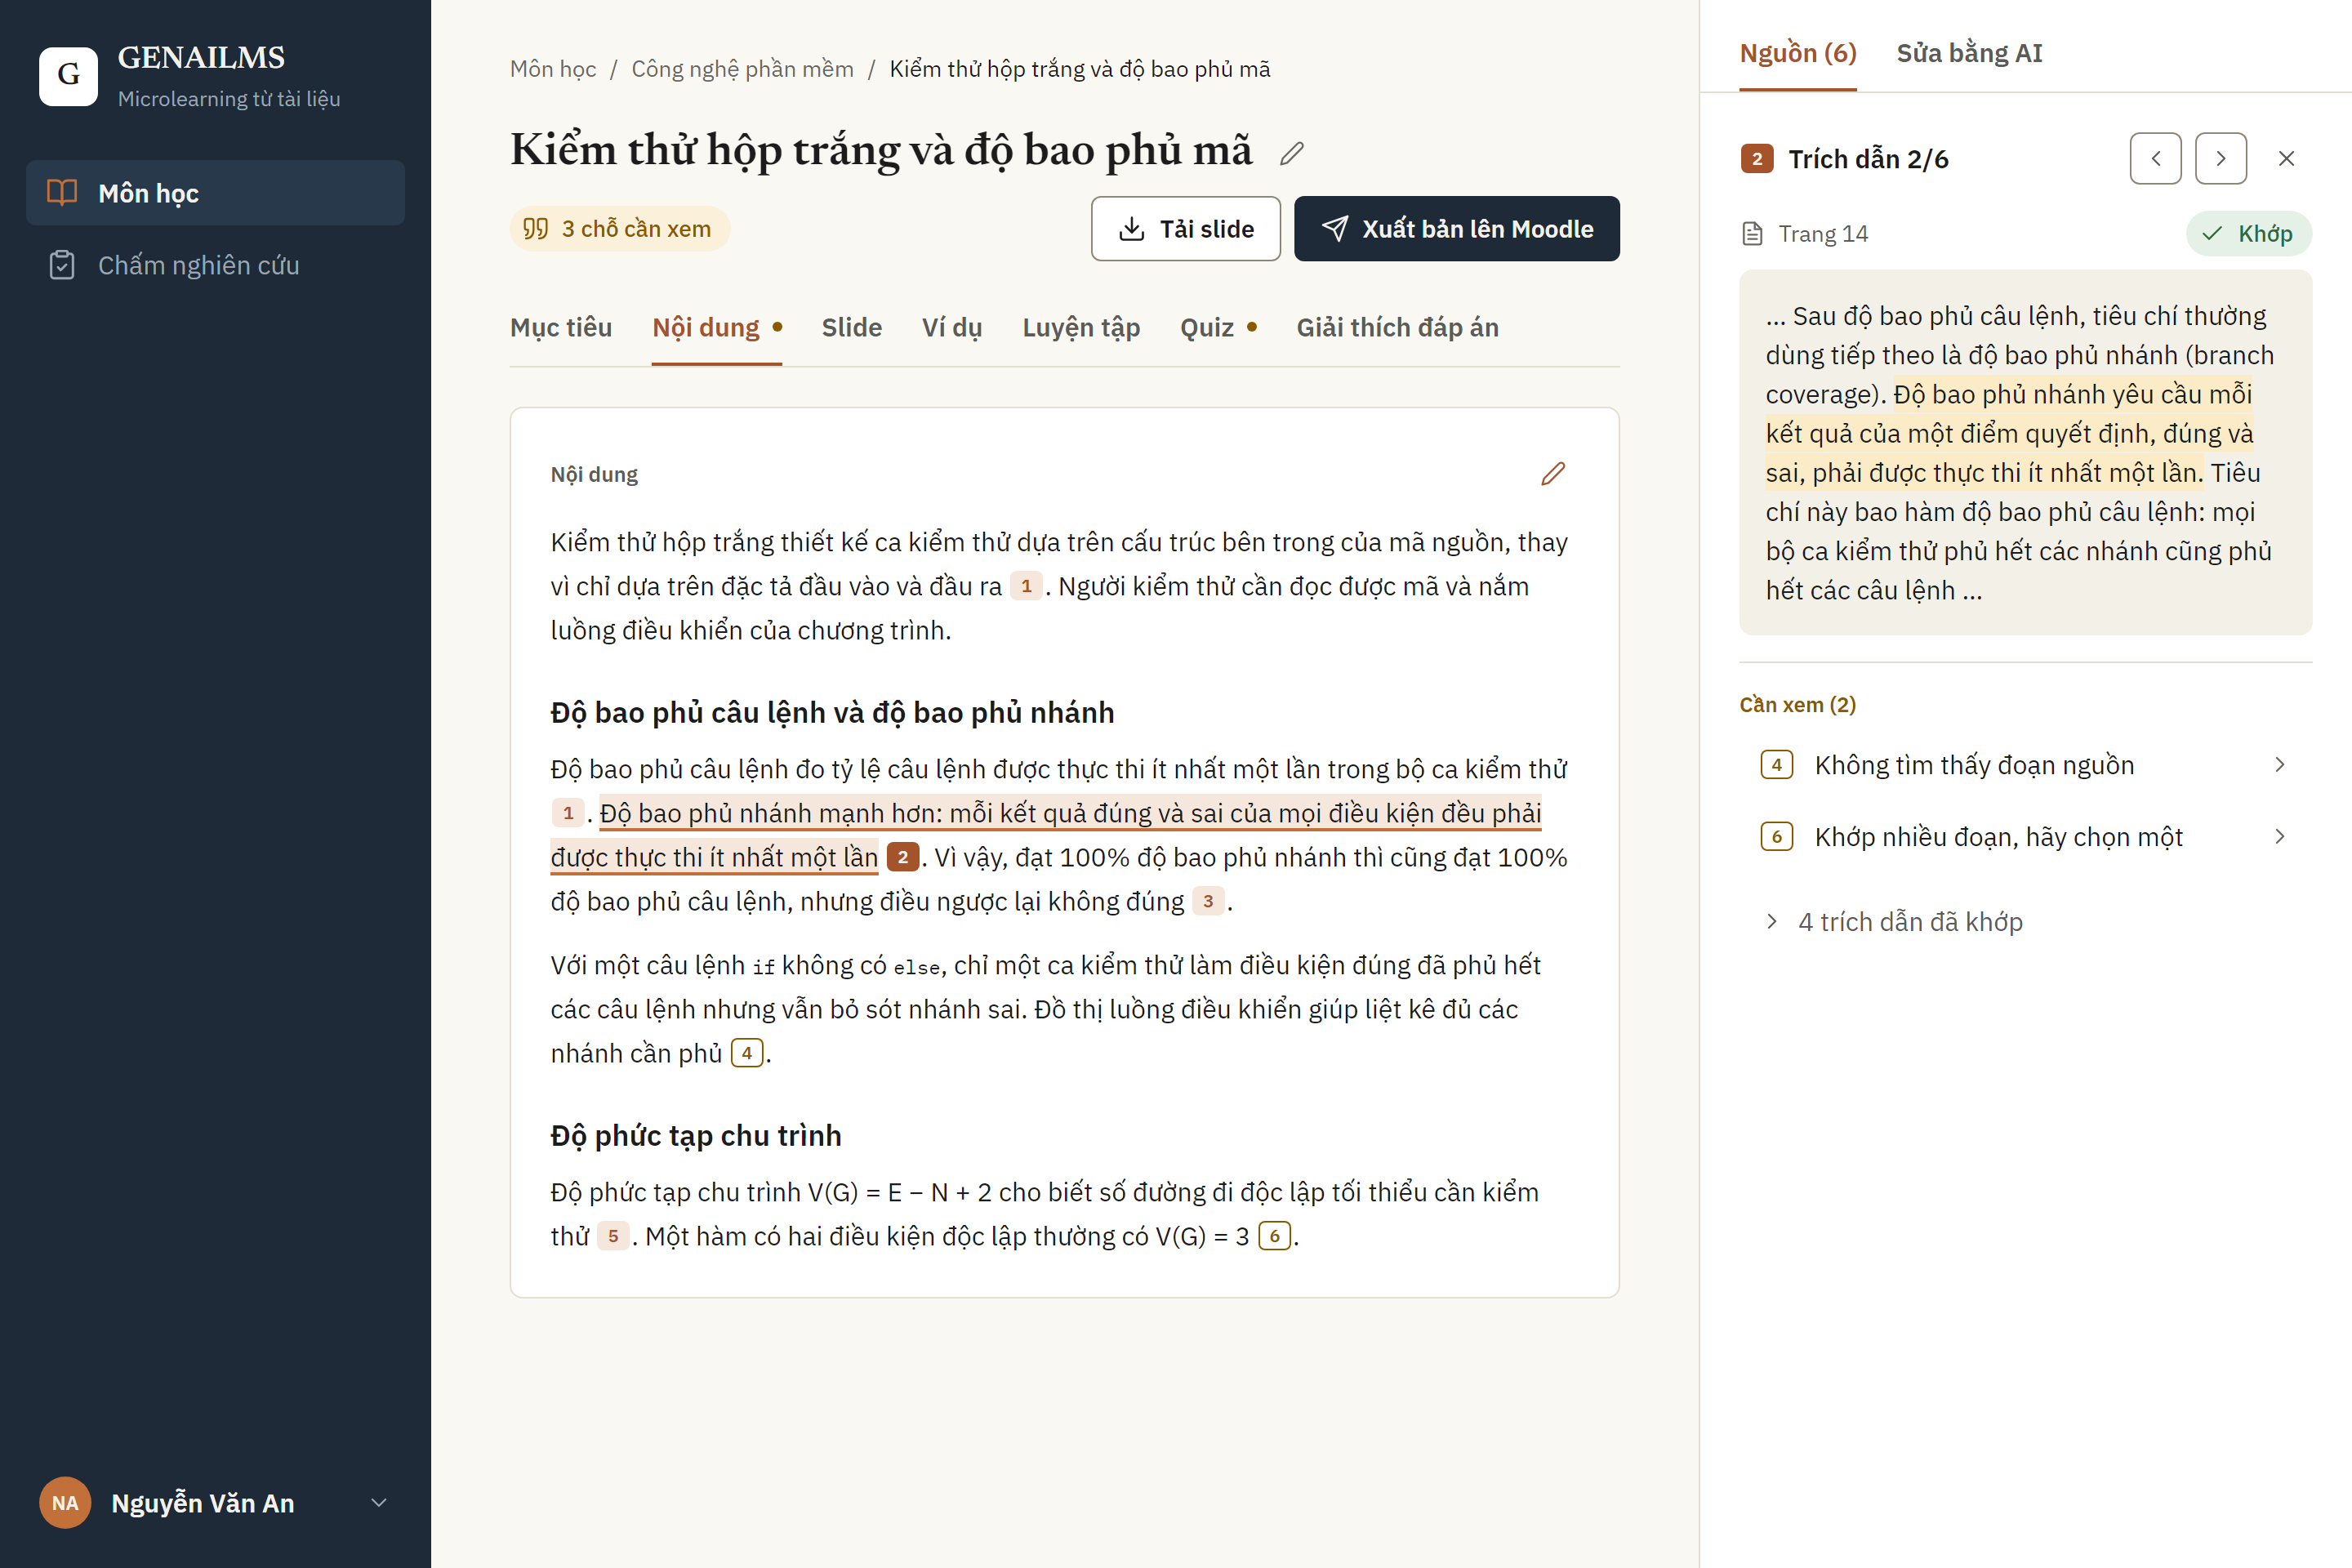
\includegraphics[width=\linewidth,height=.27\textheight,keepaspectratio,viewport={650 570 2000 1150},clip]{graphics/ui/06-module-editor-citations.png}\par\smallskip
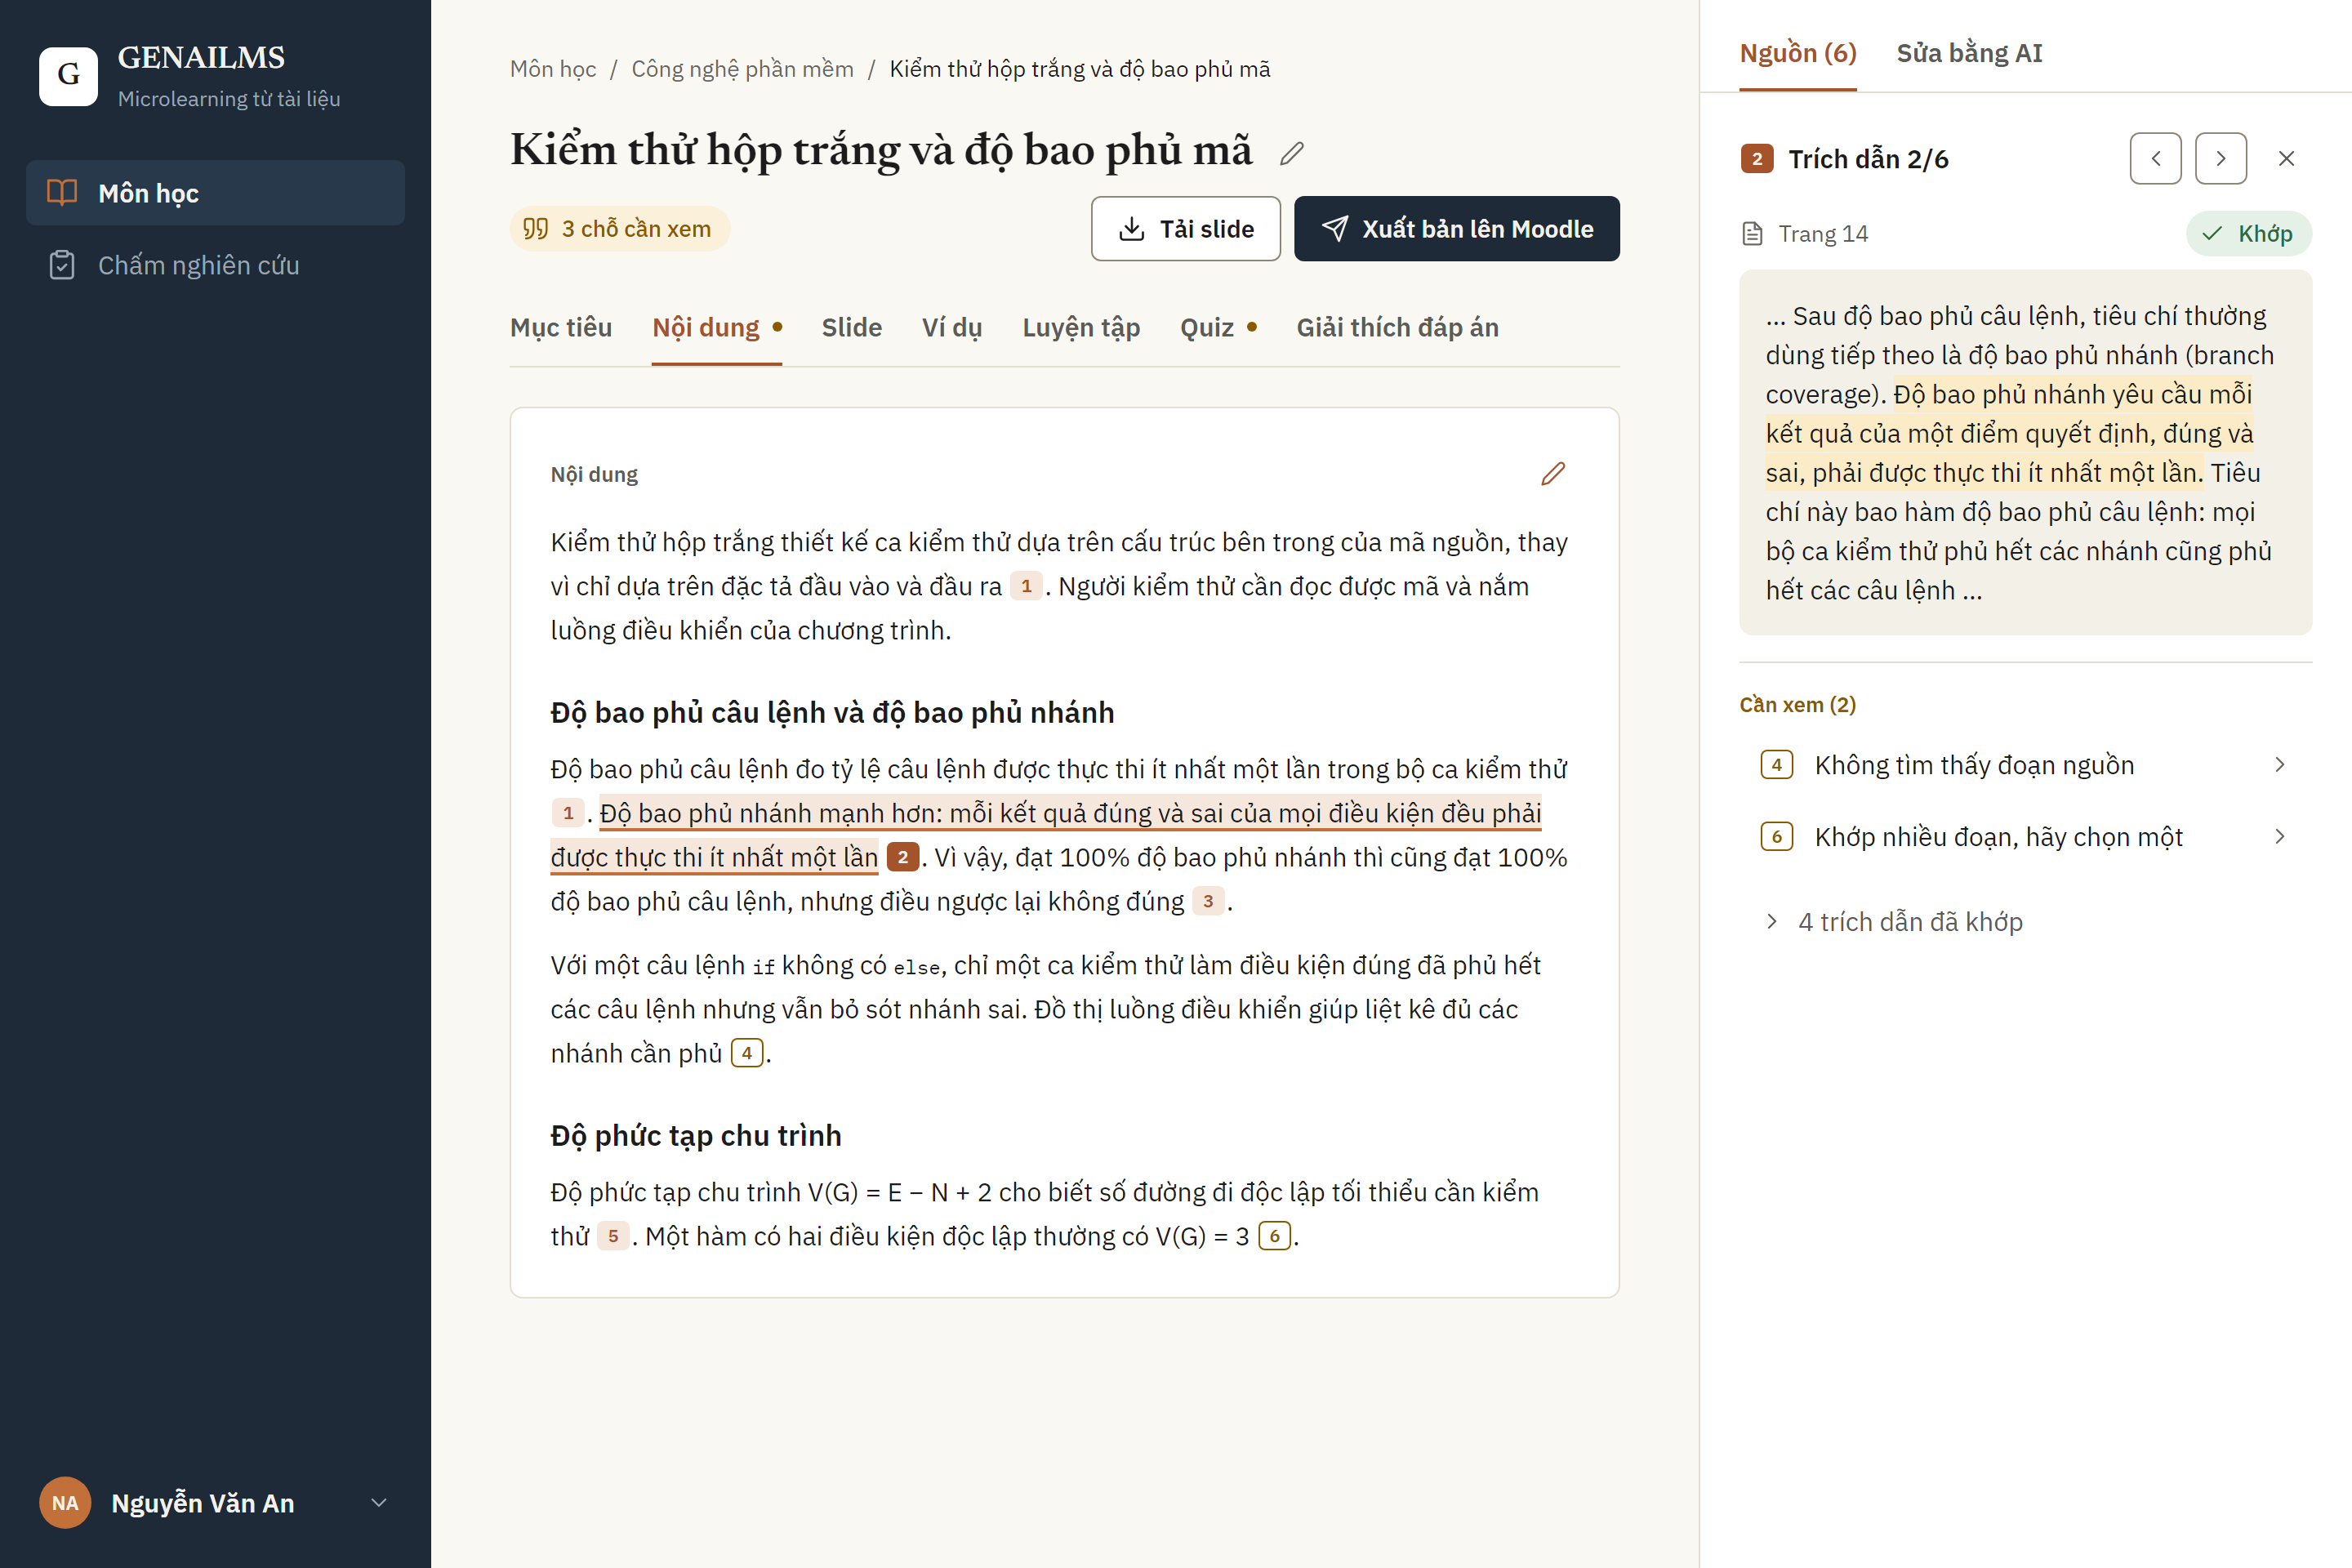
\includegraphics[width=\linewidth,height=.27\textheight,keepaspectratio,viewport={2080 1120 2850 1800},clip]{graphics/ui/06-module-editor-citations.png}
\caption{Claim marker and corresponding physical source passage.}\label{fig:ui-screen-06}
\end{figure}

\needspace{.42\textheight}
The contextual panel in Figure~\ref{fig:ui-screen-07} accepts a component-edit request while retaining the lesson context. ``Sửa bằng AI'' means ``Edit with AI''; accepting an edit follows the same validation and original-preservation contract as a manual change.
\begin{figure}[H]\centering
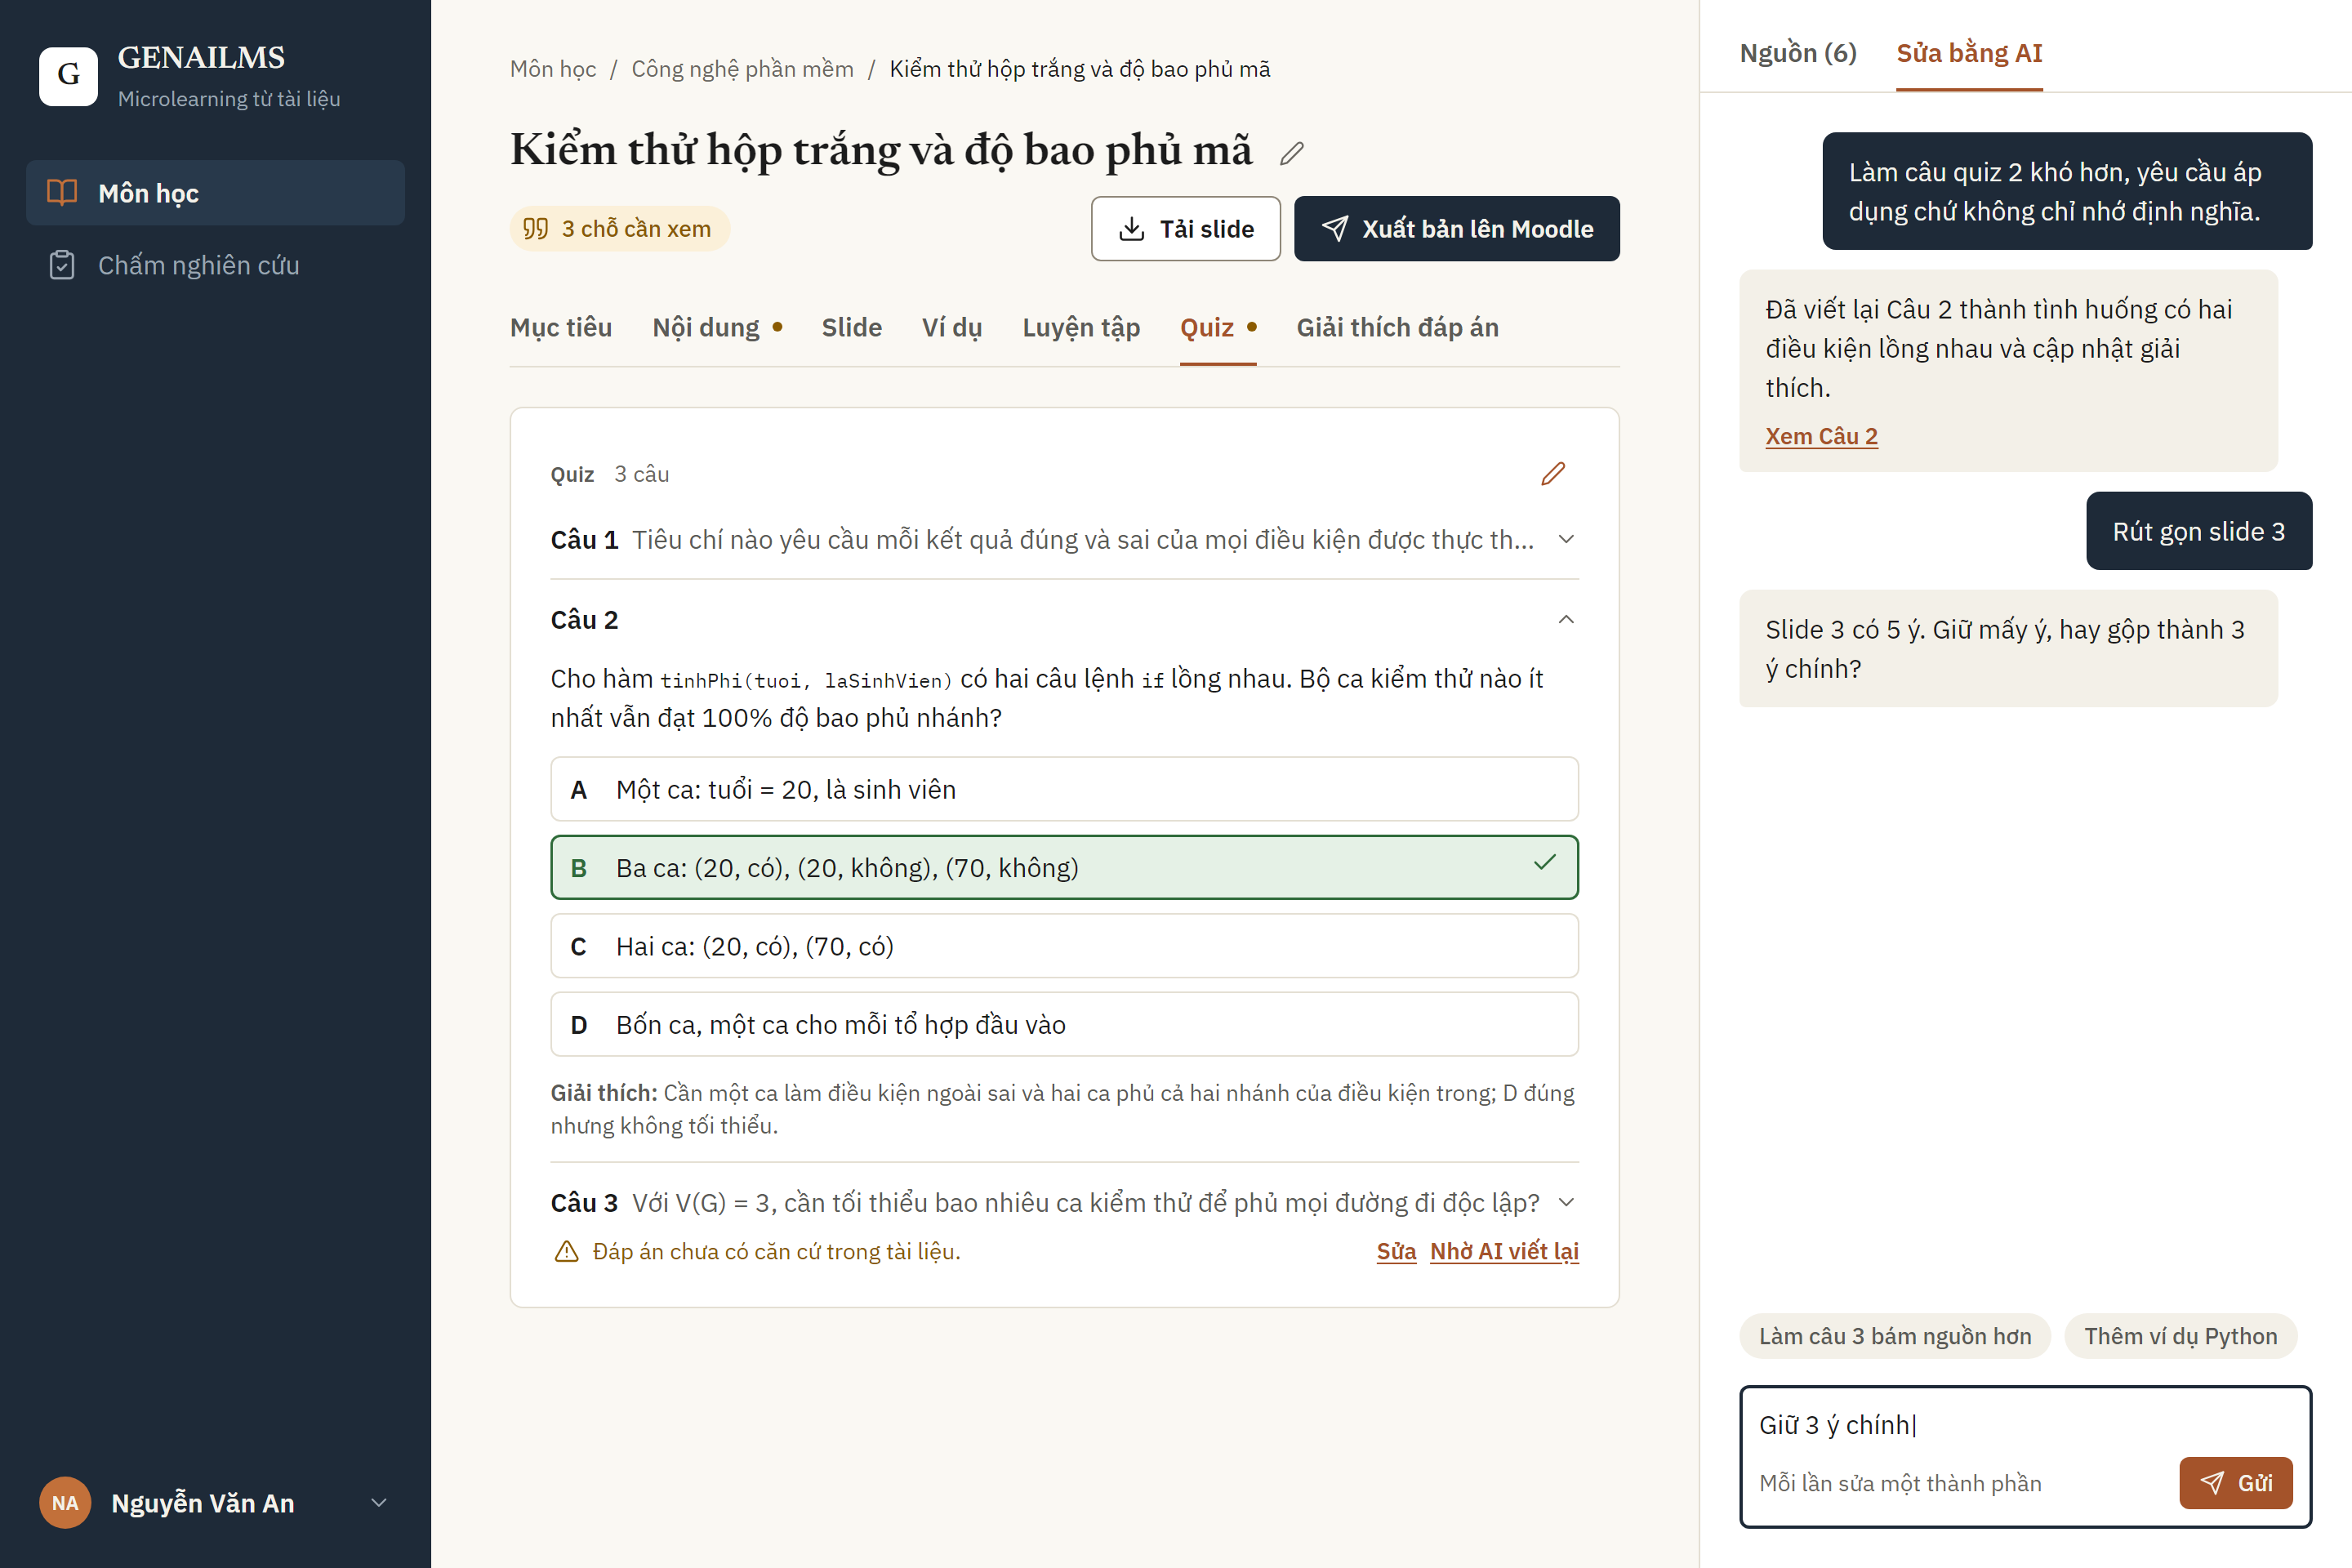
\includegraphics[width=\linewidth,height=.34\textheight,keepaspectratio,viewport={2100 1320 2850 1780},clip]{graphics/ui/07-module-editor-chat-edit.png}
\caption{Contextual editing request and response.}\label{fig:ui-screen-07}
\end{figure}

\needspace{.42\textheight}
Figure~\ref{fig:ui-screen-08} makes the target course/section and activity selection visible before publication. ``Xuất bản lên Moodle'' means ``Publish to Moodle''; the explicit confirmation reduces accidental publication to a remembered destination.
\begin{figure}[H]\centering
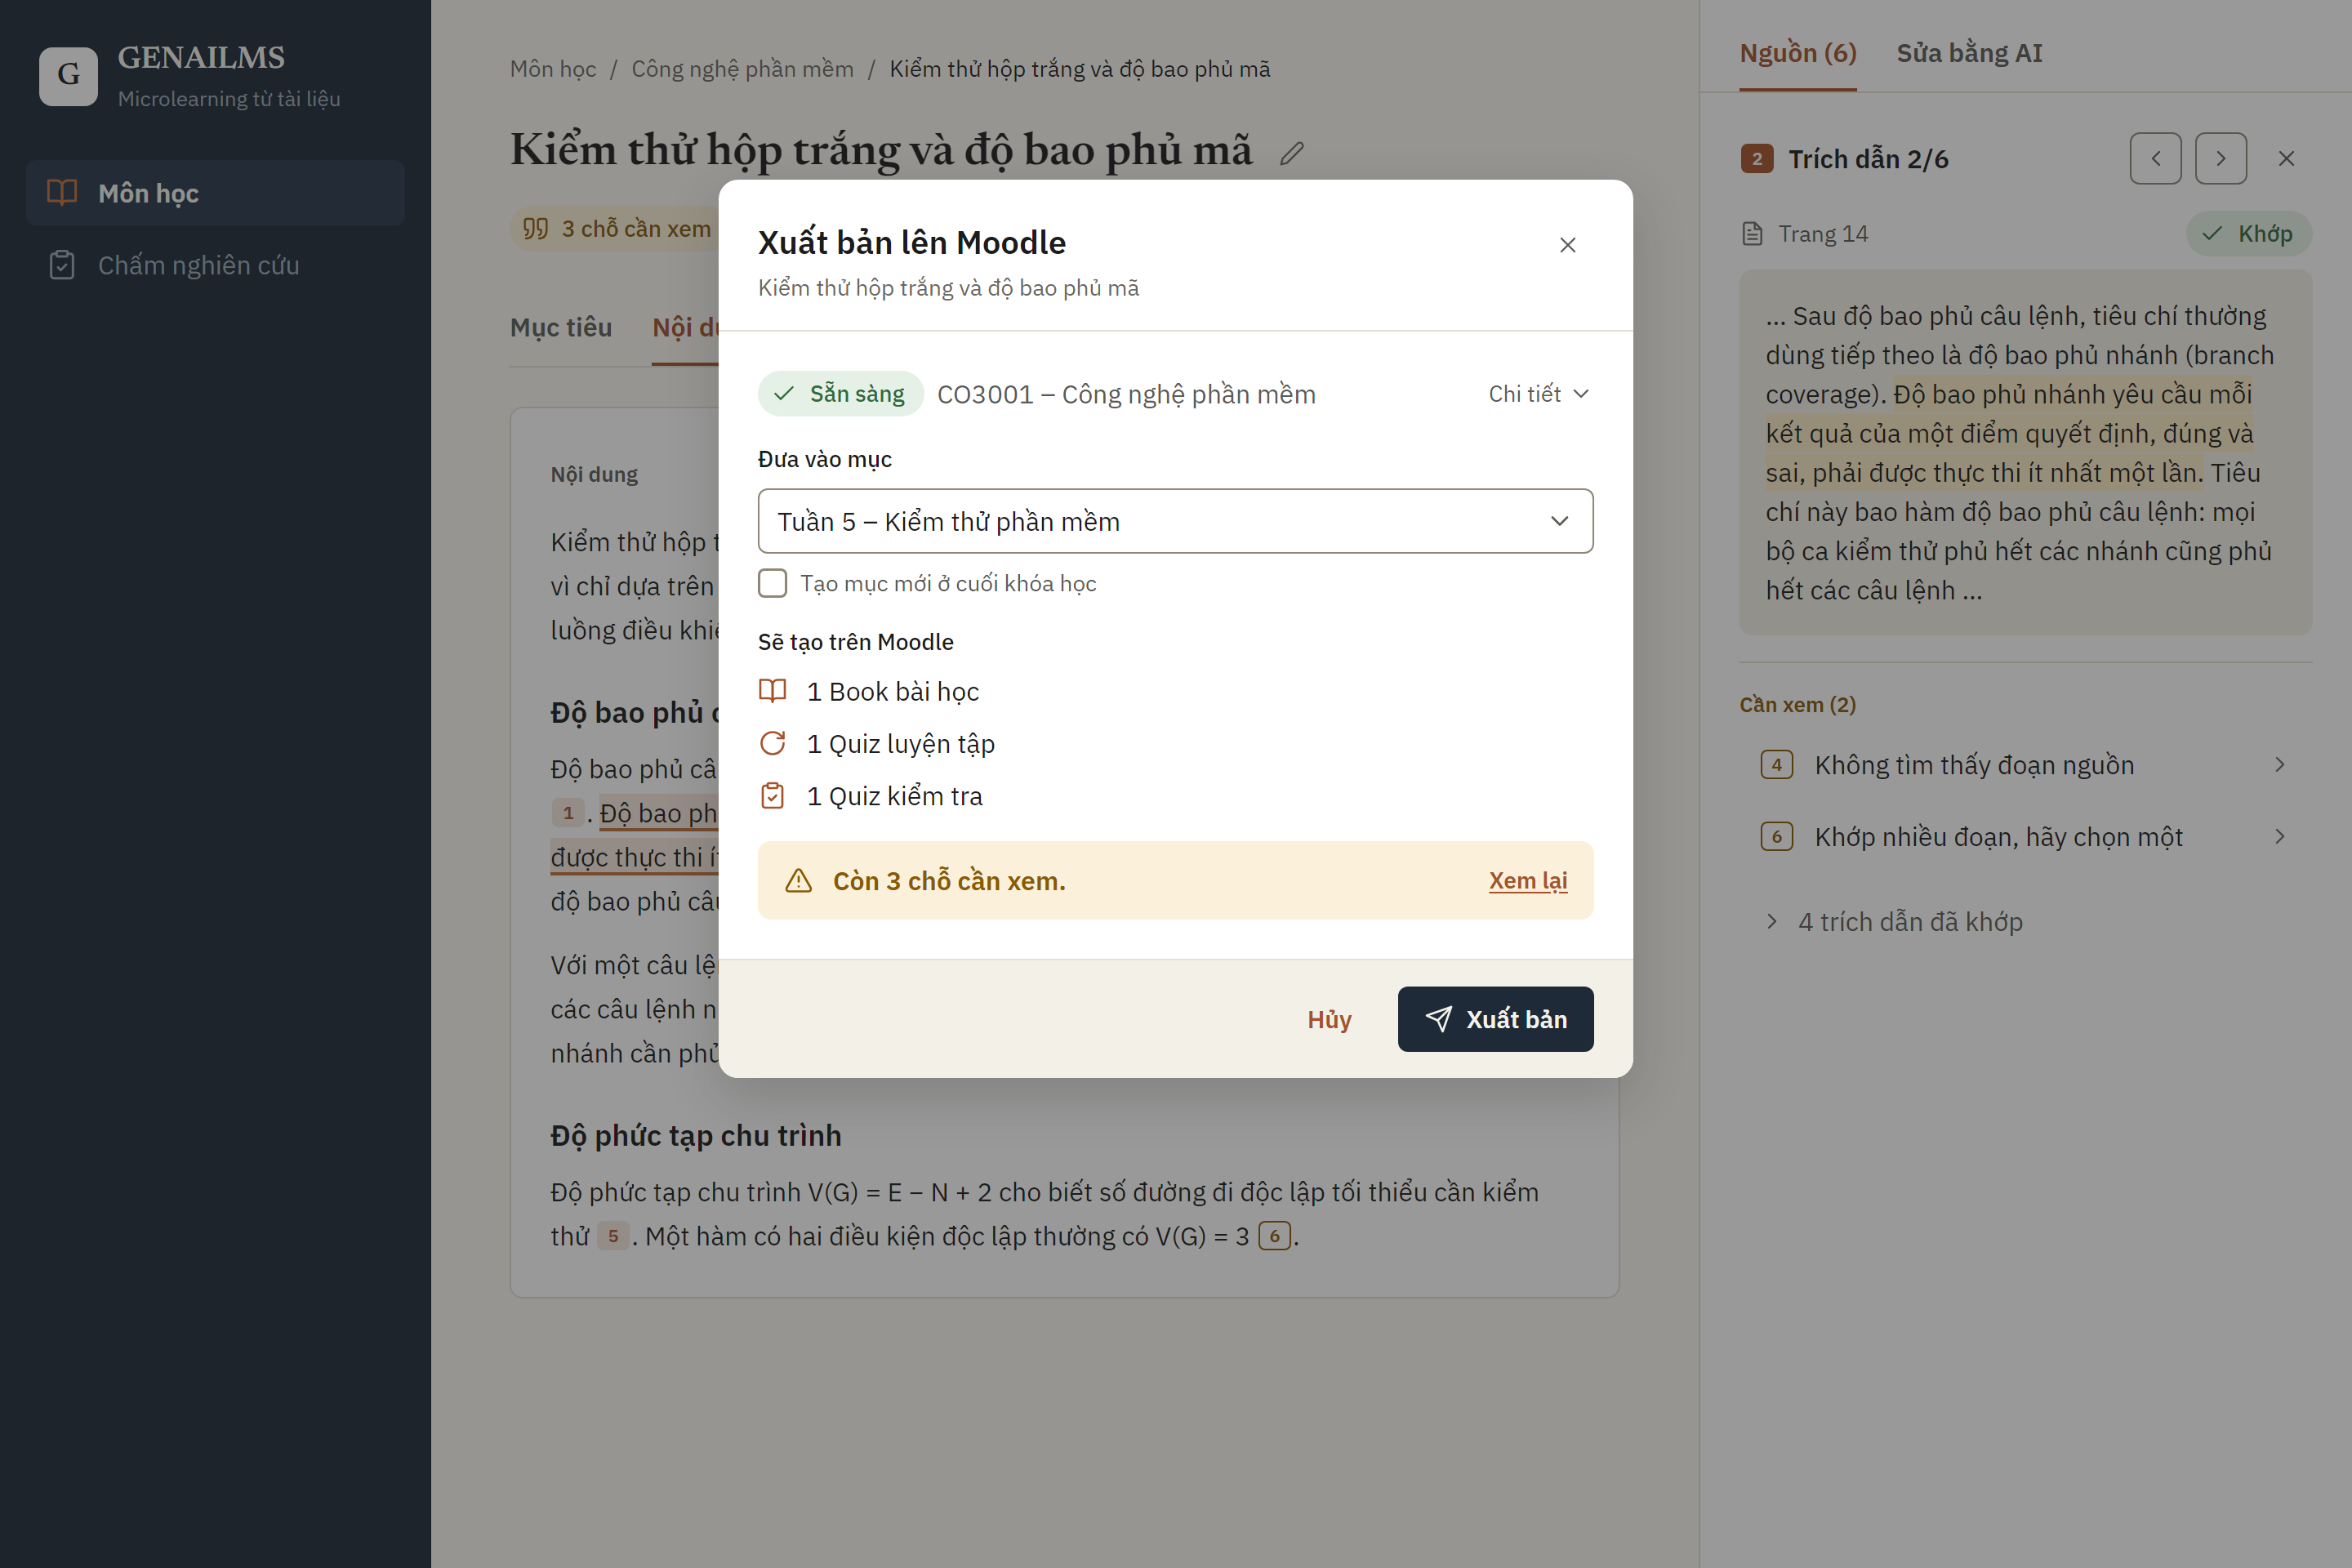
\includegraphics[width=\linewidth,height=.42\textheight,keepaspectratio,viewport={900 600 1980 1510},clip]{graphics/ui/08-publish-to-moodle.png}
\caption{Publication destination and activity review.}\label{fig:ui-screen-08}
\end{figure}

\needspace{.42\textheight}
Figure~\ref{fig:ui-screen-09} highlights pending identity confirmation and its next action. Account linking and course permission remain separate states; subsequent publication verifies the target-course capabilities without exposing account existence through the generic link-request response.
\begin{figure}[H]\centering
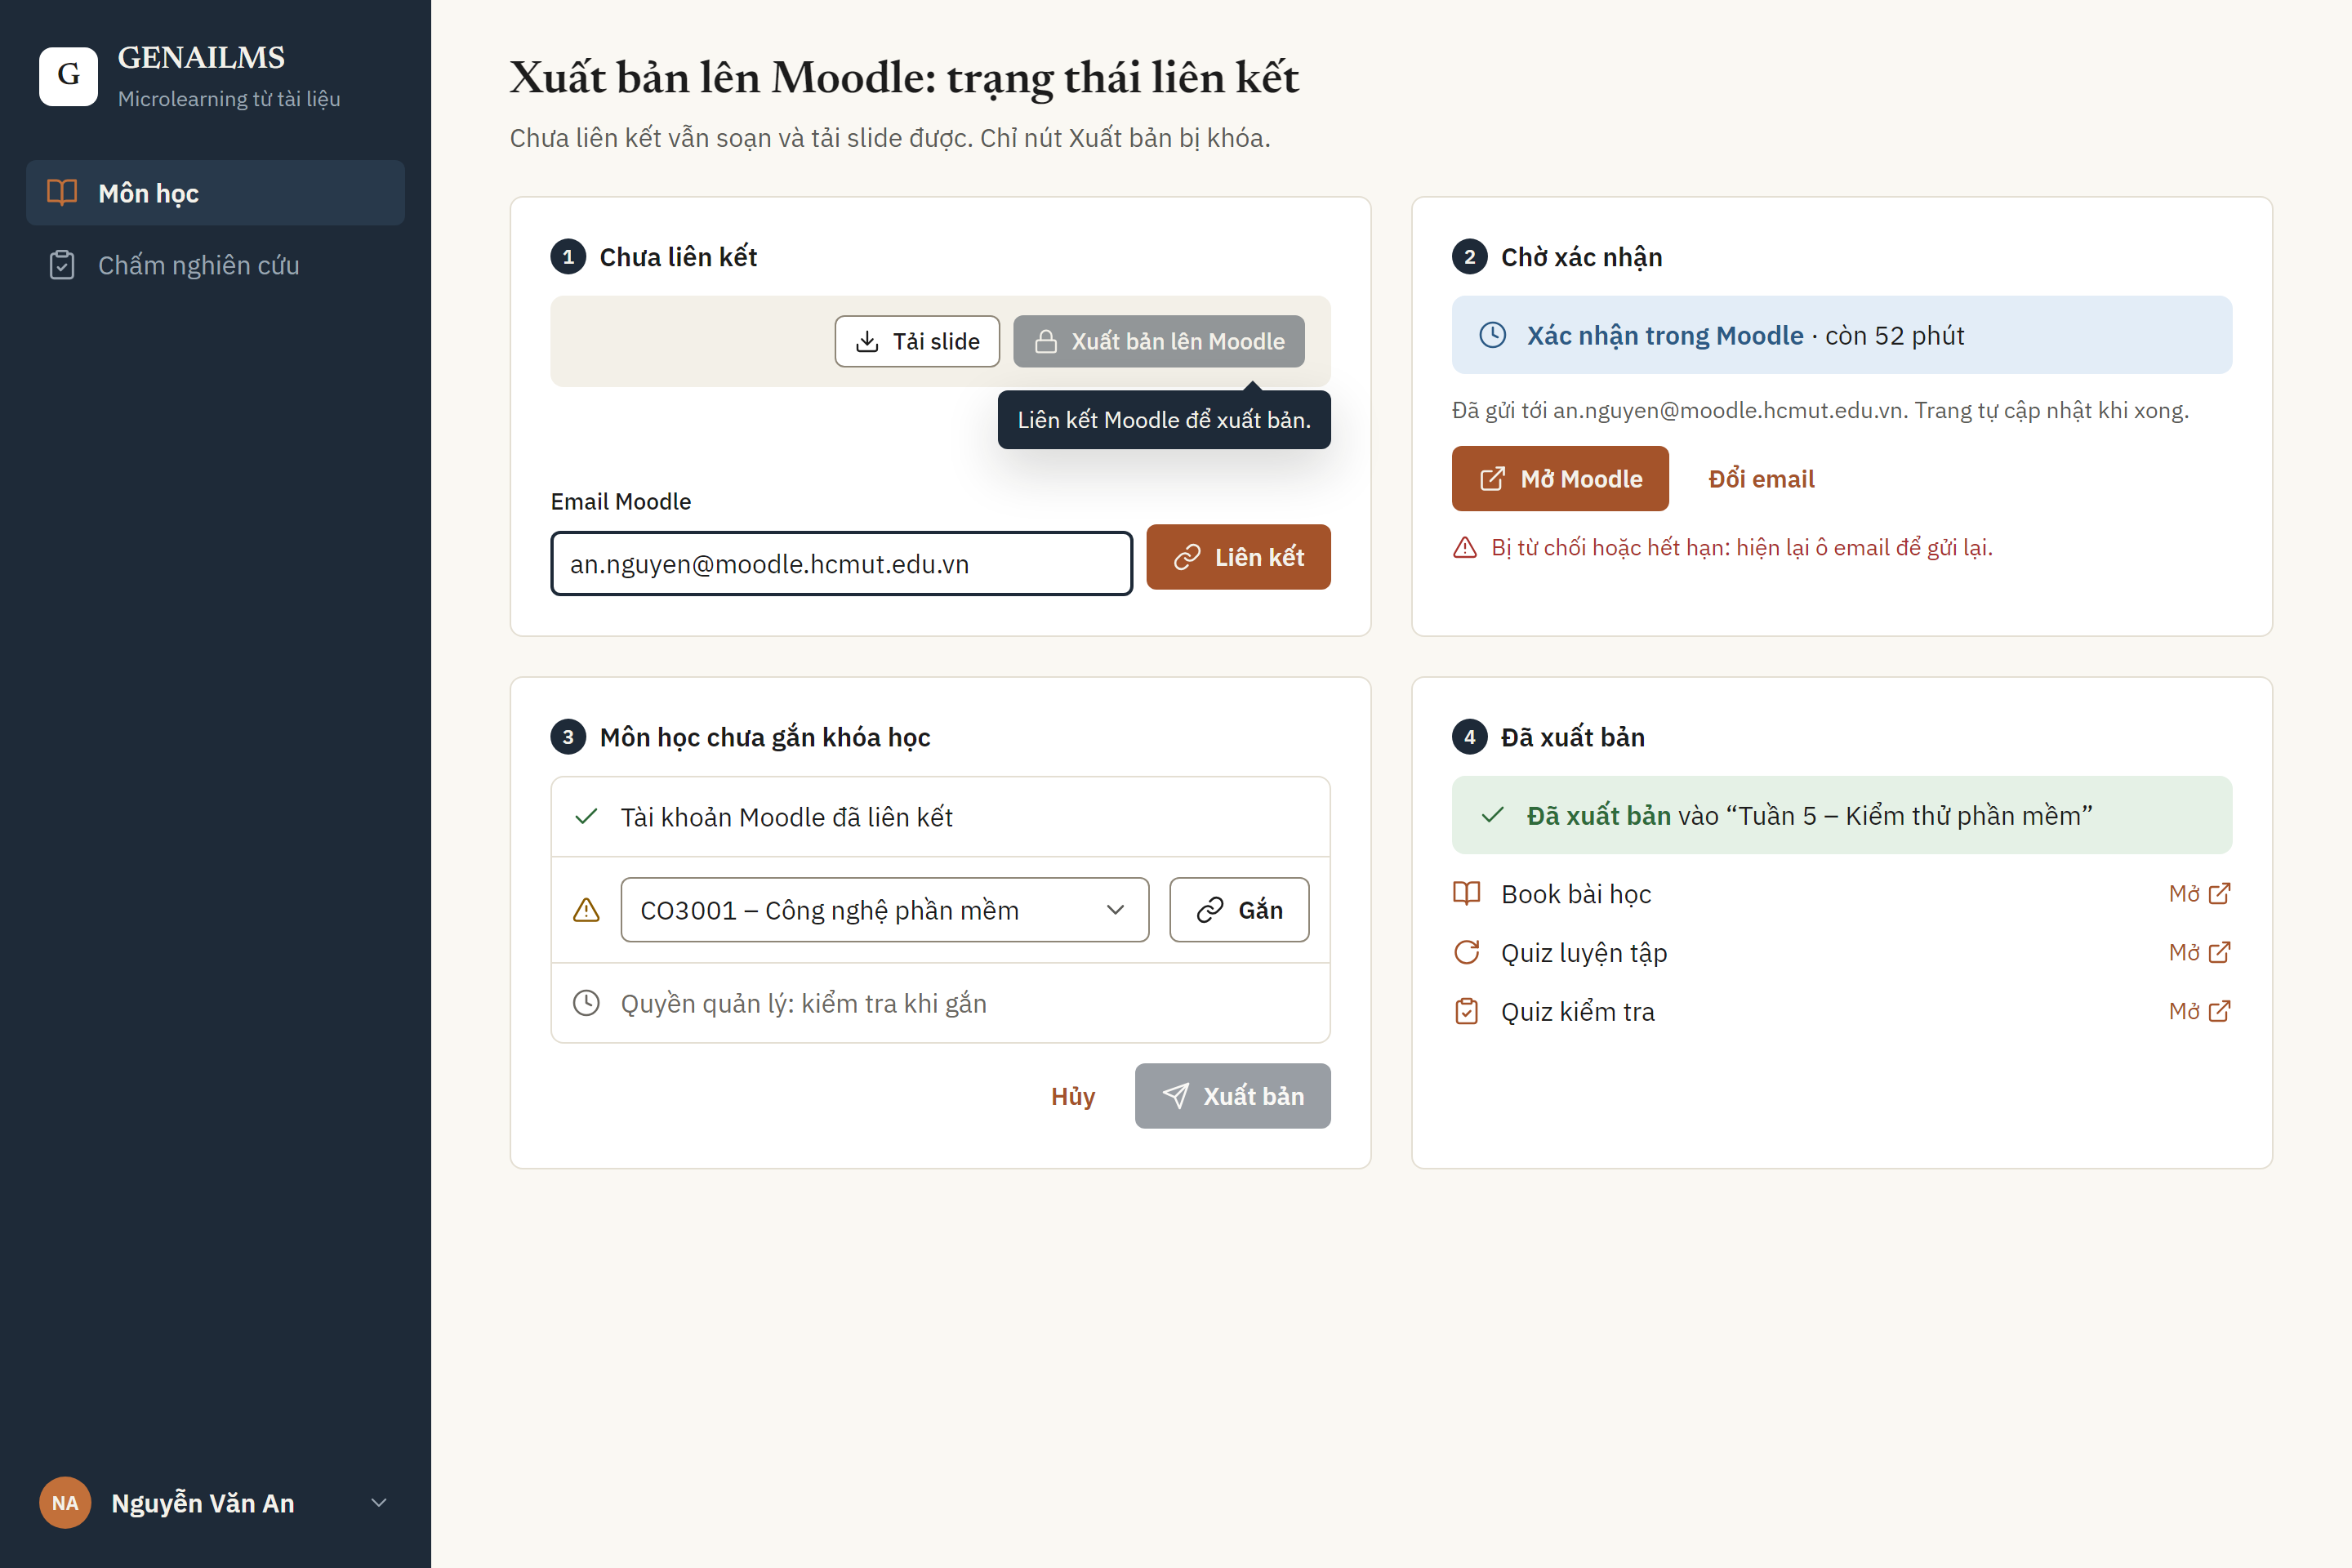
\includegraphics[width=\linewidth,height=.34\textheight,keepaspectratio,viewport={1710 1120 2810 1700},clip]{graphics/ui/09-publish-moodle-link-states.png}
\caption{Pending Moodle confirmation and next actions.}\label{fig:ui-screen-09}
\end{figure}

\needspace{.42\textheight}
The row menu in Figure~\ref{fig:ui-screen-10} groups account actions by the selected person. ``Đặt lại mật khẩu'' means ``Reset password'' and ``Vô hiệu hóa'' means ``Disable''; administrator status does not grant general access to the person's teaching content.
\begin{figure}[H]\centering
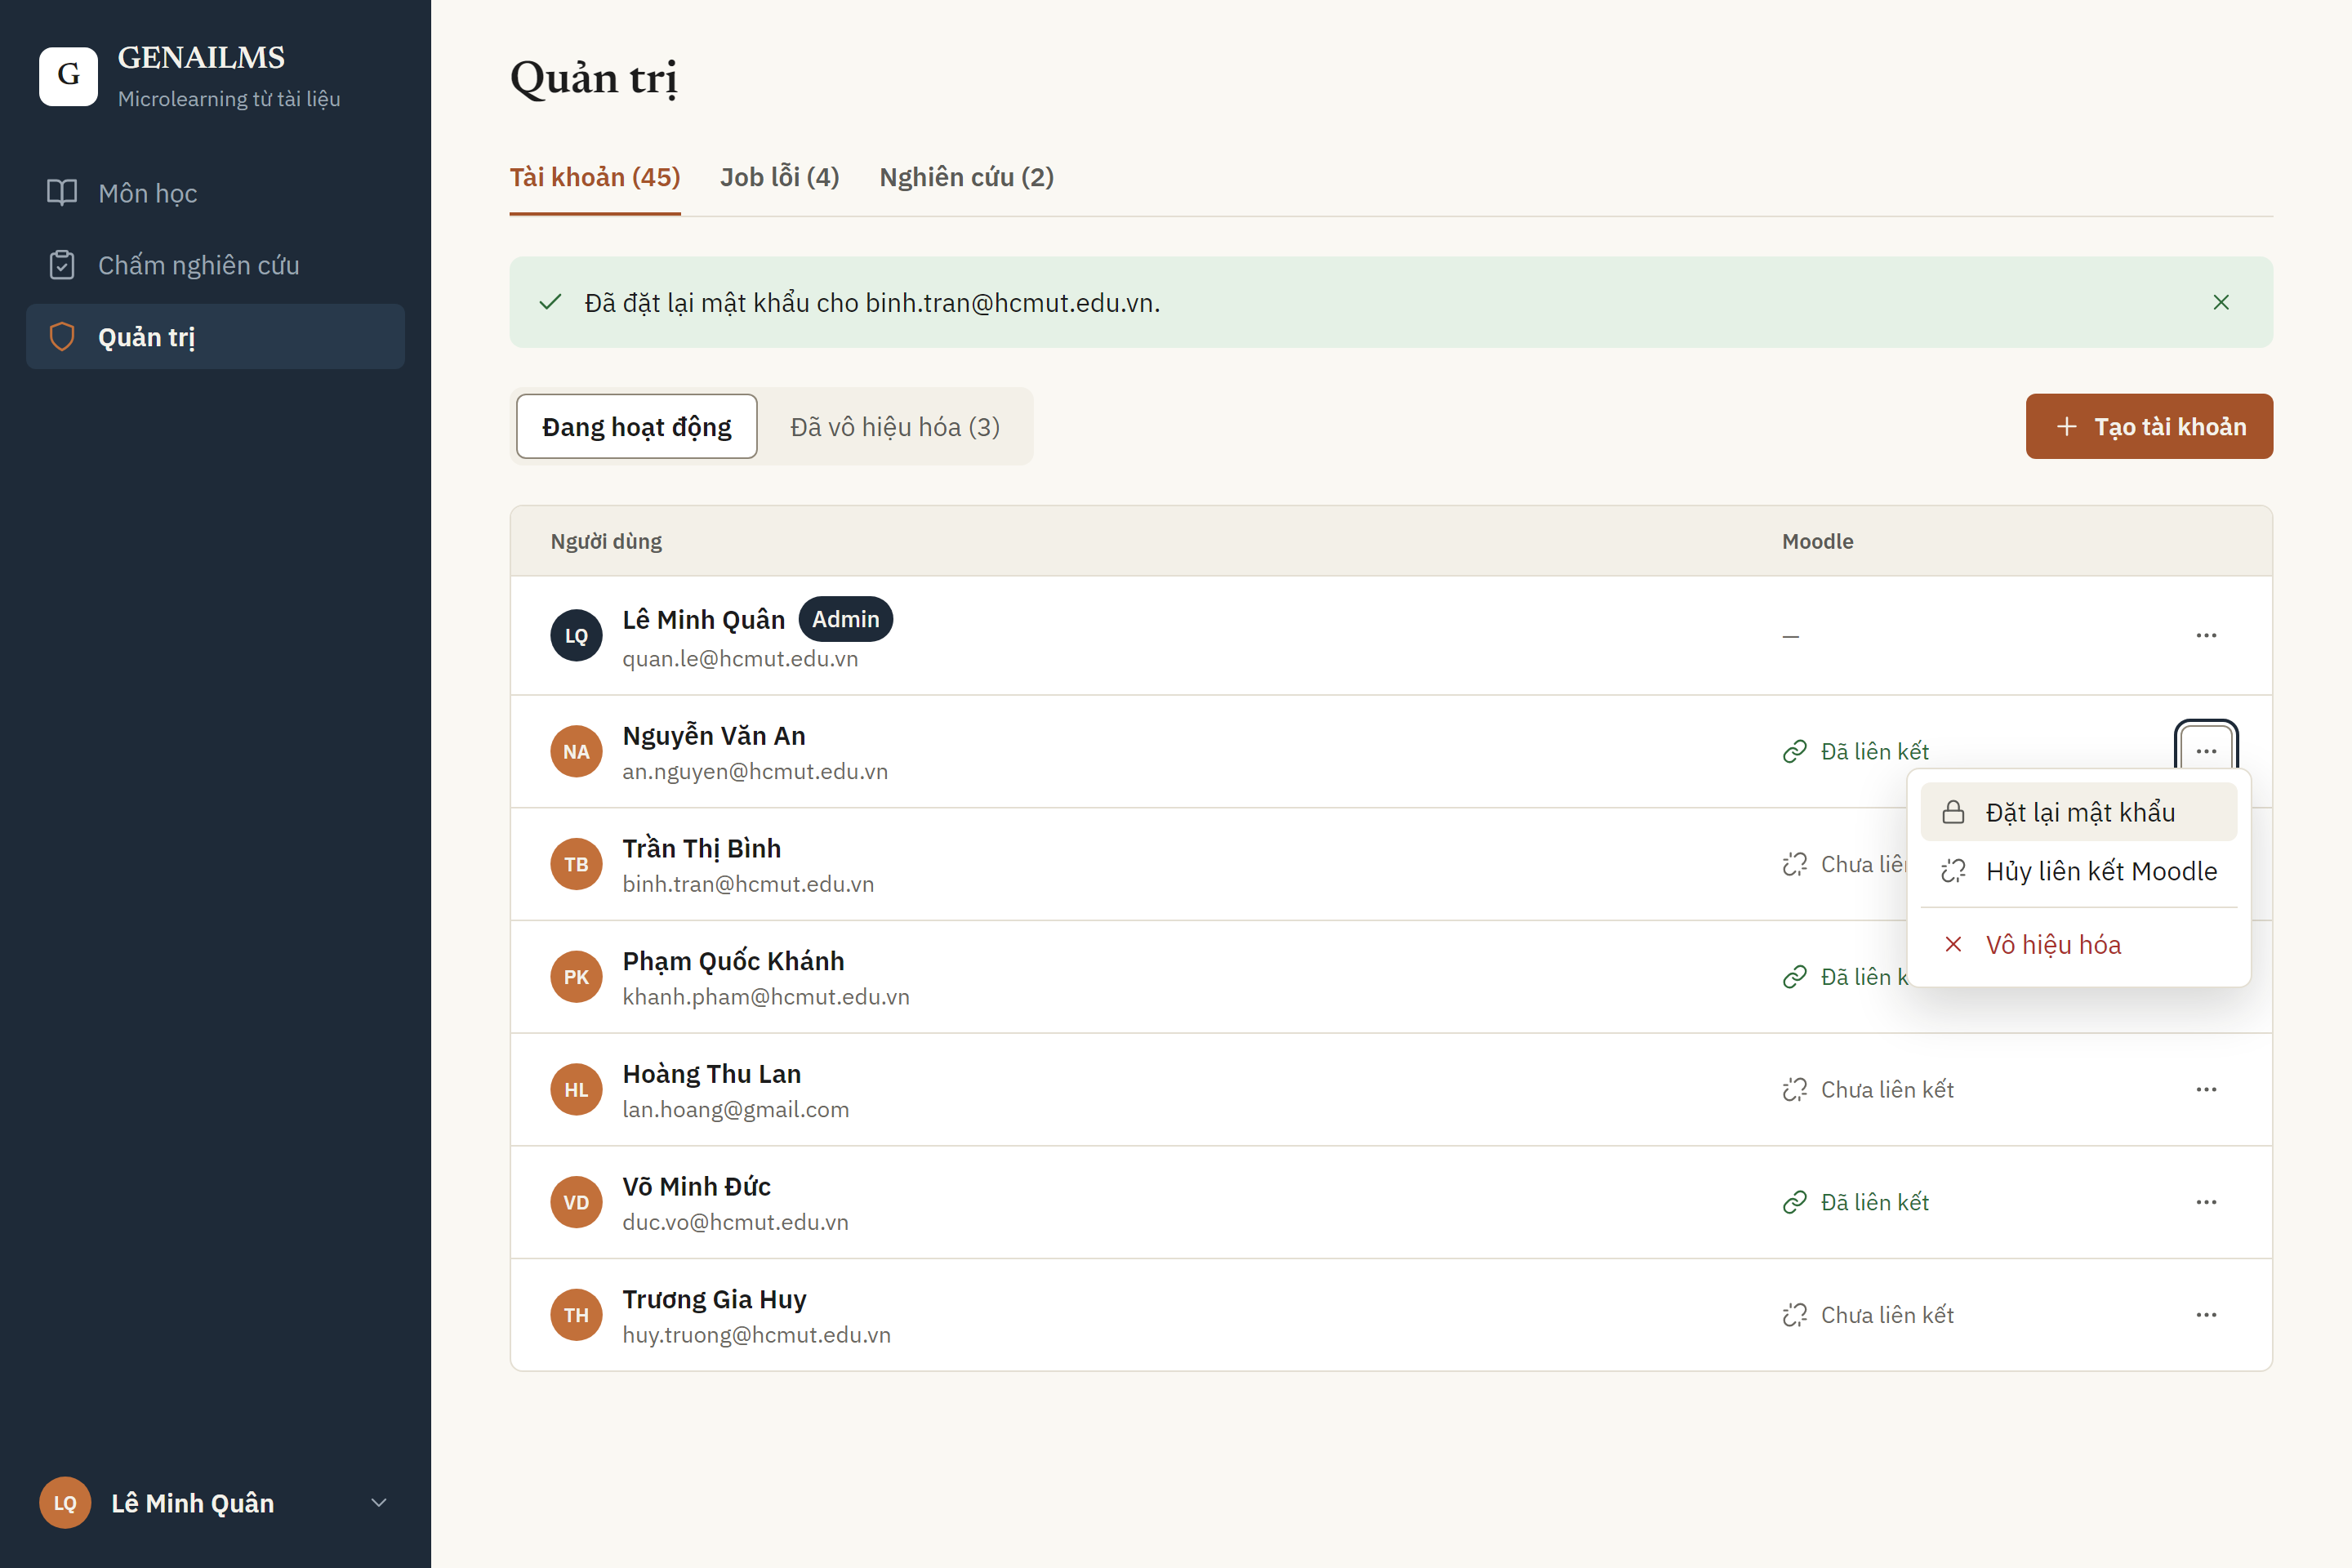
\includegraphics[width=\linewidth,height=.34\textheight,keepaspectratio,viewport={1900 650 2820 1450},clip]{graphics/ui/10-admin-accounts.png}
\caption{Contextual account-administration actions.}\label{fig:ui-screen-10}
\end{figure}

\needspace{.42\textheight}
Figure~\ref{fig:ui-screen-11} exposes failure detail and the permitted retry action. ``Thử lại'' means ``Retry''; the interface distinguishes an author's own job from the administrator's operational recovery scope.
\begin{figure}[H]\centering
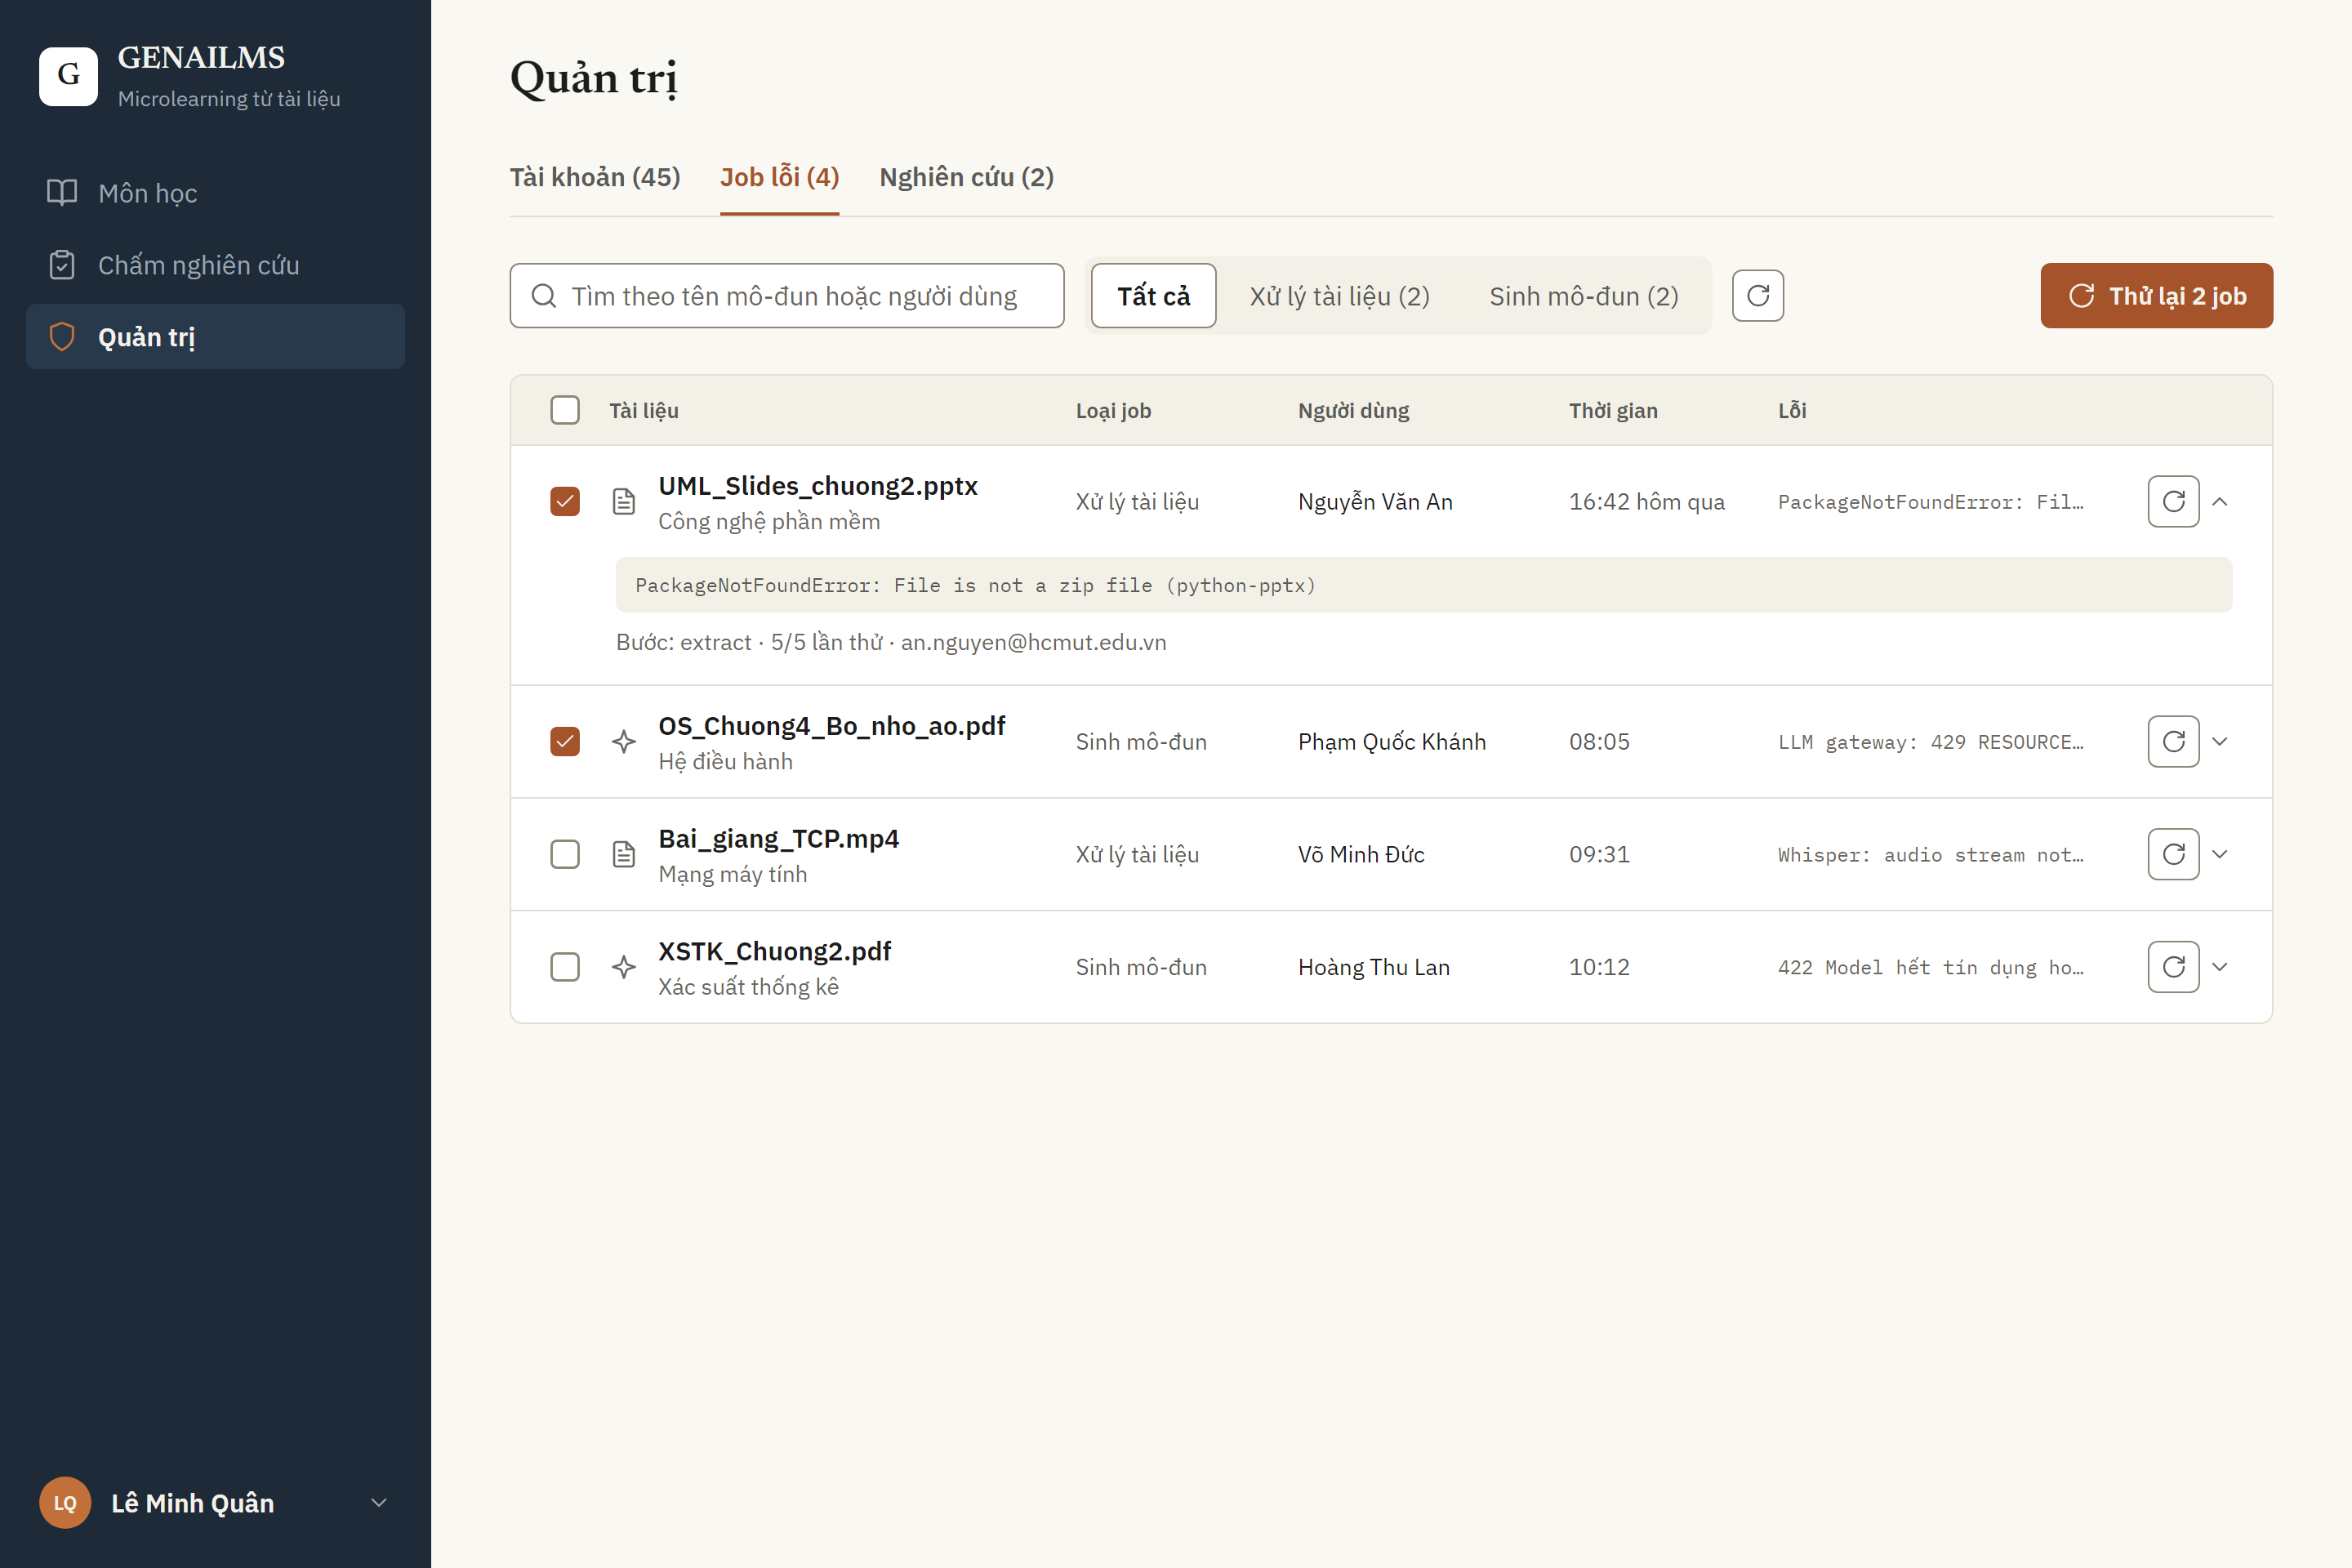
\includegraphics[width=\linewidth,height=.34\textheight,keepaspectratio,viewport={1200 850 2820 1550},clip]{graphics/ui/11-admin-failed-jobs.png}
\caption{Failed-job inspection and recovery.}\label{fig:ui-screen-11}
\end{figure}

\needspace{.42\textheight}
Figure~\ref{fig:ui-screen-12} groups study identity, snapshot preparation and rater invitations in an administrative workspace. ``Nghiên cứu'' means ``Study''; anonymous packet preparation precedes activation for raters.
\begin{figure}[H]\centering
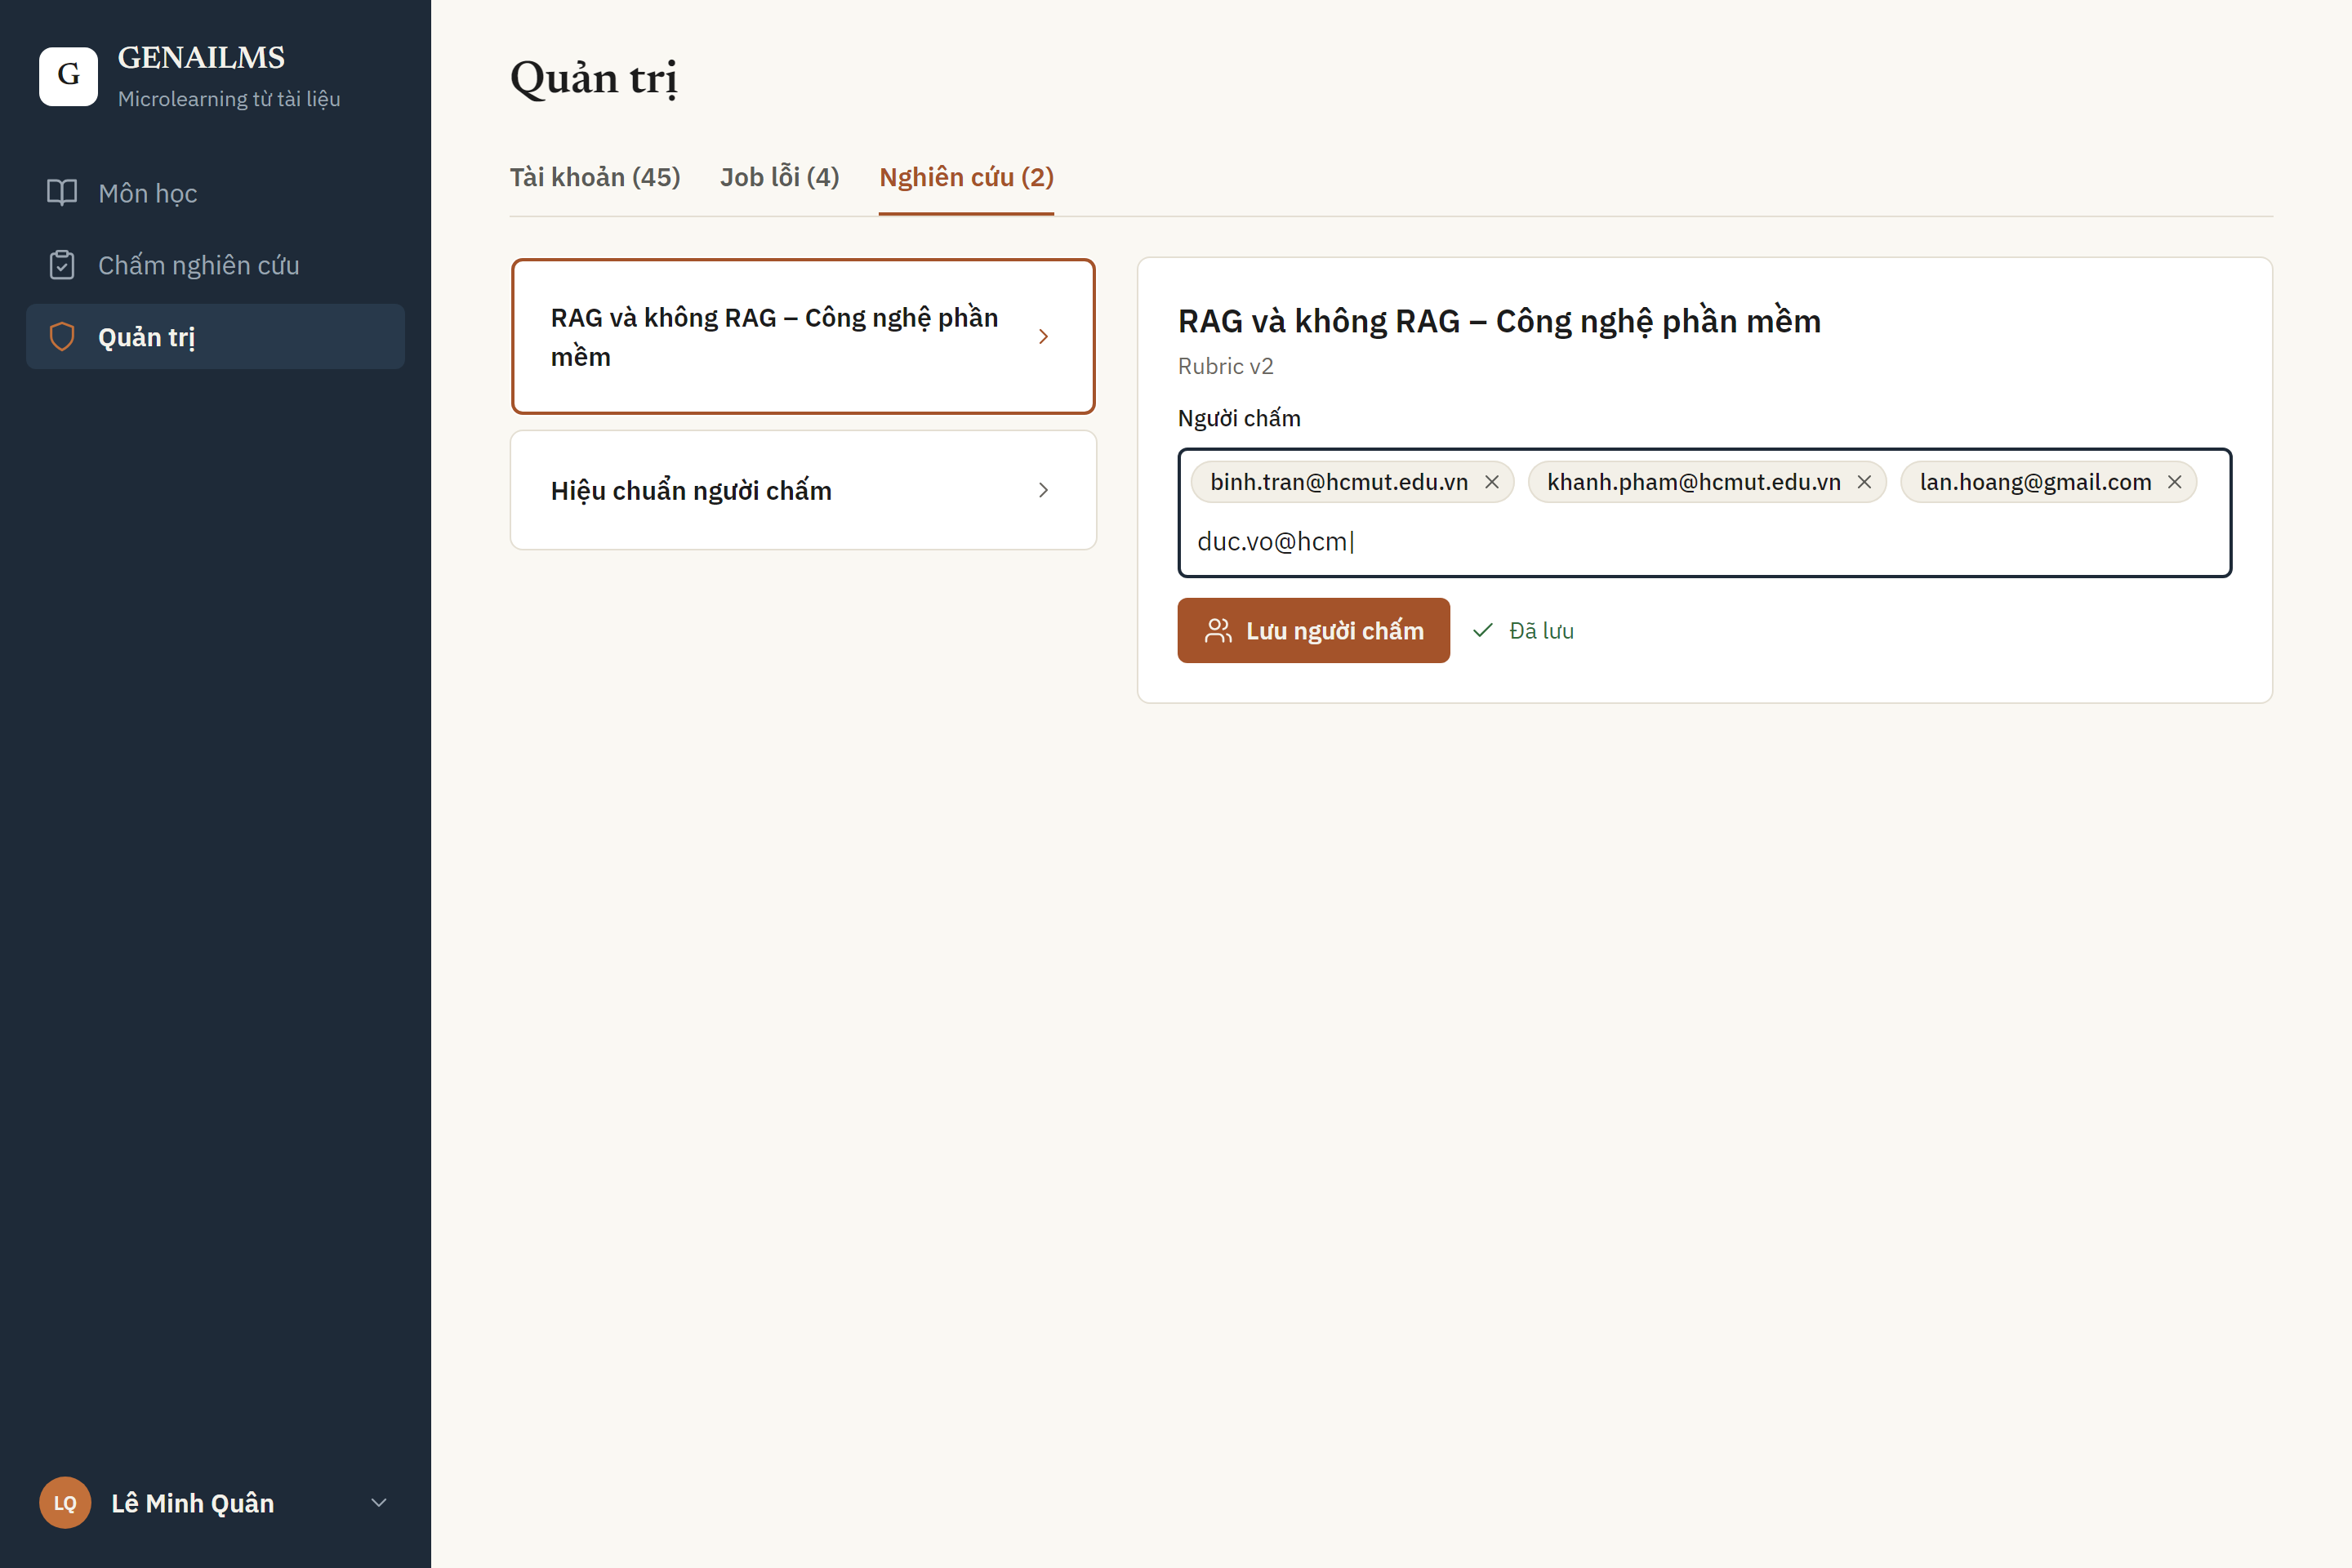
\includegraphics[width=\linewidth,height=.34\textheight,keepaspectratio,viewport={1370 1030 2810 1630},clip]{graphics/ui/12-admin-studies.png}
\caption{Study preparation and invitations.}\label{fig:ui-screen-12}
\end{figure}

\needspace{.42\textheight}
Figure~\ref{fig:ui-screen-13} enlarges the scoring controls and the reason field in the blinded-rating screen. ``Nhận xét'' means ``Comment''; the 1--5 controls and written reasons are recorded per criterion while the packet order remains stable for the rater.
\begin{figure}[H]\centering
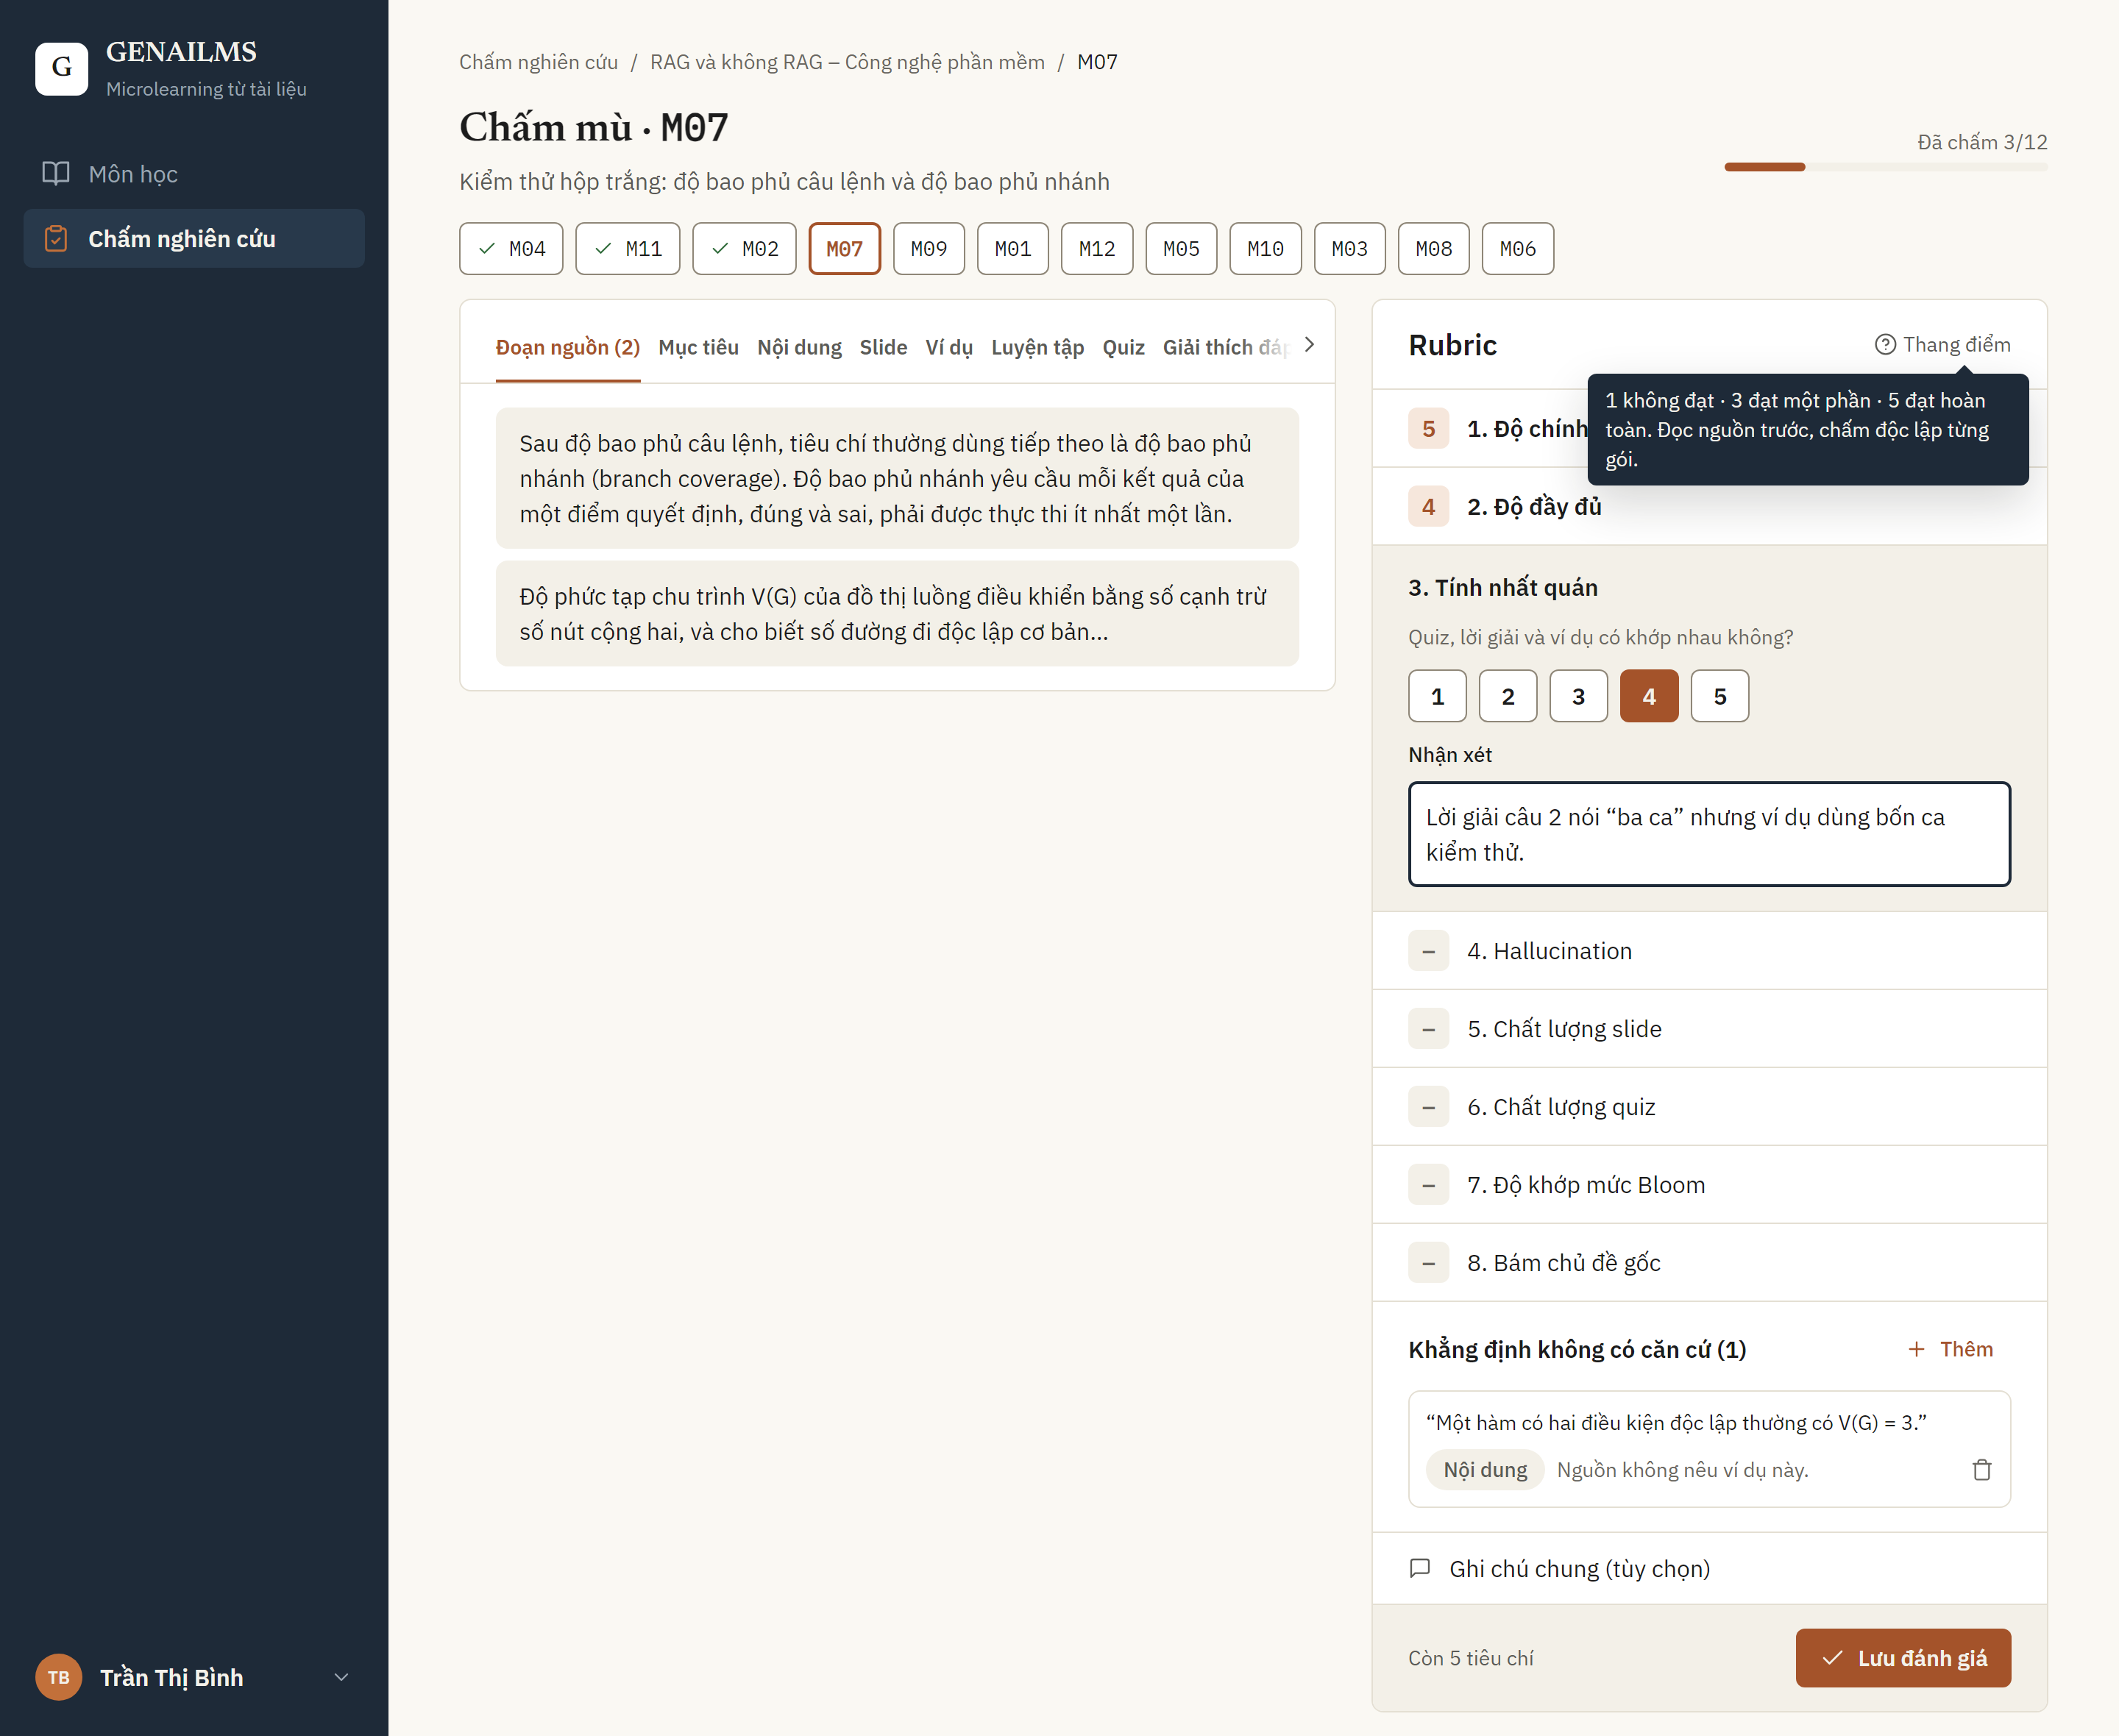
\includegraphics[width=\linewidth,height=.34\textheight,keepaspectratio,viewport={1850 1100 2800 1580},clip]{graphics/ui/13-rater-blind-rating.png}
\caption{Focused rubric and criterion-level reasoning.}\label{fig:ui-screen-13}
\end{figure}

\needspace{.42\textheight}
Figure~\ref{fig:ui-screen-14} shows the course workspace as a single column on a mobile viewport. Upload, status and generation actions retain text labels; secondary information collapses without hiding failure recovery.
\begin{figure}[H]\centering
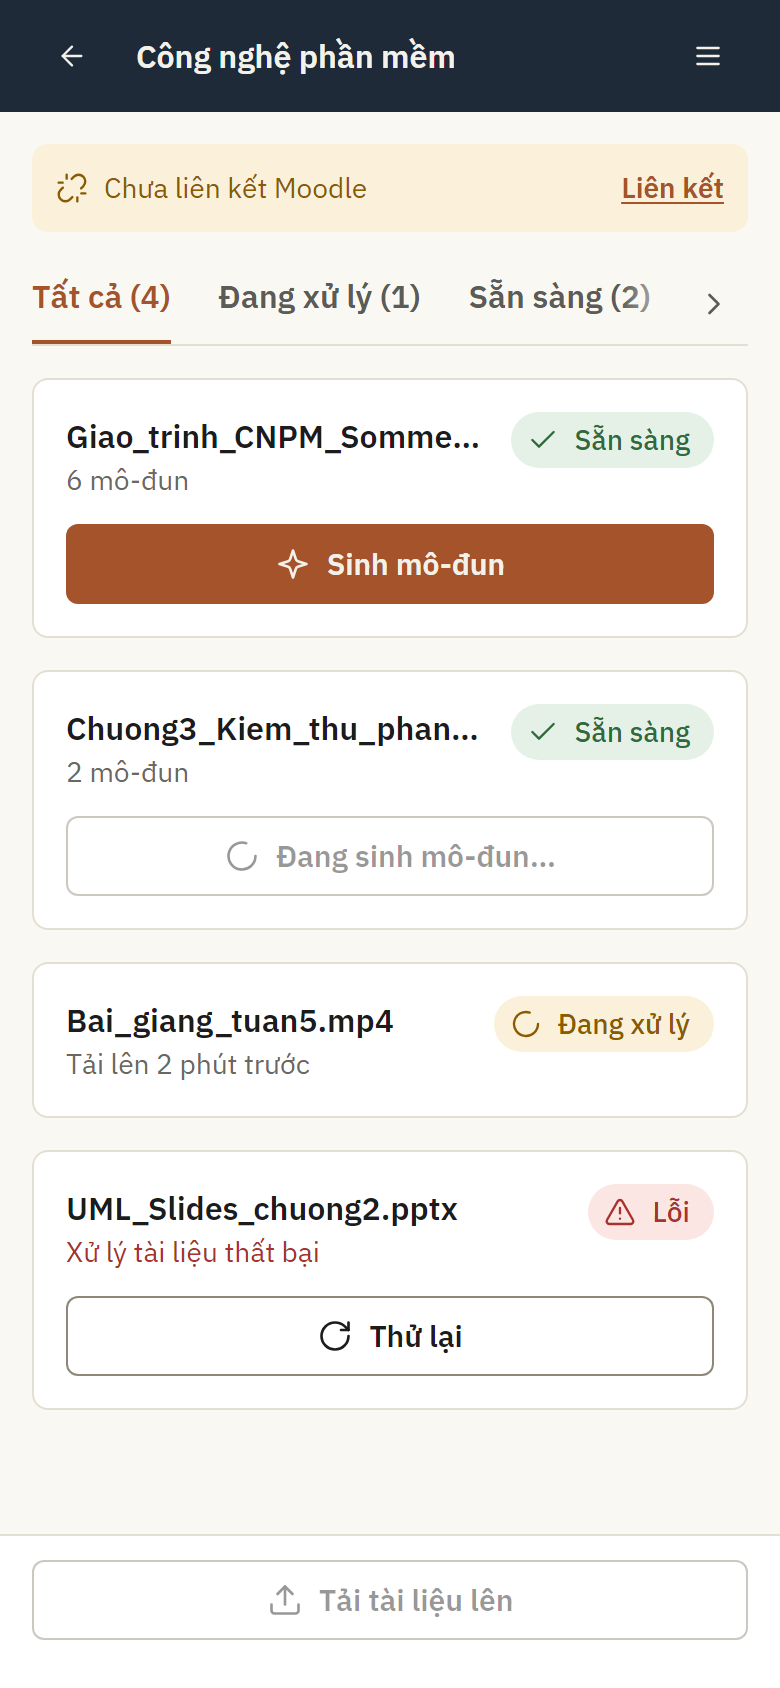
\includegraphics[width=.65\linewidth,height=.60\textheight,keepaspectratio]{graphics/ui/14-mobile-course-detail.png}
\caption{Mobile authoring workspace.}\label{fig:ui-screen-14}
\end{figure}

\needspace{.42\textheight}
Figure~\ref{fig:ui-screen-15} shows empty-course, empty-document and loading panels. ``Chưa có môn học'' means ``No courses yet'' and ``Chọn tệp'' means ``Choose file''; useful next actions appear directly in the empty state.
\begin{figure}[H]\centering
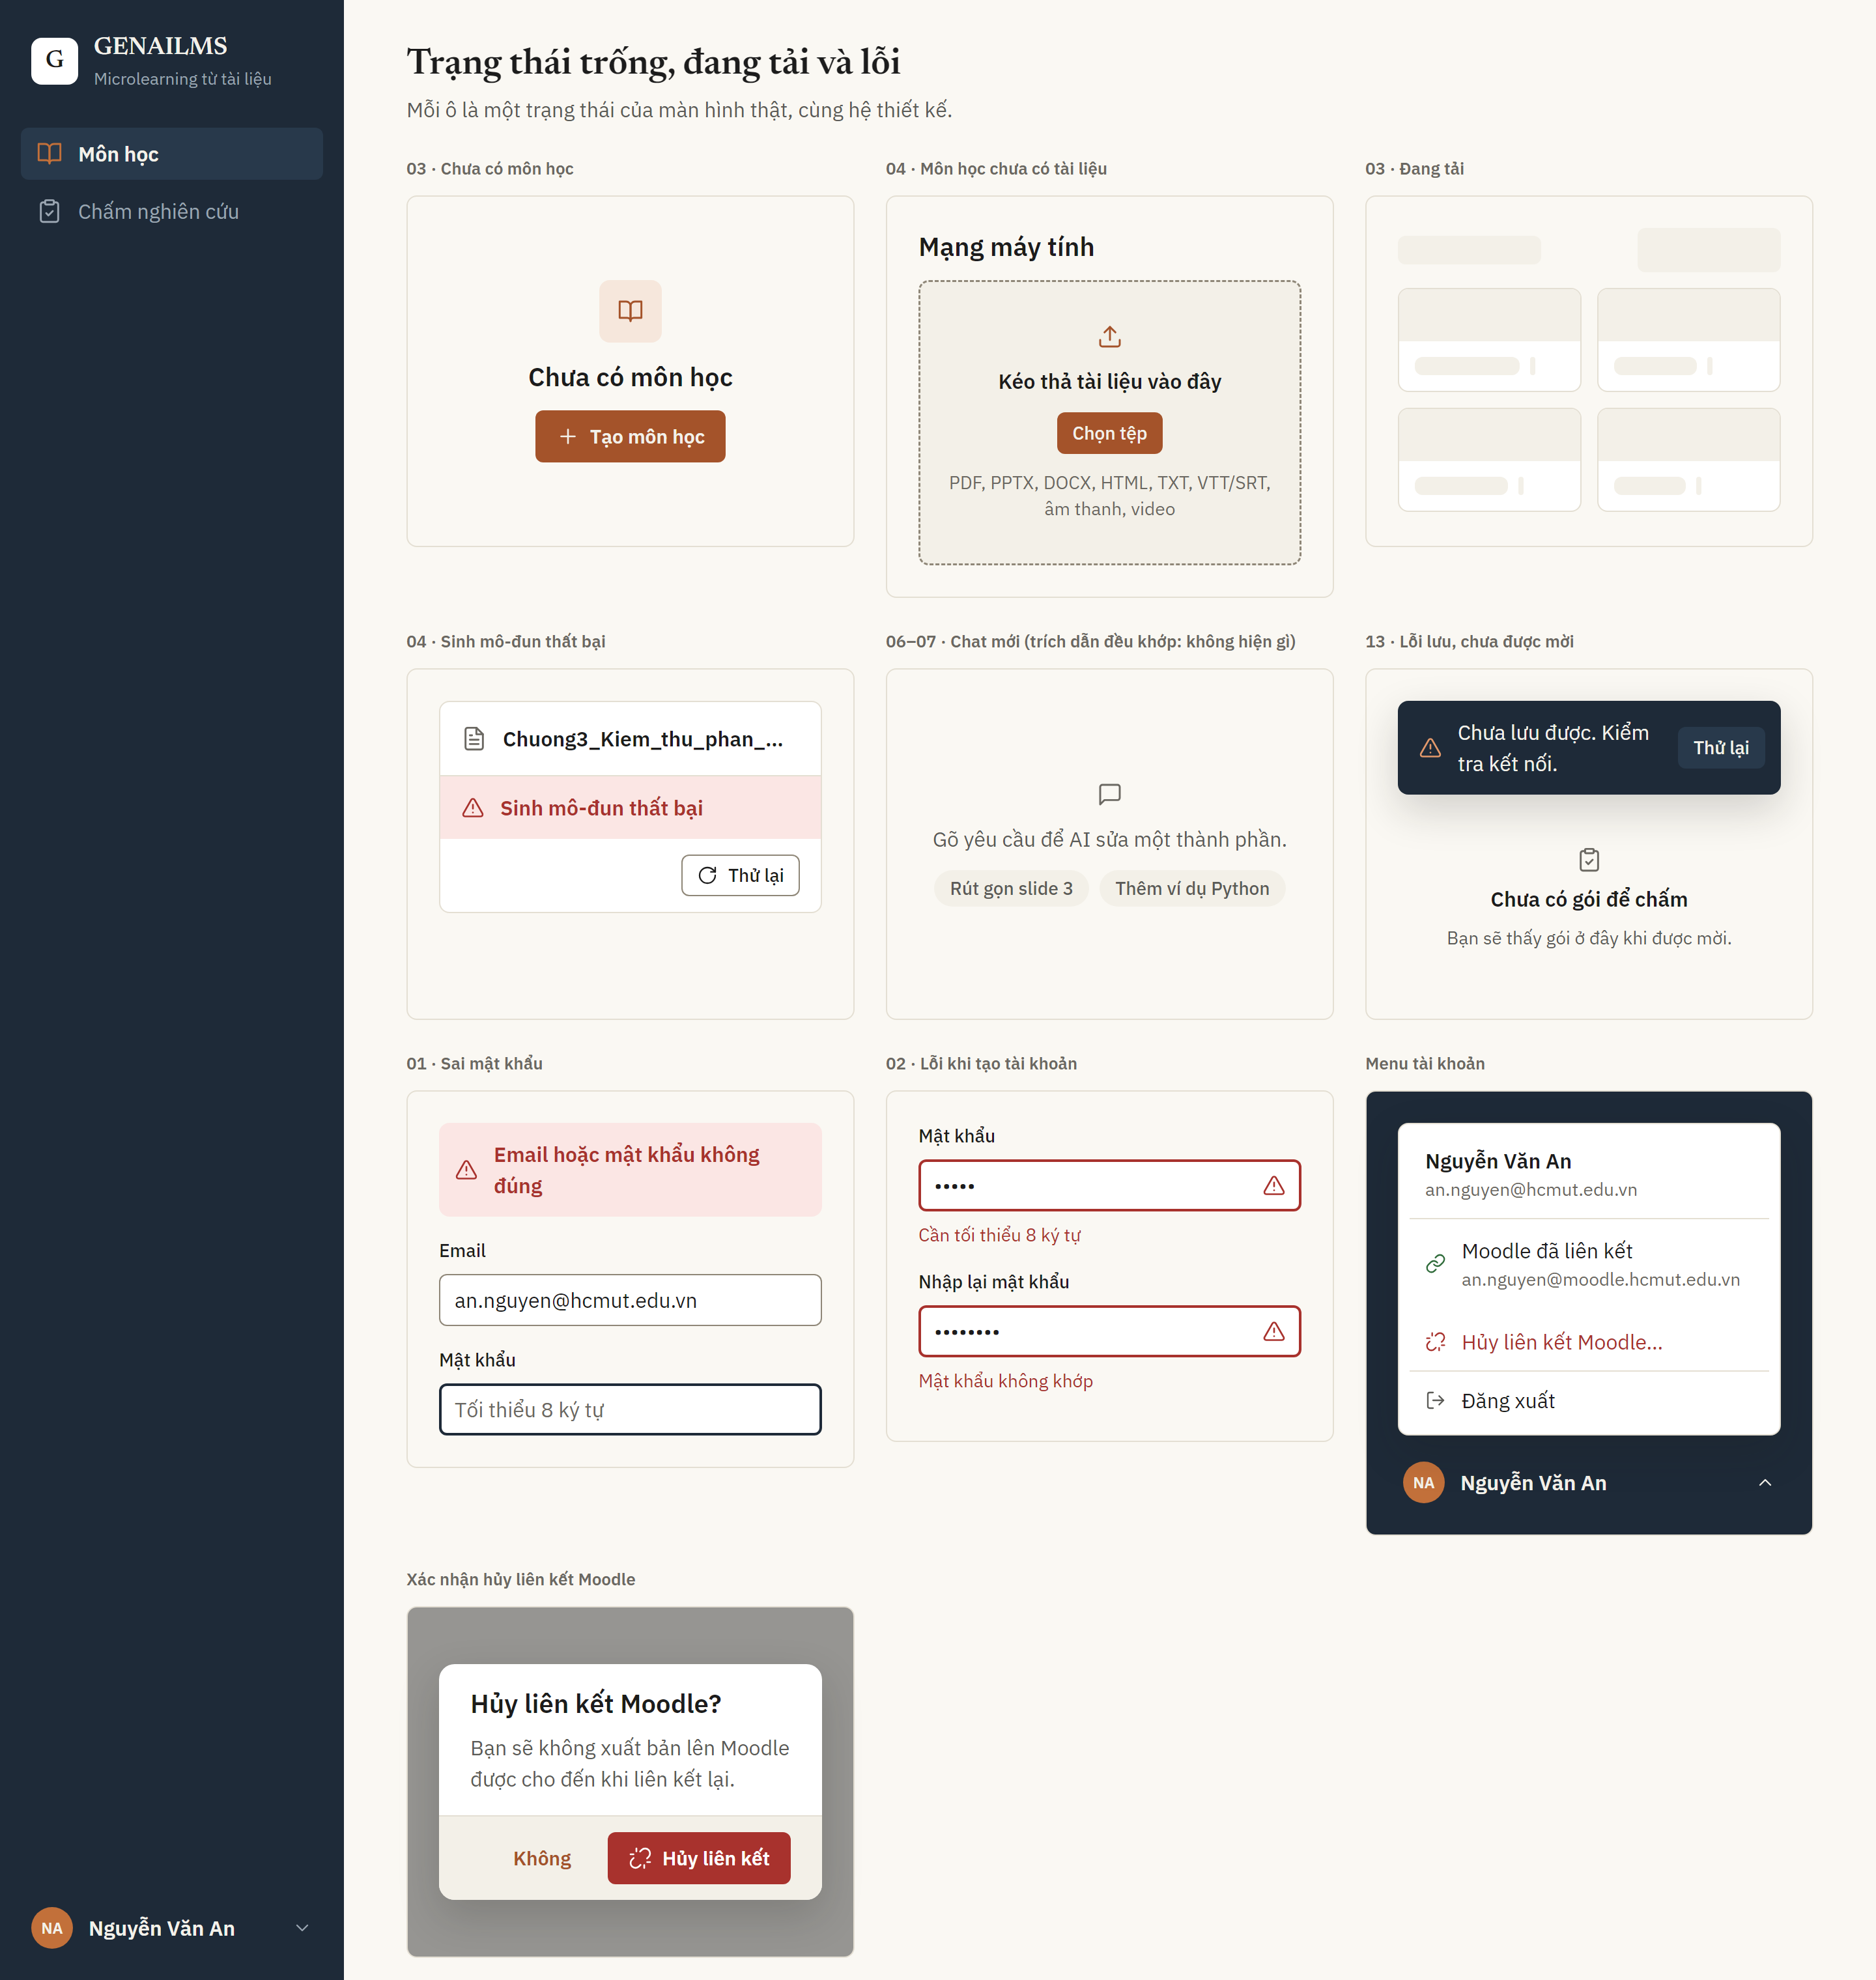
\includegraphics[width=.47\linewidth,height=.26\textheight,keepaspectratio,viewport={620 2200 1320 2750},clip]{graphics/ui/15-empty-loading-error-states.png}\hfill
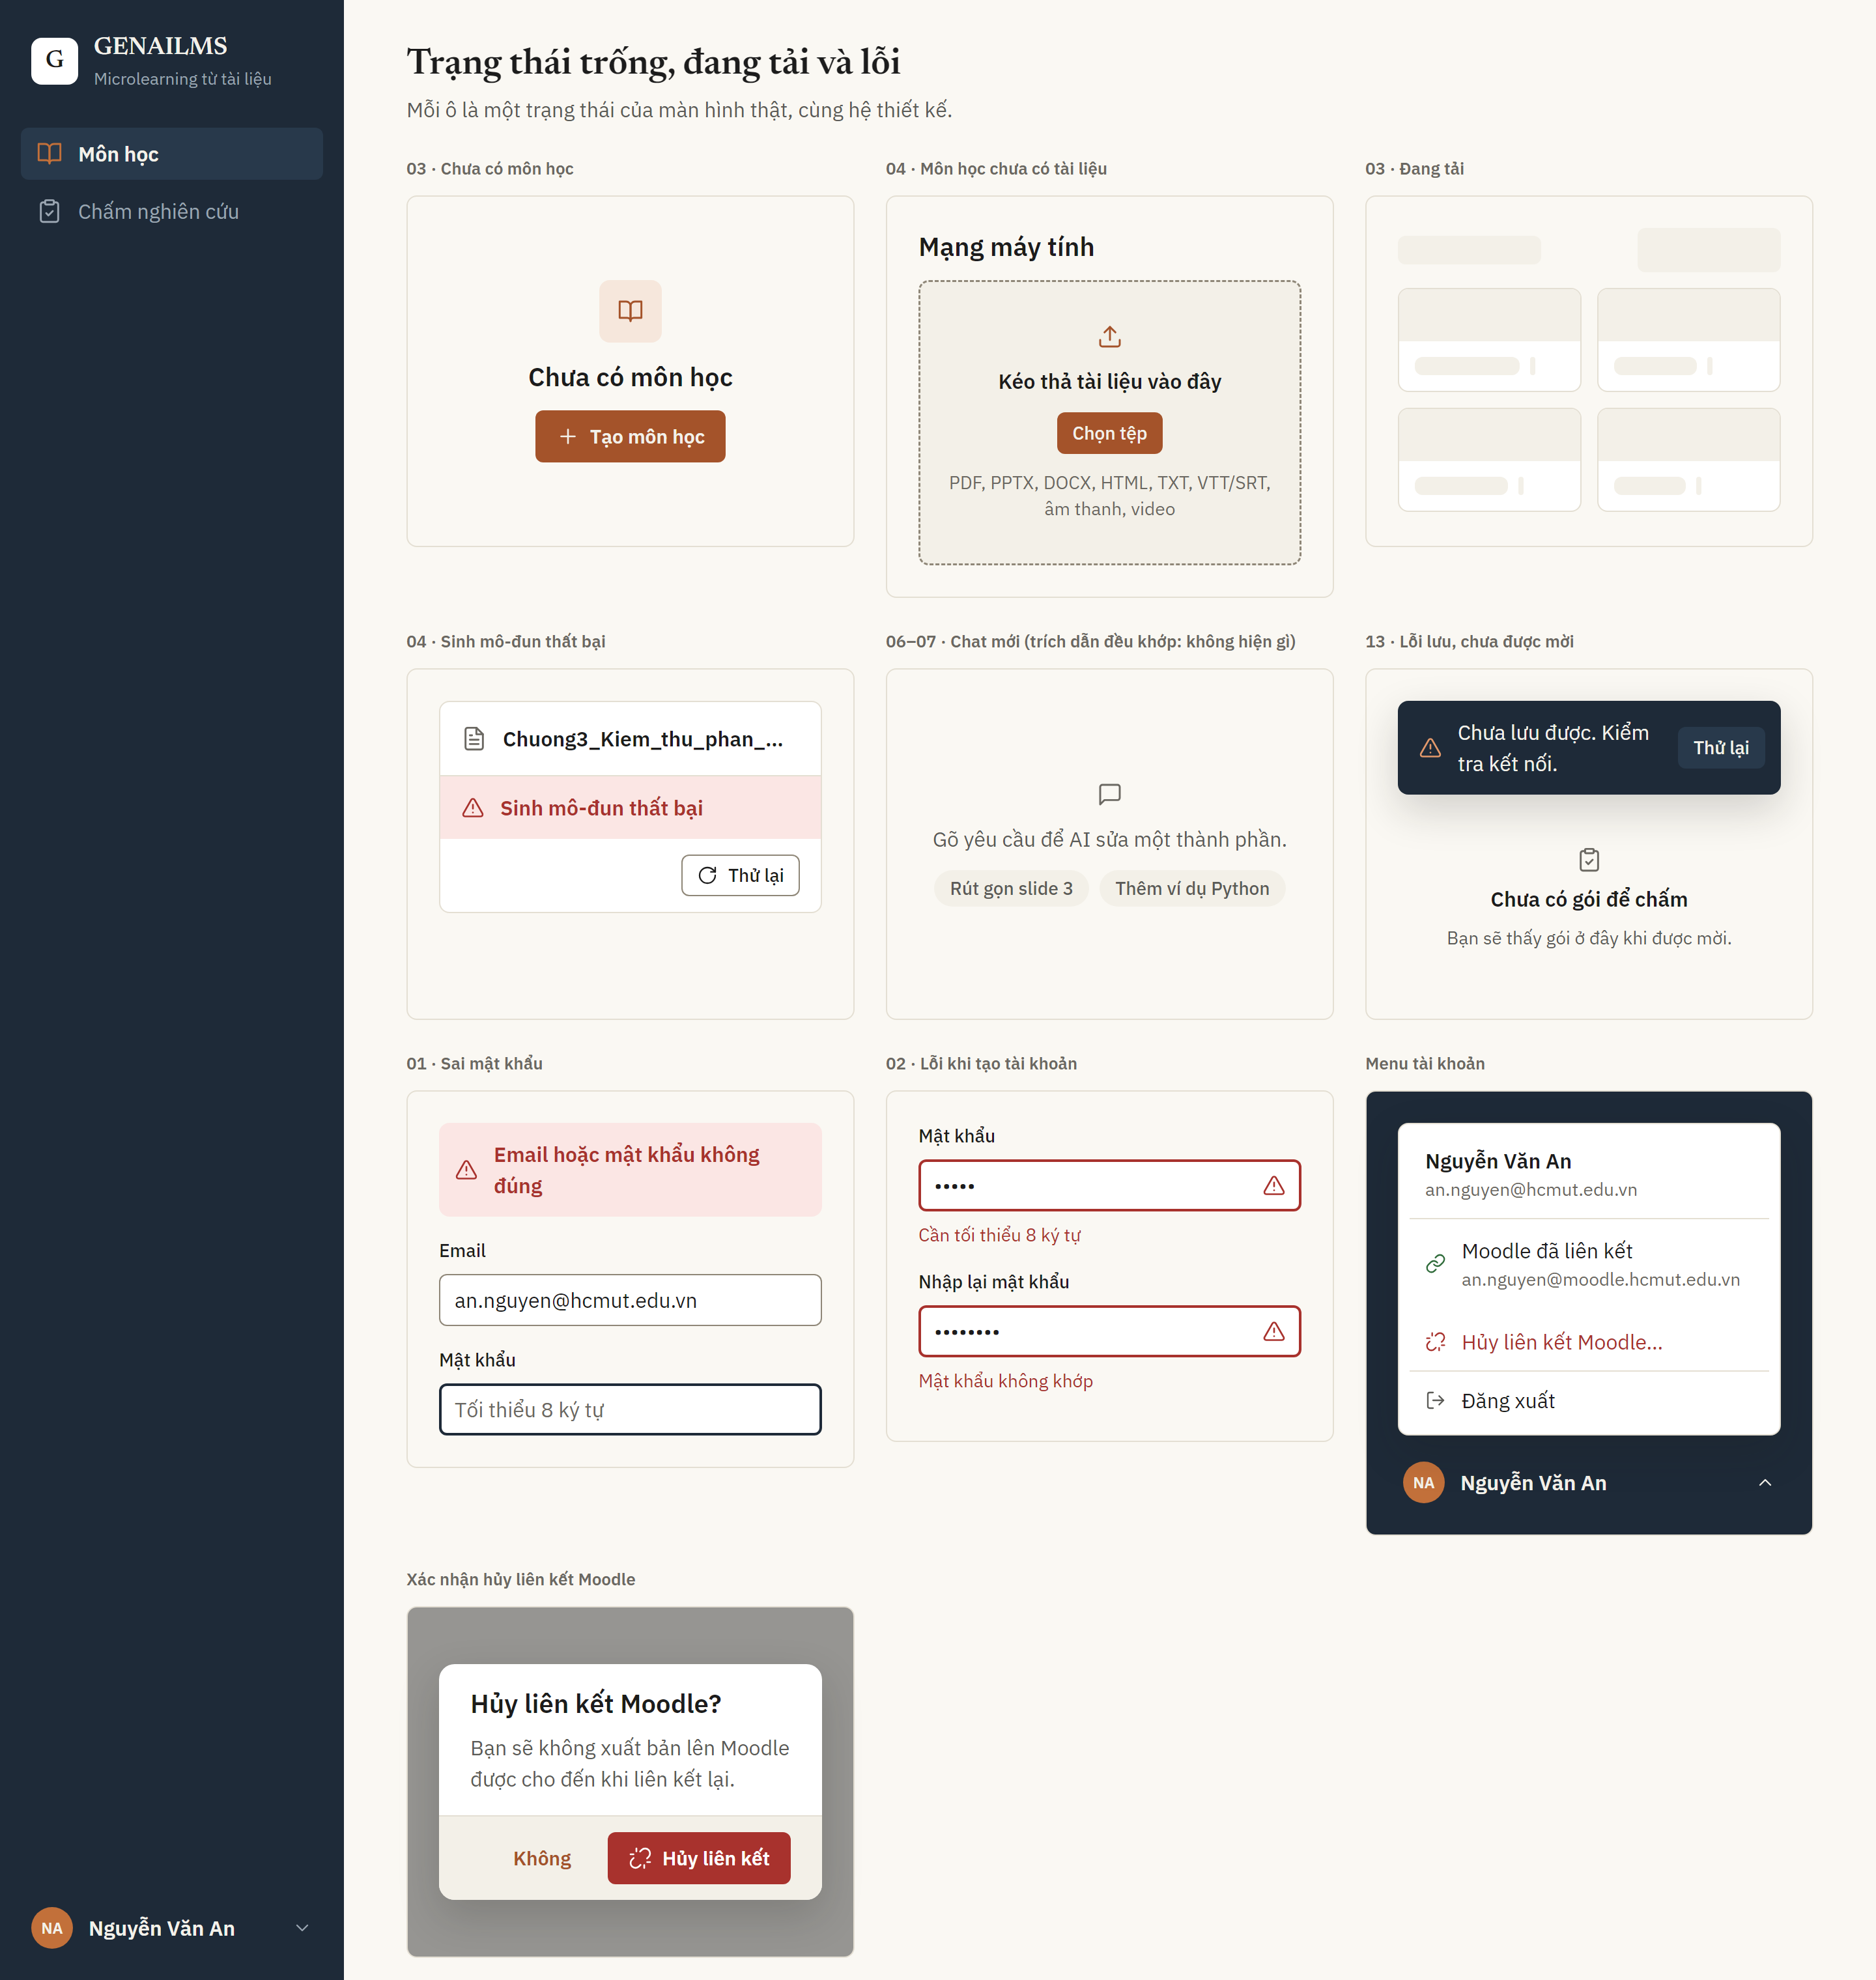
\includegraphics[width=.47\linewidth,height=.26\textheight,keepaspectratio,viewport={1360 2110 2050 2750},clip]{graphics/ui/15-empty-loading-error-states.png}\par\smallskip
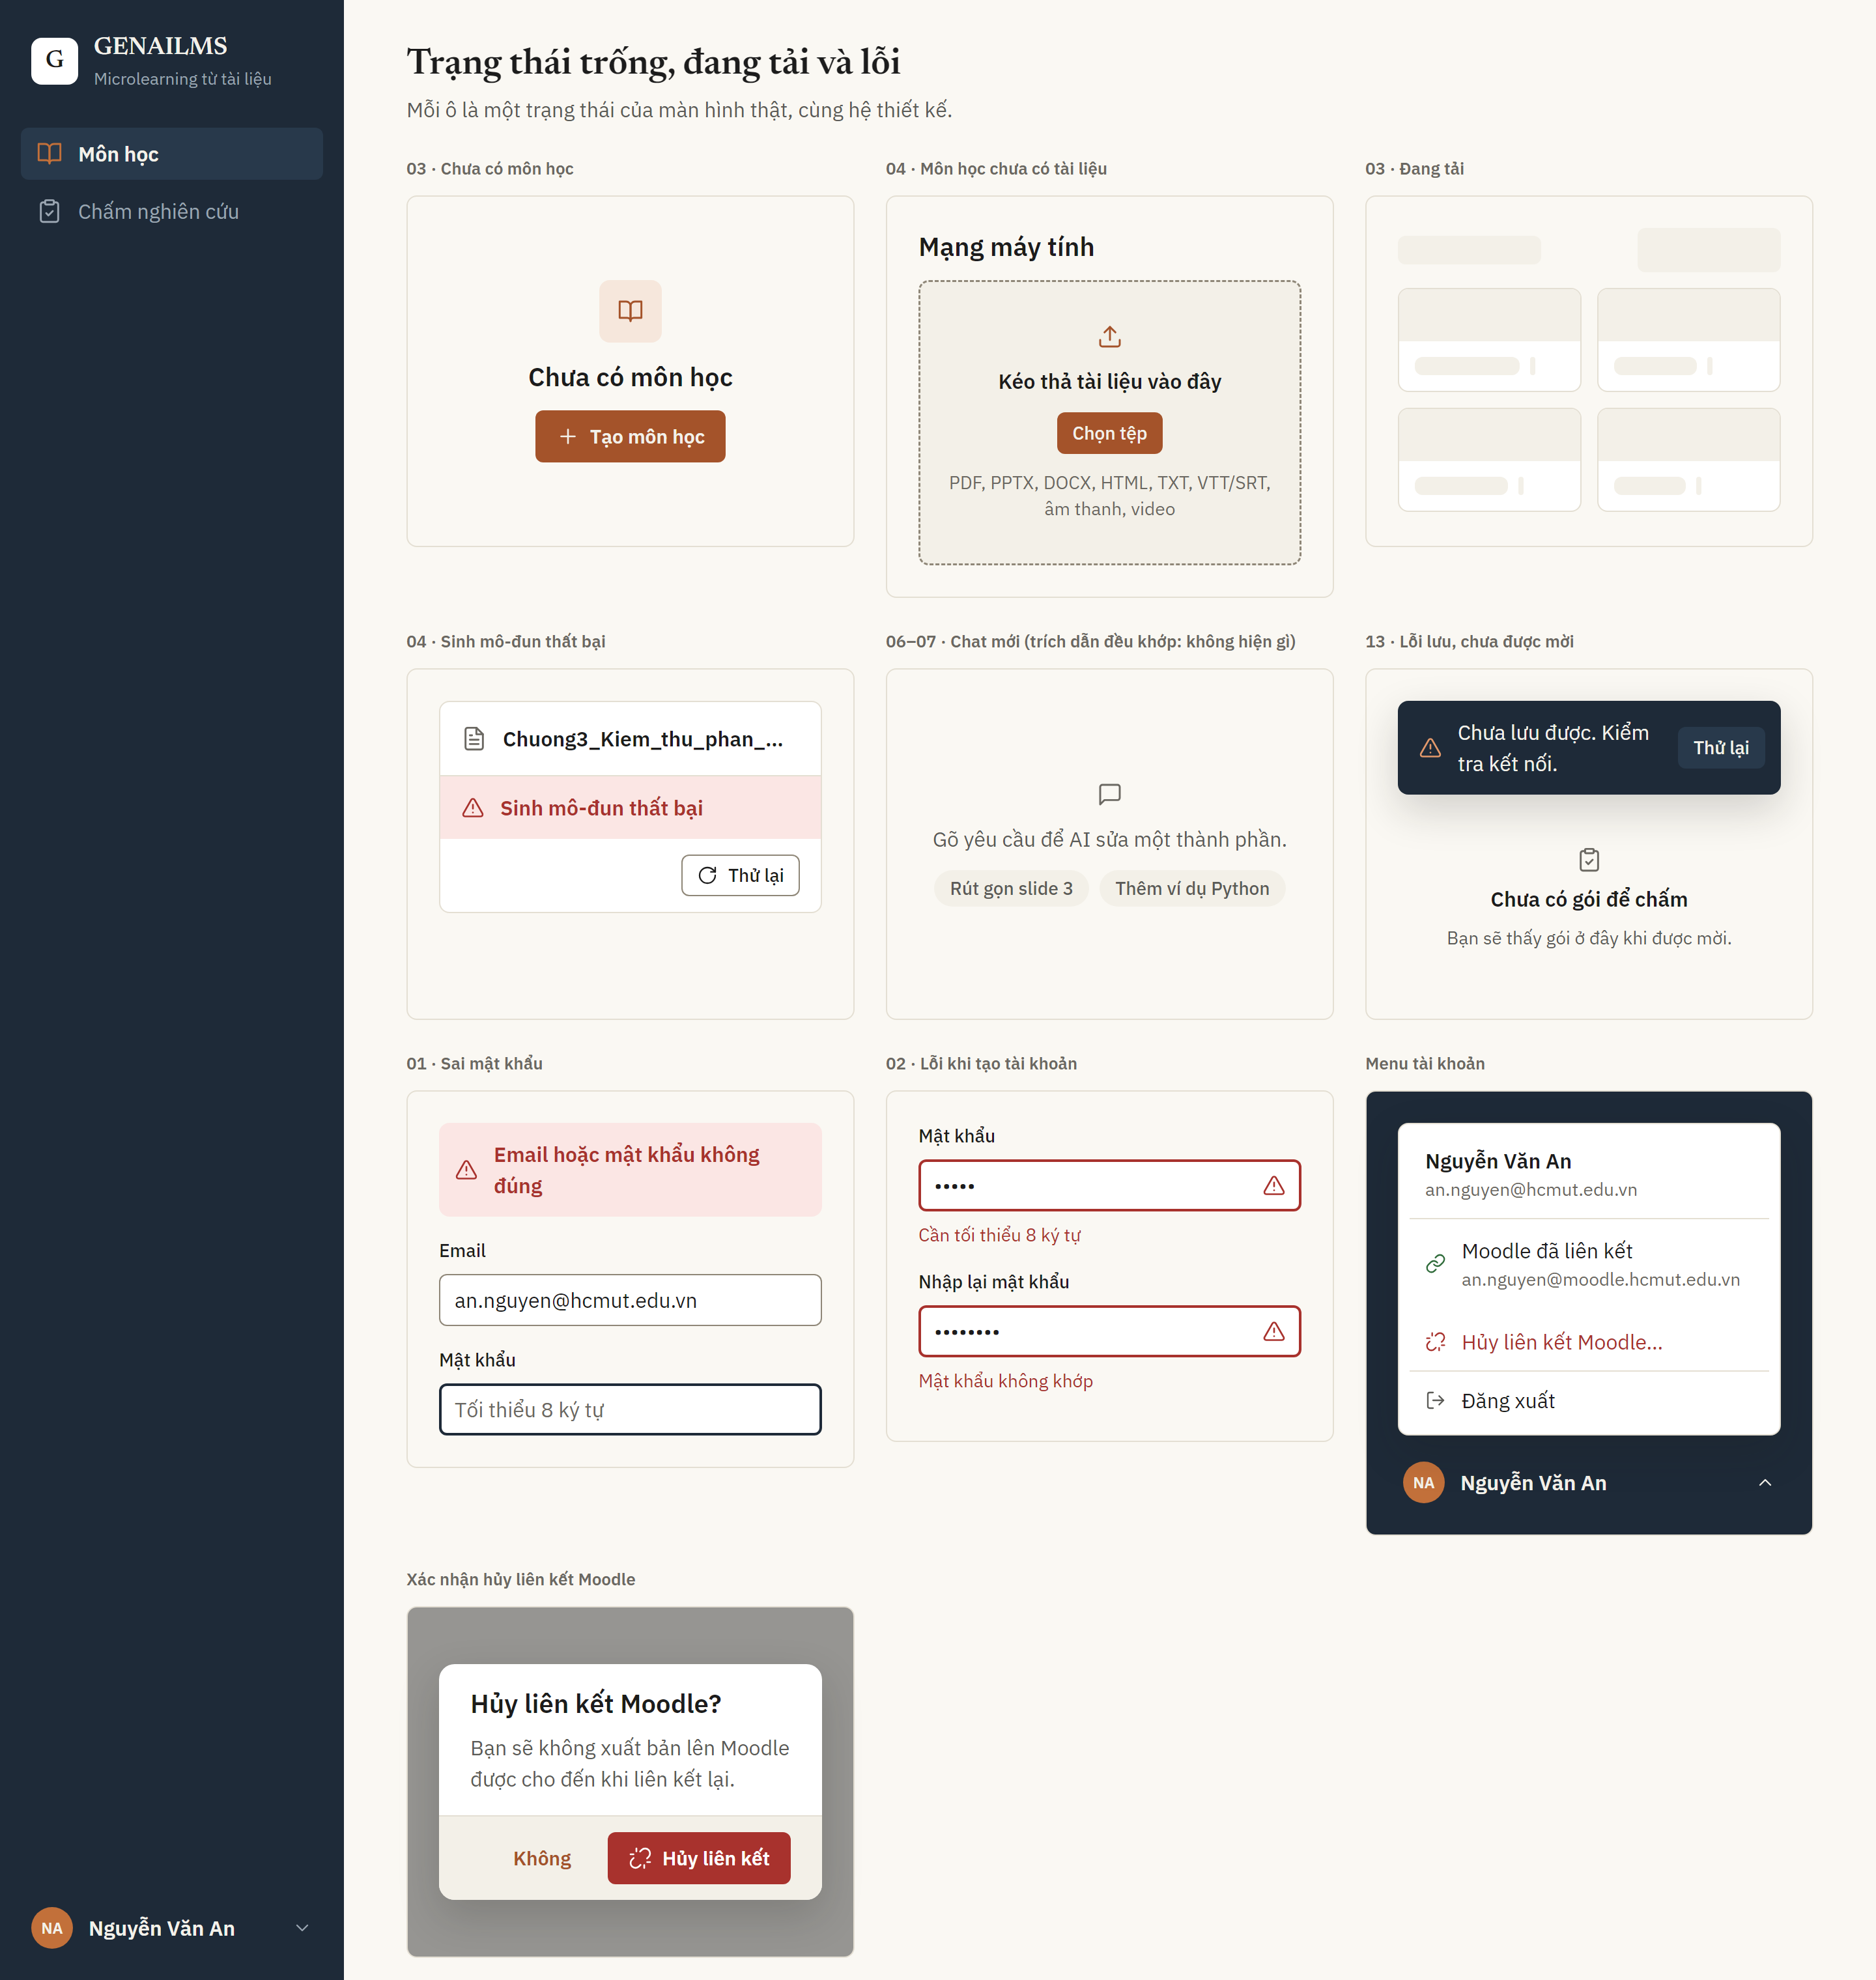
\includegraphics[width=.47\linewidth,height=.26\textheight,keepaspectratio,viewport={2100 2200 2800 2750},clip]{graphics/ui/15-empty-loading-error-states.png}\hfill
\caption{Empty and loading states.}\label{fig:ui-screen-15}
\end{figure}

\needspace{.42\textheight}
Figure~\ref{fig:ui-screen-15-recovery} groups generation failure, an empty editing conversation and a failed rating save. ``Chưa lưu được'' means ``Could not save''; the interface preserves entered work and offers retry.
\begin{figure}[H]\centering
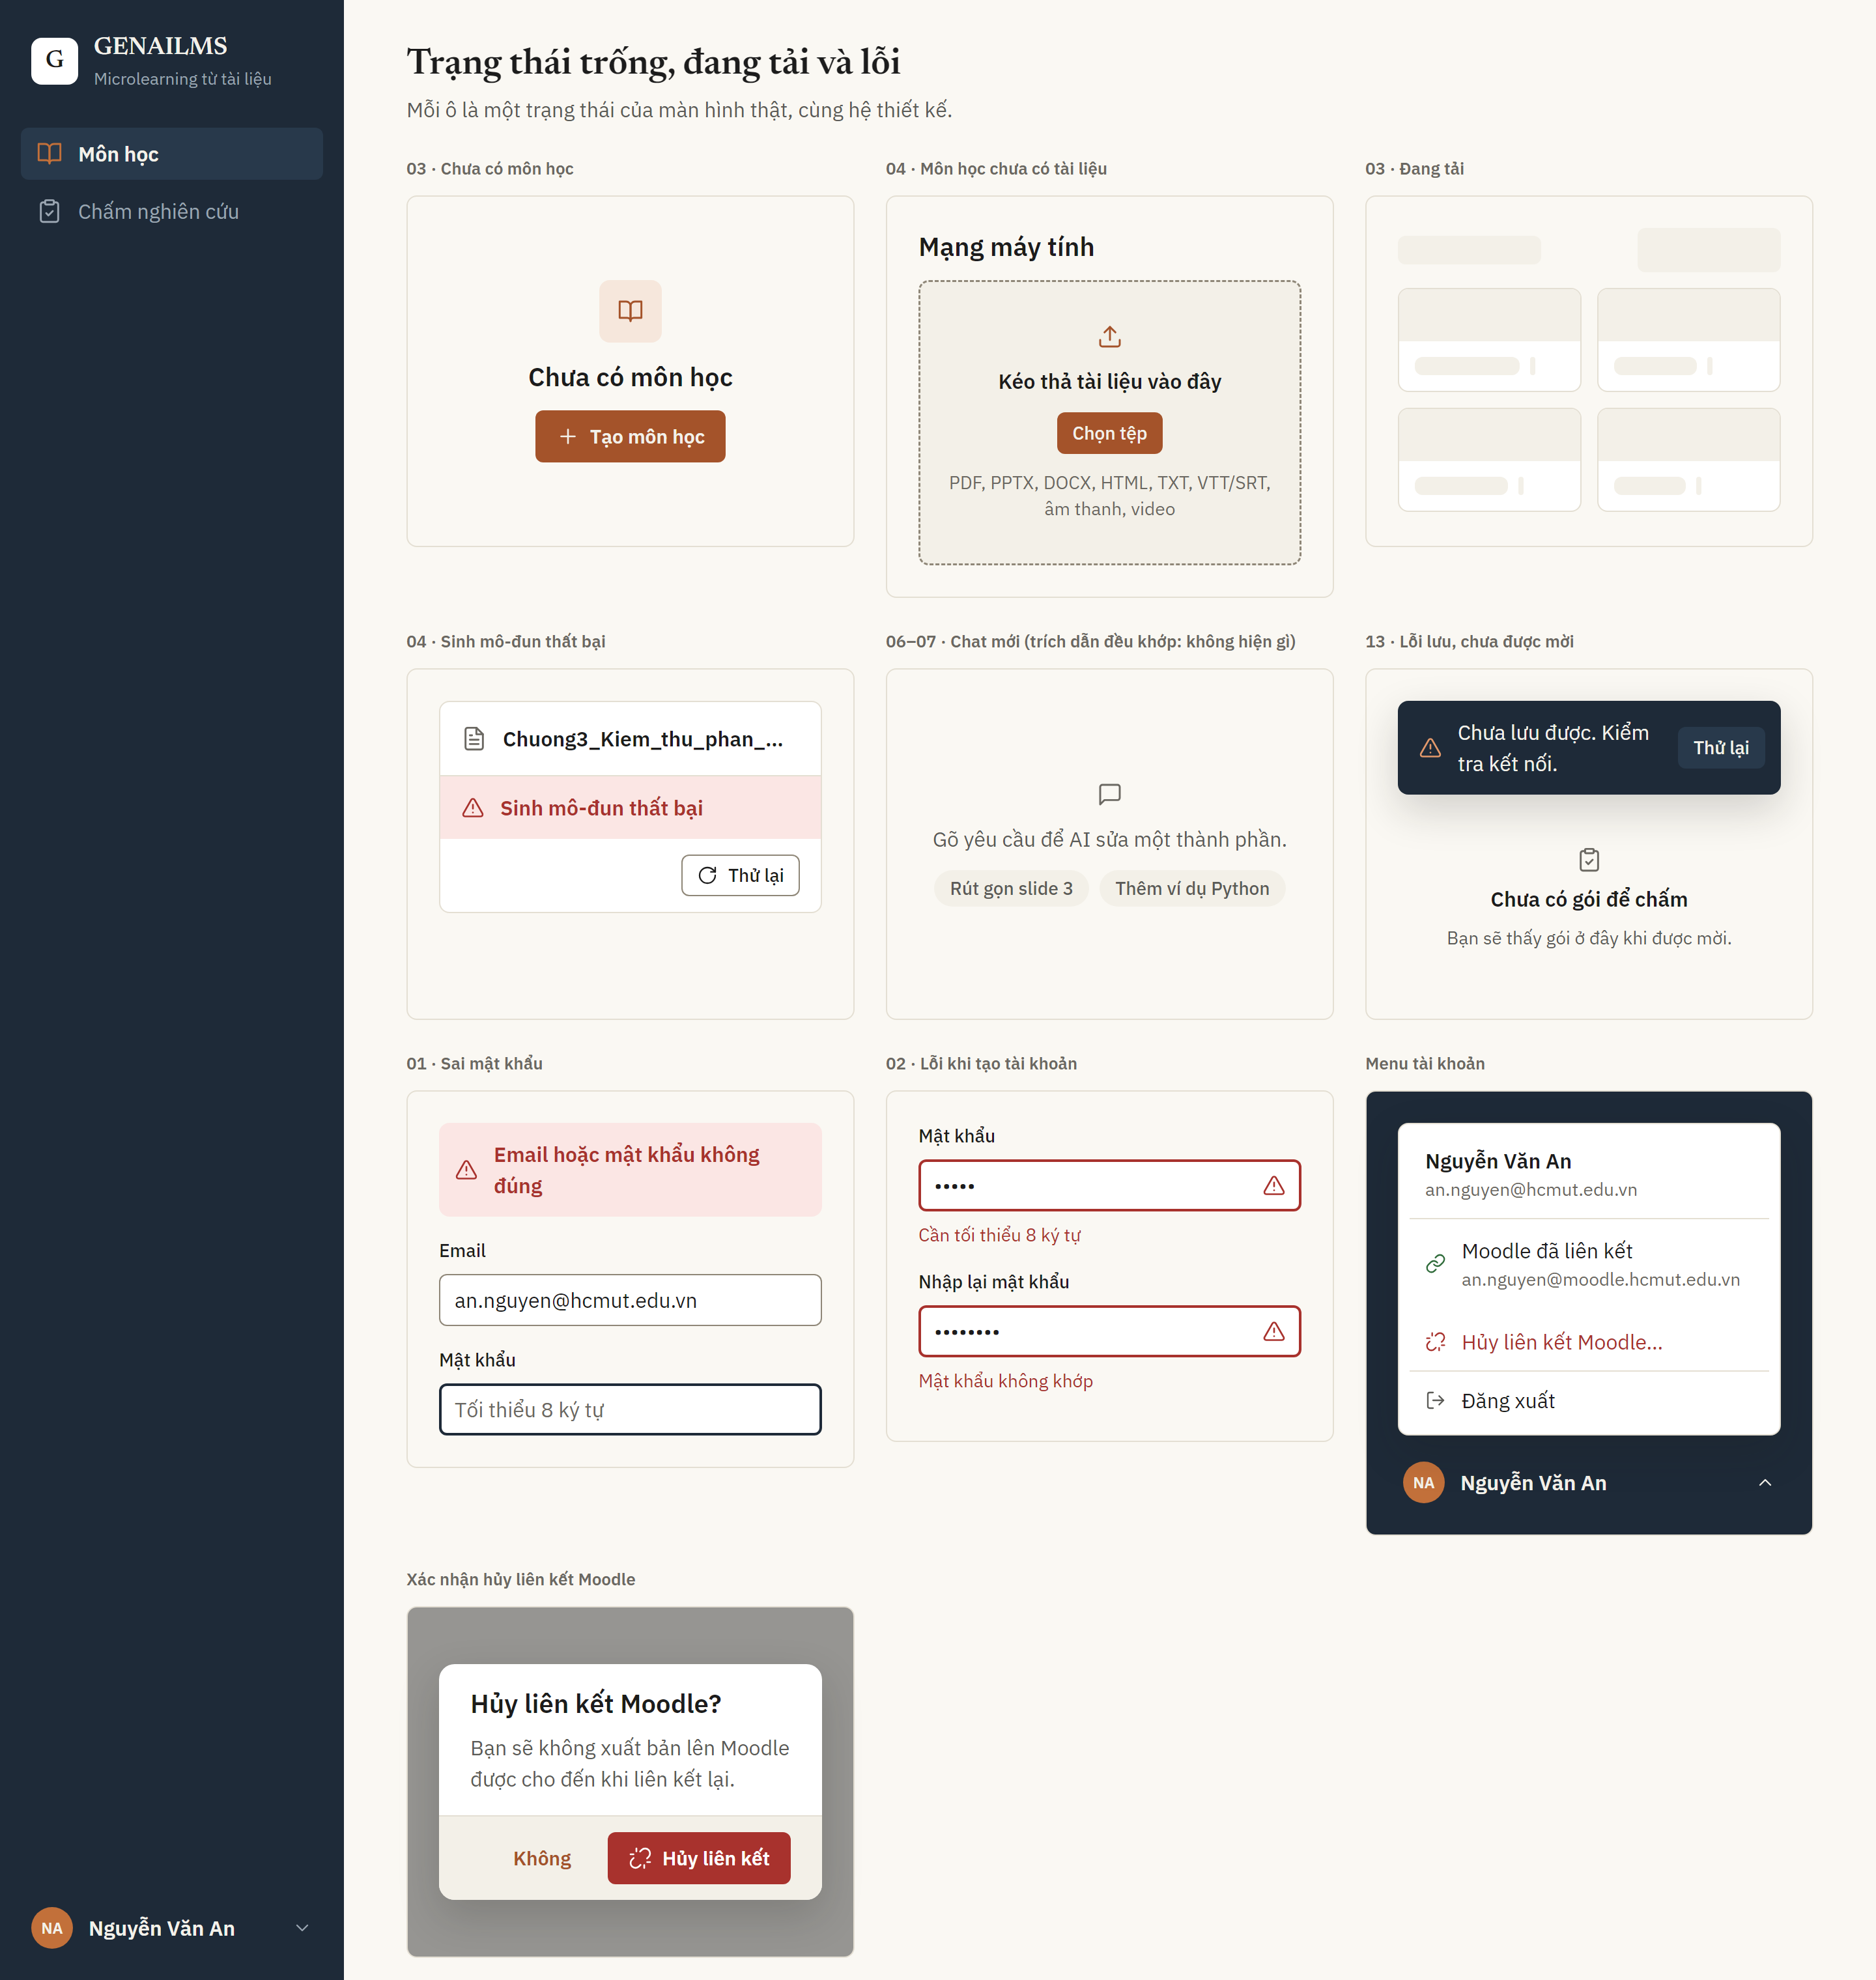
\includegraphics[width=.47\linewidth,height=.26\textheight,keepaspectratio,viewport={620 1480 1320 2000},clip]{graphics/ui/15-empty-loading-error-states.png}\hfill
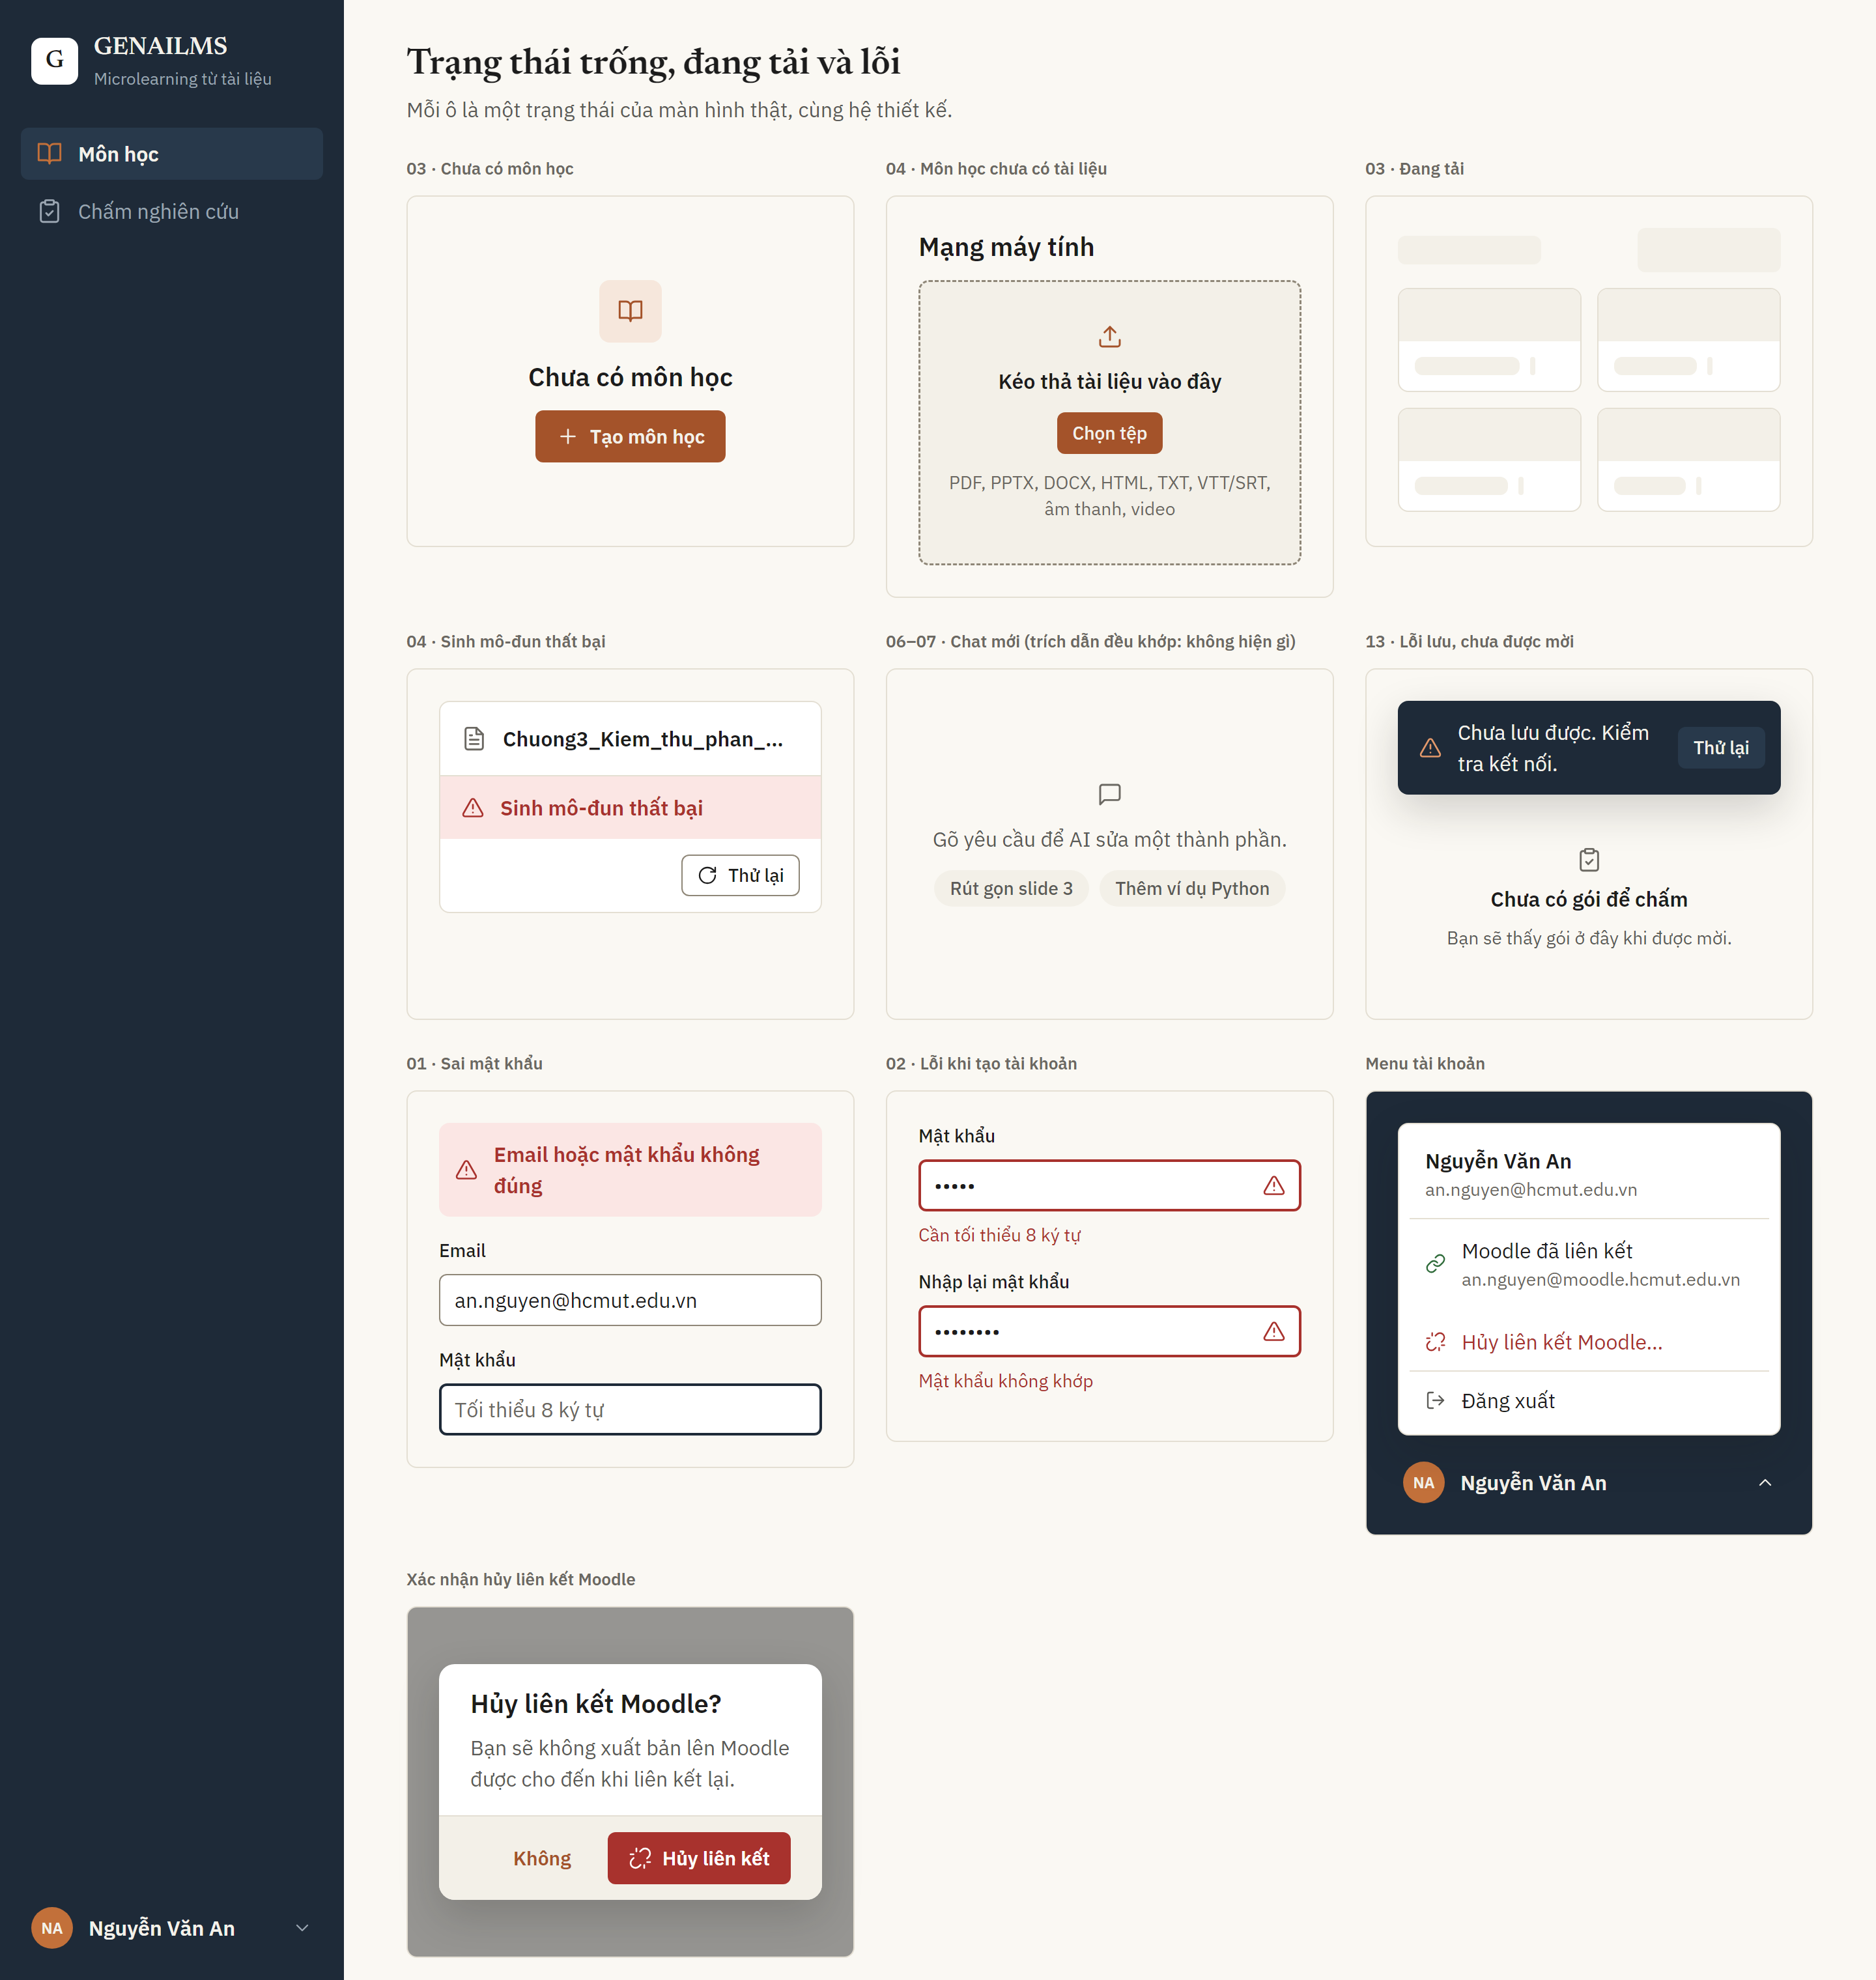
\includegraphics[width=.47\linewidth,height=.26\textheight,keepaspectratio,viewport={1360 1480 2050 2000},clip]{graphics/ui/15-empty-loading-error-states.png}\par\smallskip
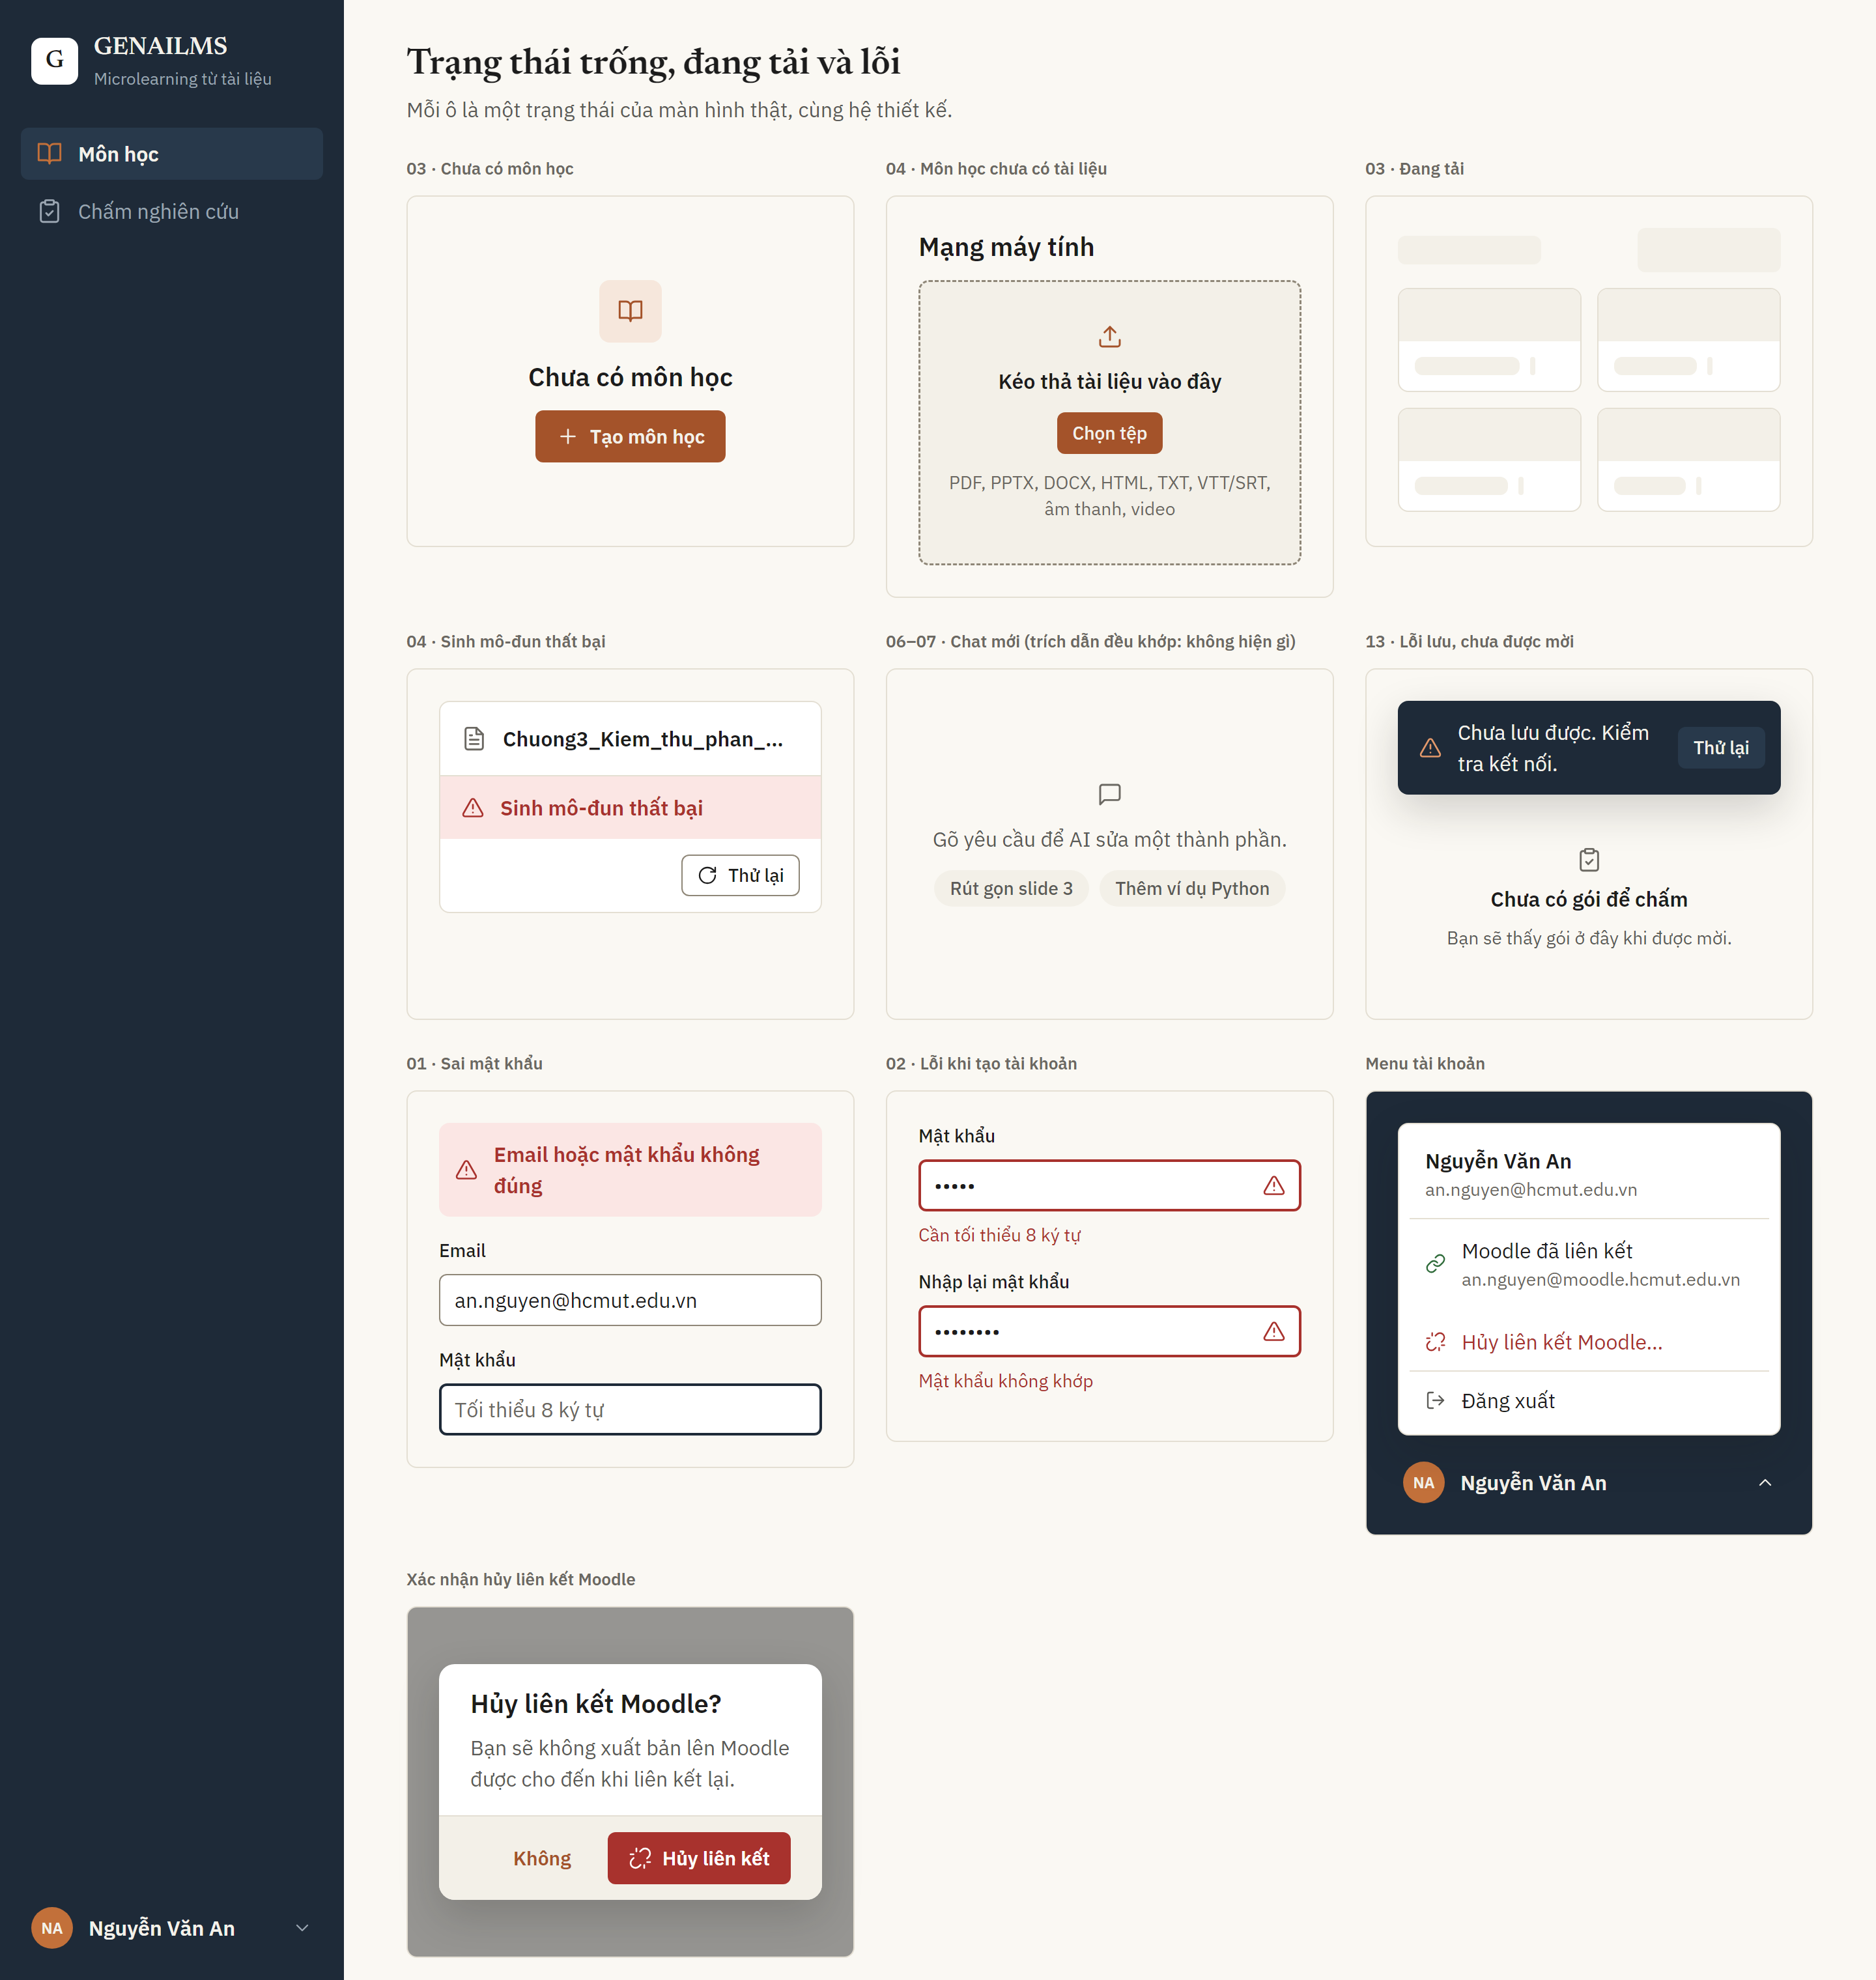
\includegraphics[width=.47\linewidth,height=.26\textheight,keepaspectratio,viewport={2100 1480 2800 2000},clip]{graphics/ui/15-empty-loading-error-states.png}\hfill
\caption{Failure recovery and empty conversation.}\label{fig:ui-screen-15-recovery}
\end{figure}

\needspace{.42\textheight}
Figure~\ref{fig:ui-screen-15-account} enlarges credential validation and account controls. ``Hủy liên kết Moodle'' means ``Unlink Moodle'' and ``Đăng xuất'' means ``Sign out''; unlinking requires confirmation because publication access changes.
\begin{figure}[H]\centering
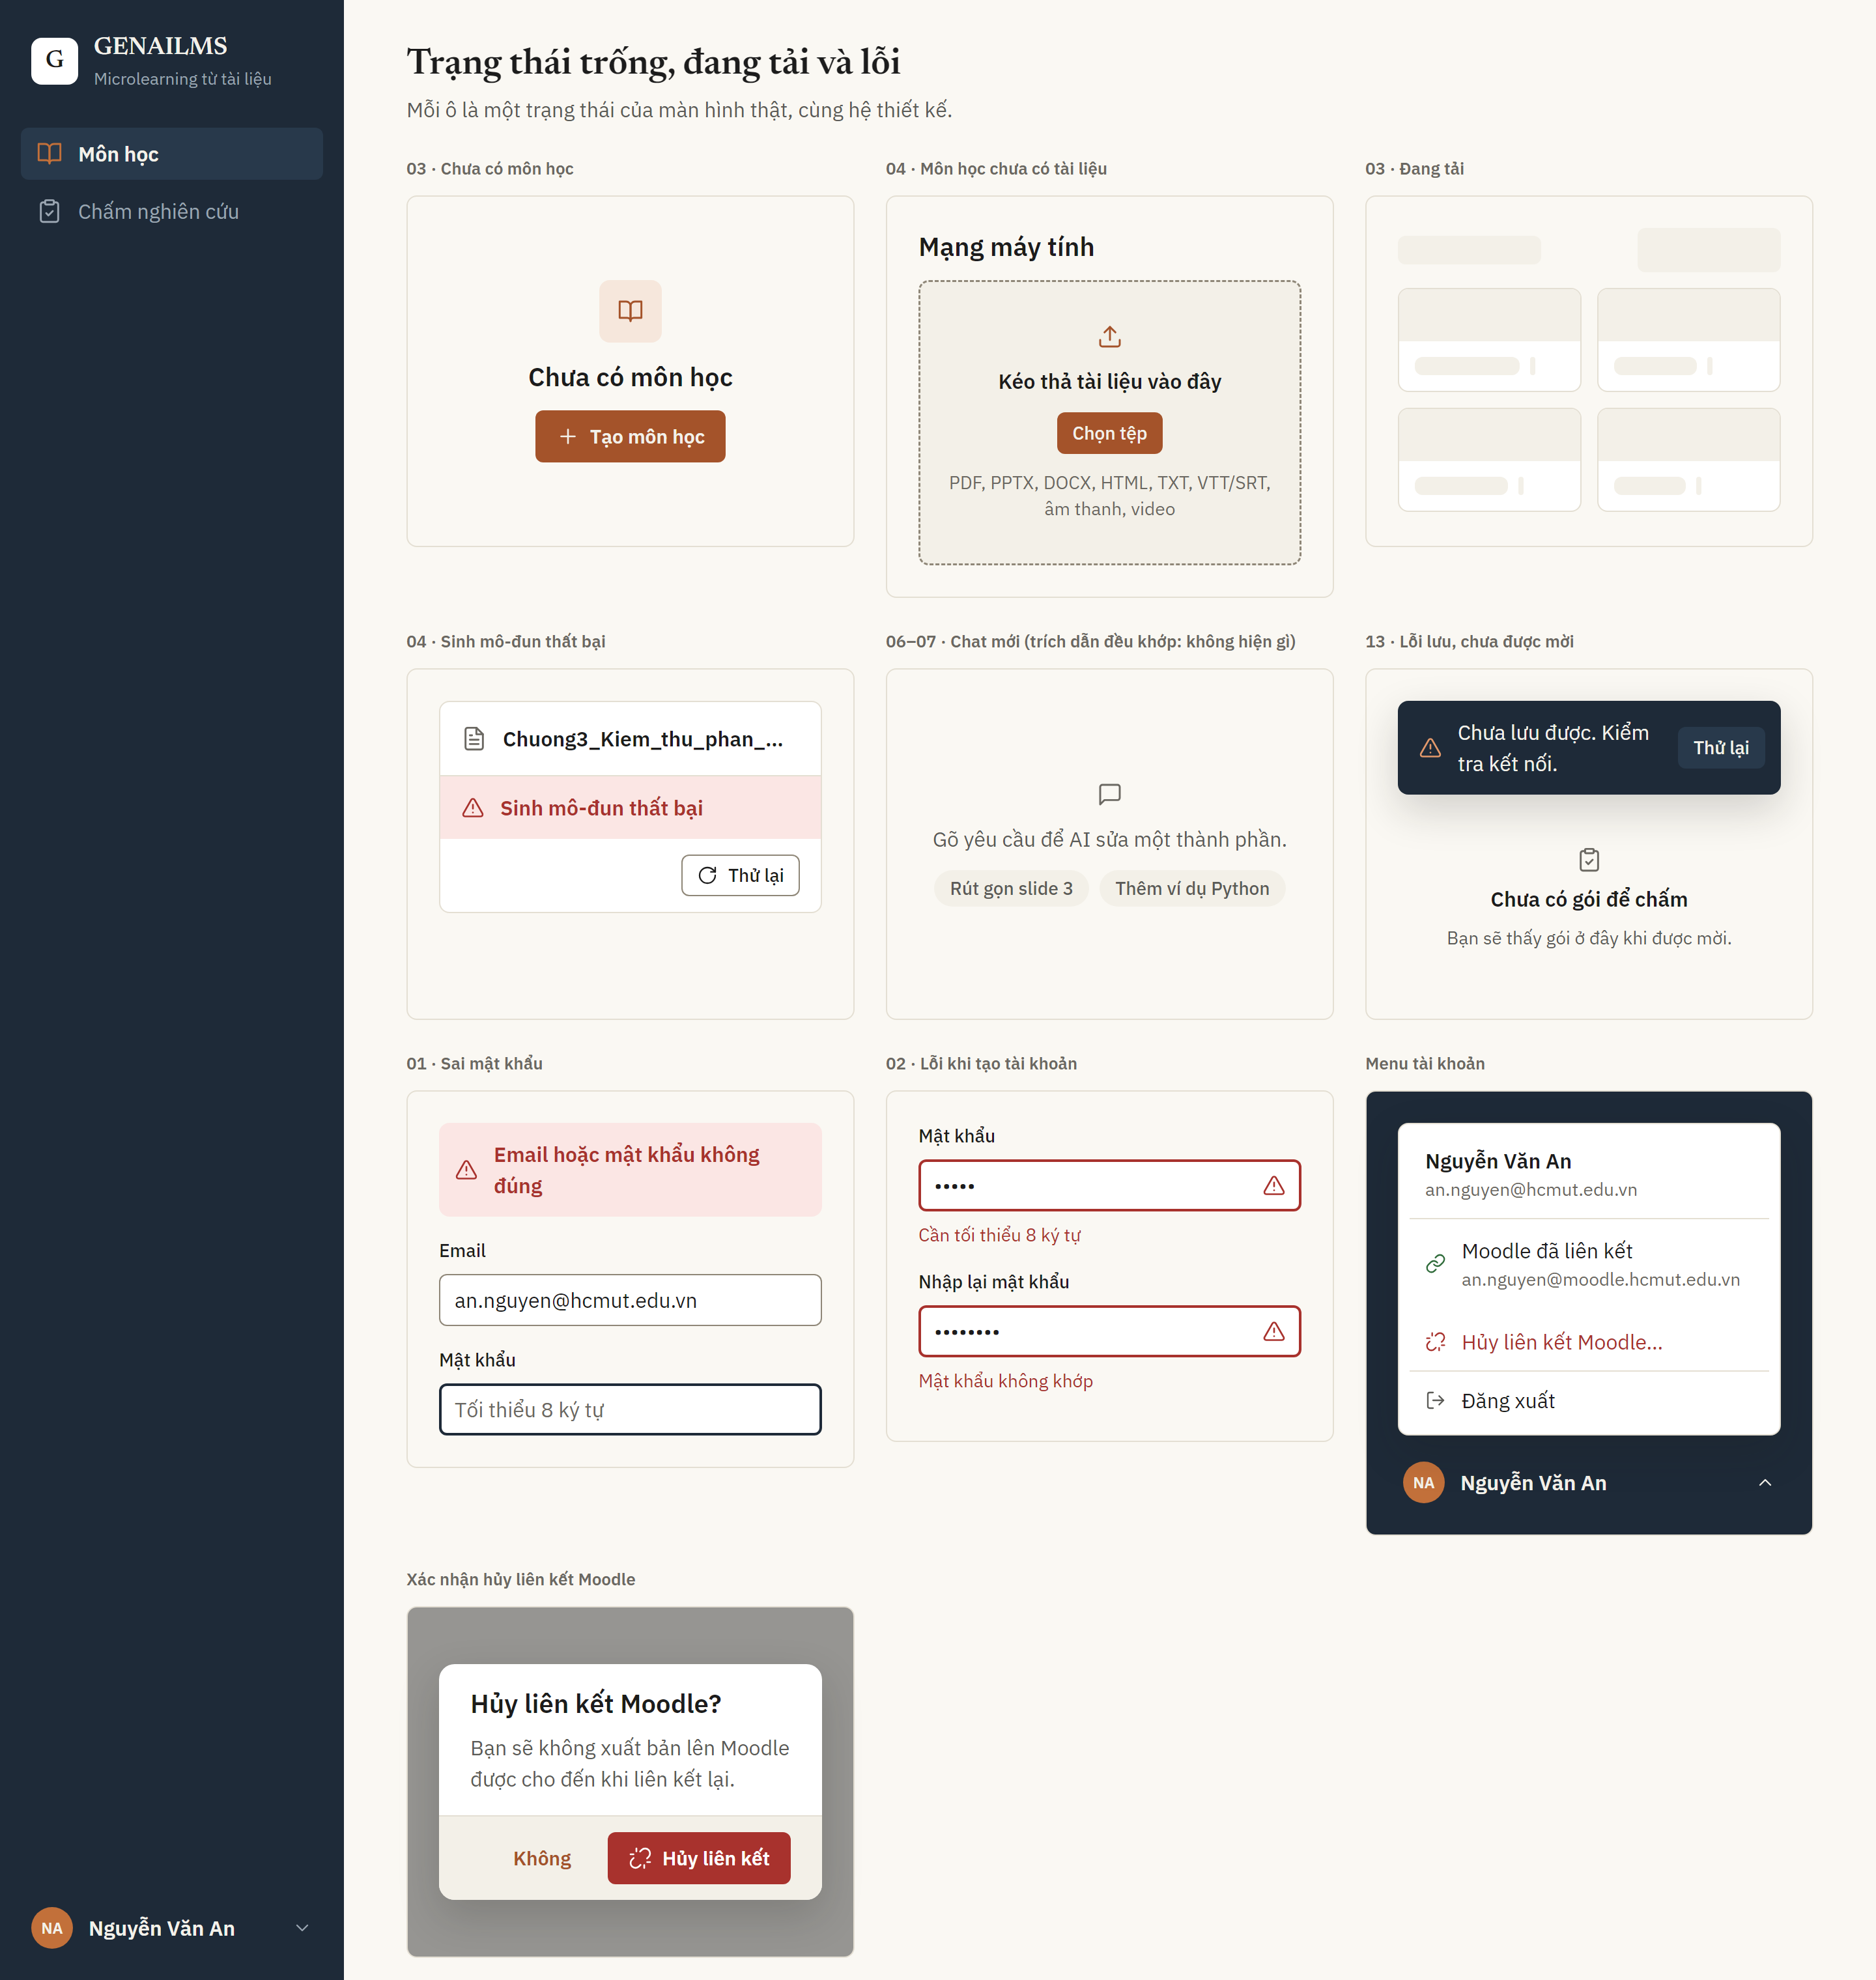
\includegraphics[width=.47\linewidth,height=.26\textheight,keepaspectratio,viewport={620 750 1320 1380},clip]{graphics/ui/15-empty-loading-error-states.png}\hfill
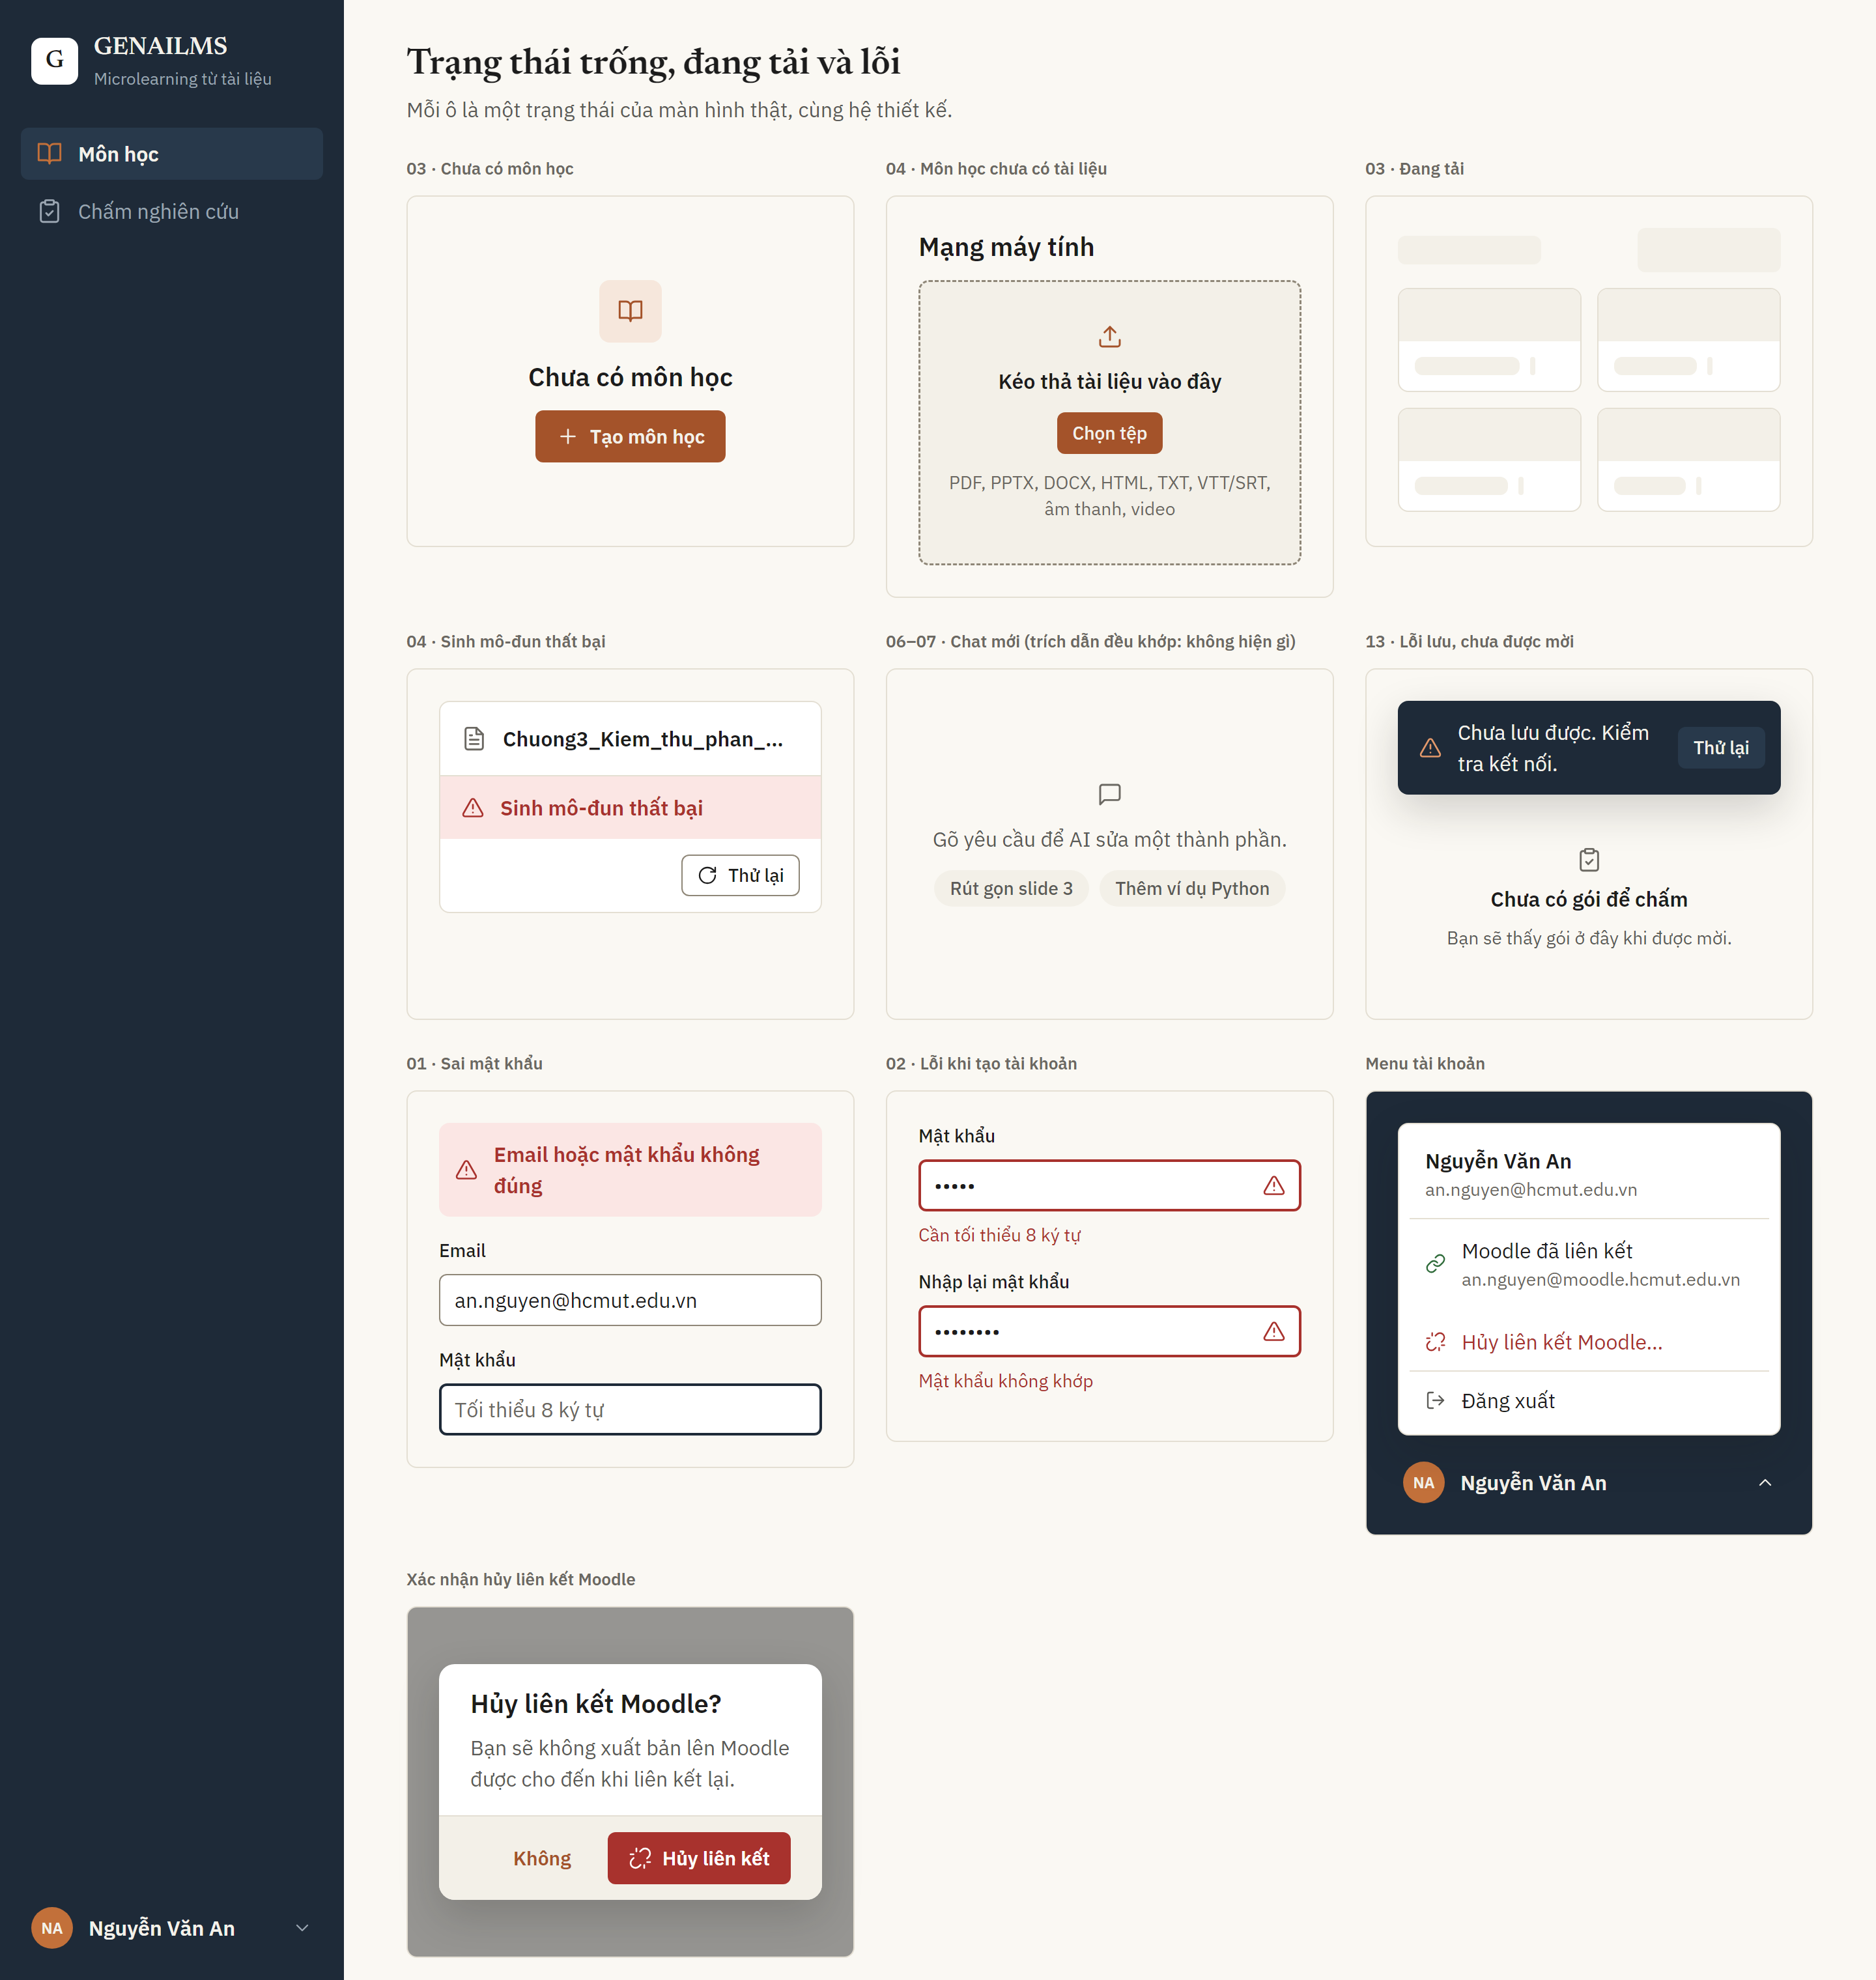
\includegraphics[width=.47\linewidth,height=.26\textheight,keepaspectratio,viewport={1360 790 2050 1380},clip]{graphics/ui/15-empty-loading-error-states.png}\par\smallskip
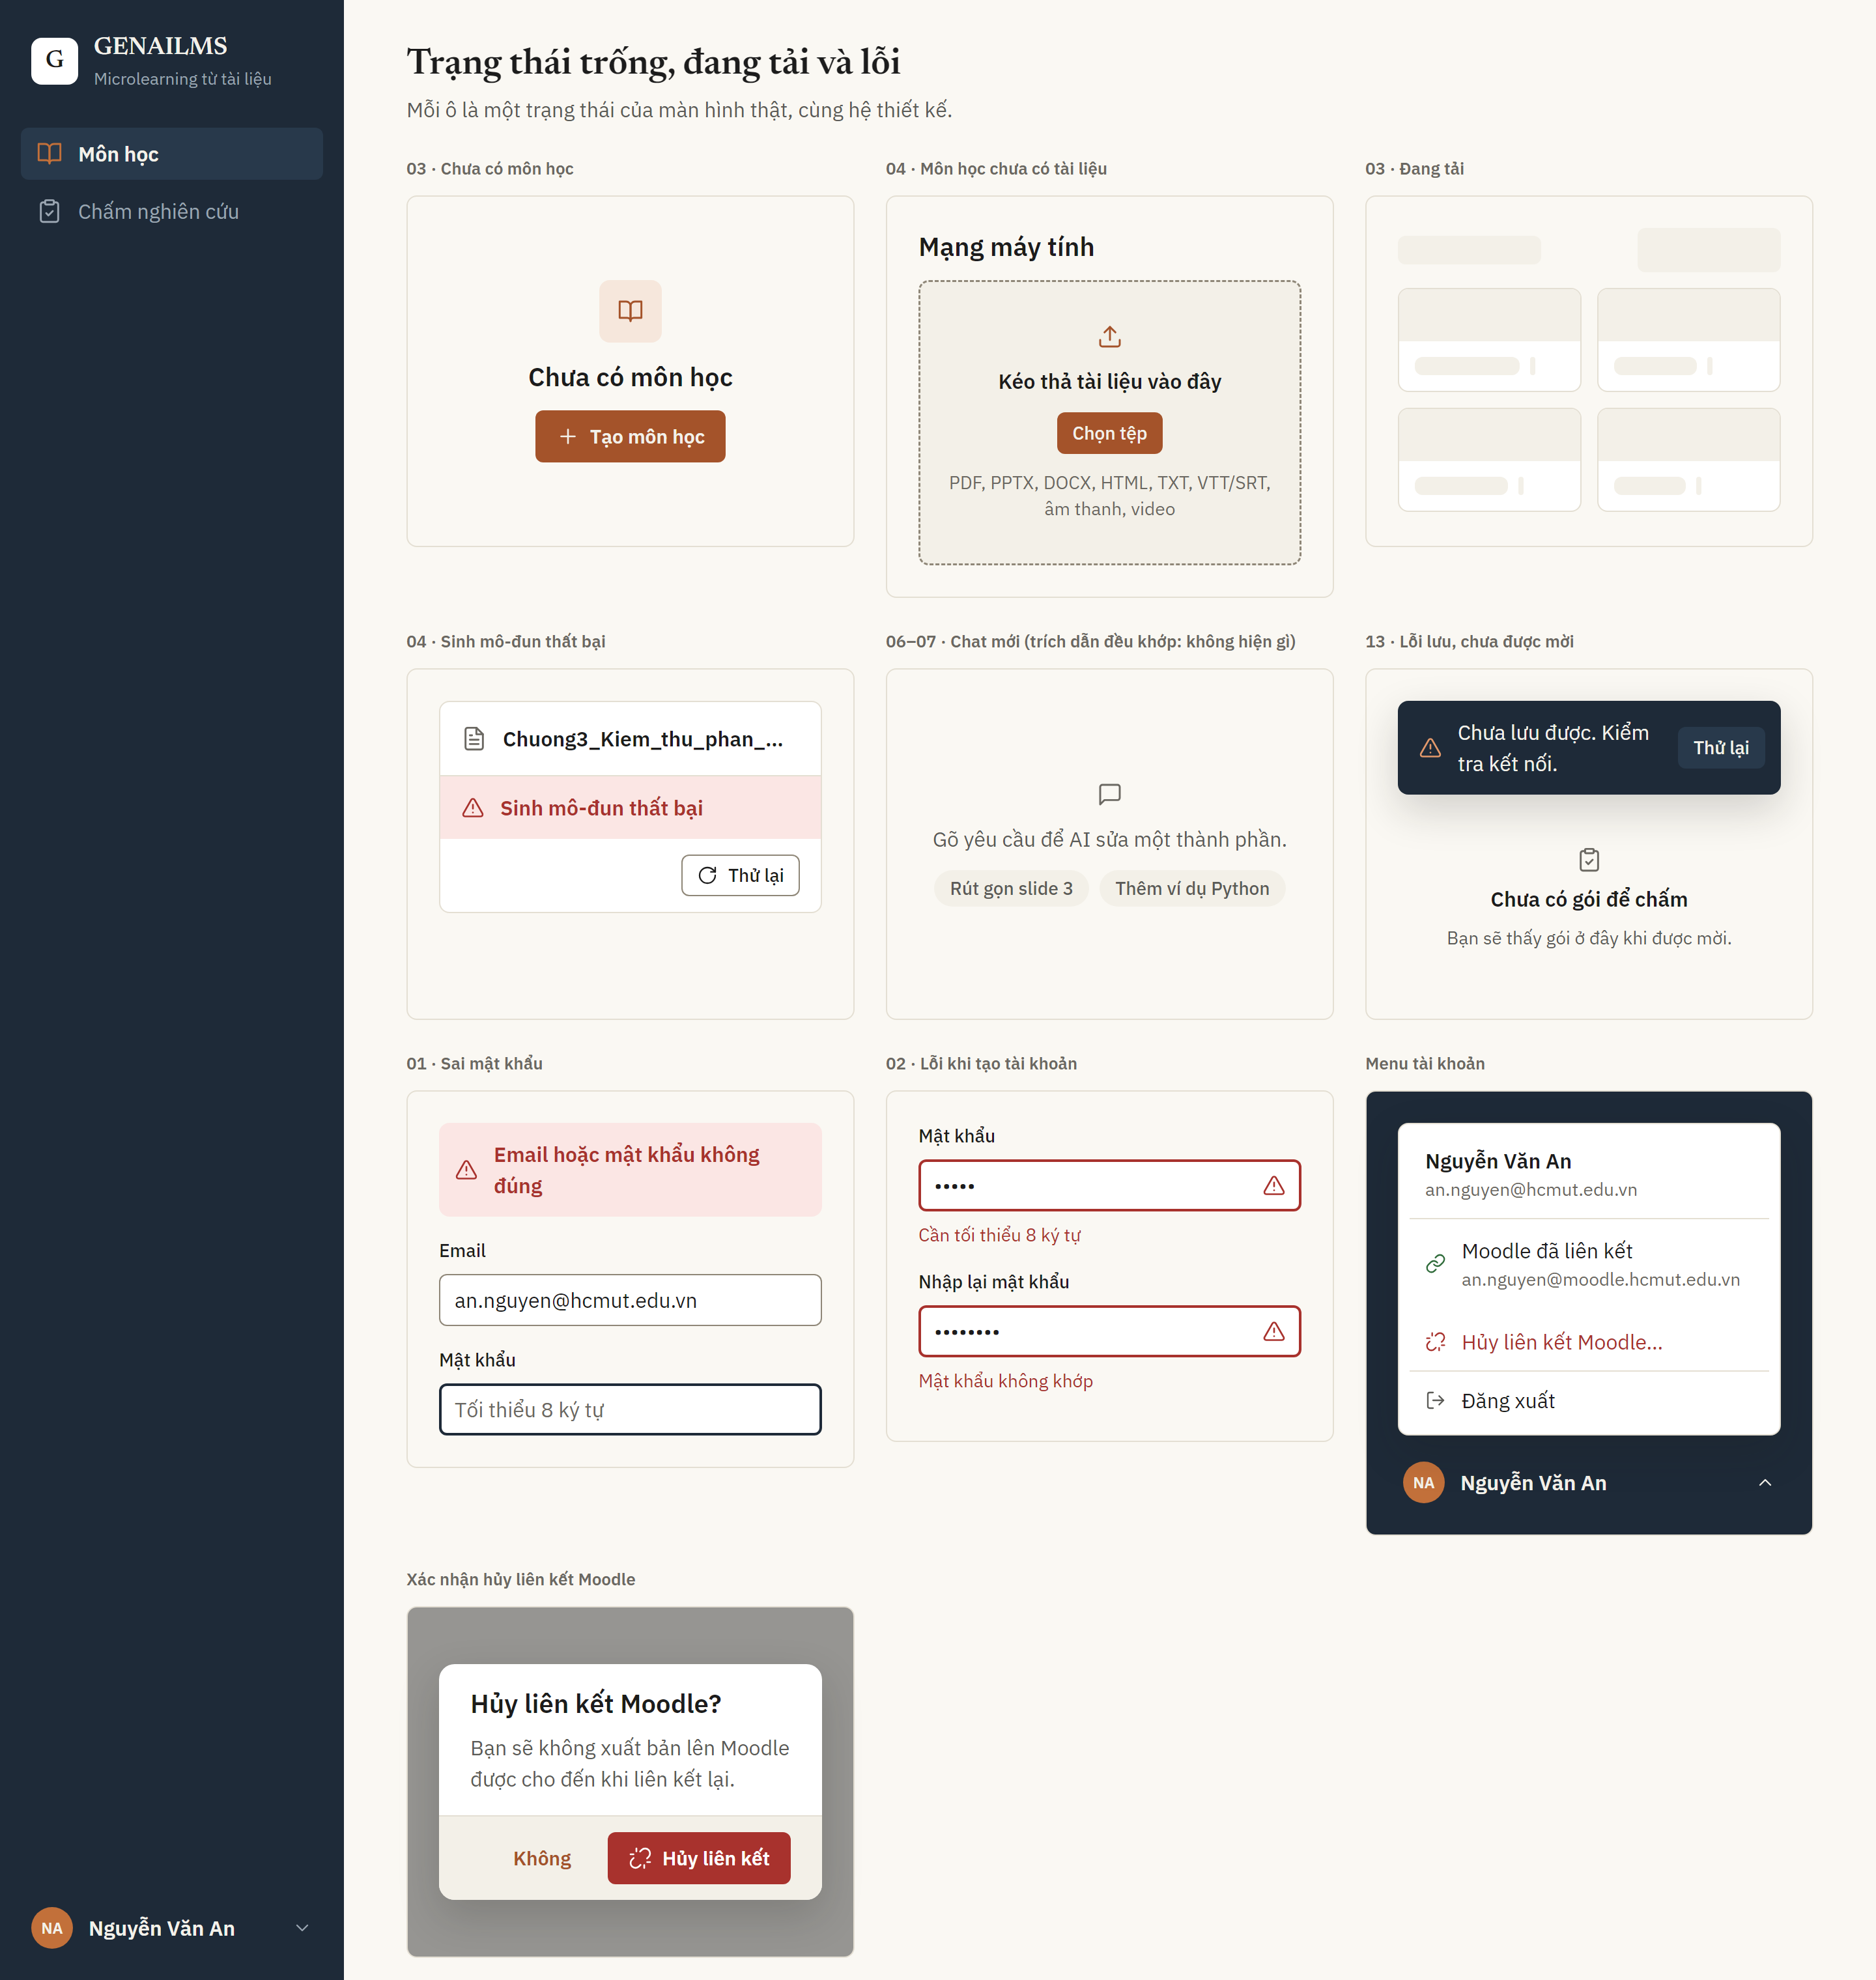
\includegraphics[width=.47\linewidth,height=.26\textheight,keepaspectratio,viewport={2100 640 2800 1380},clip]{graphics/ui/15-empty-loading-error-states.png}\hfill
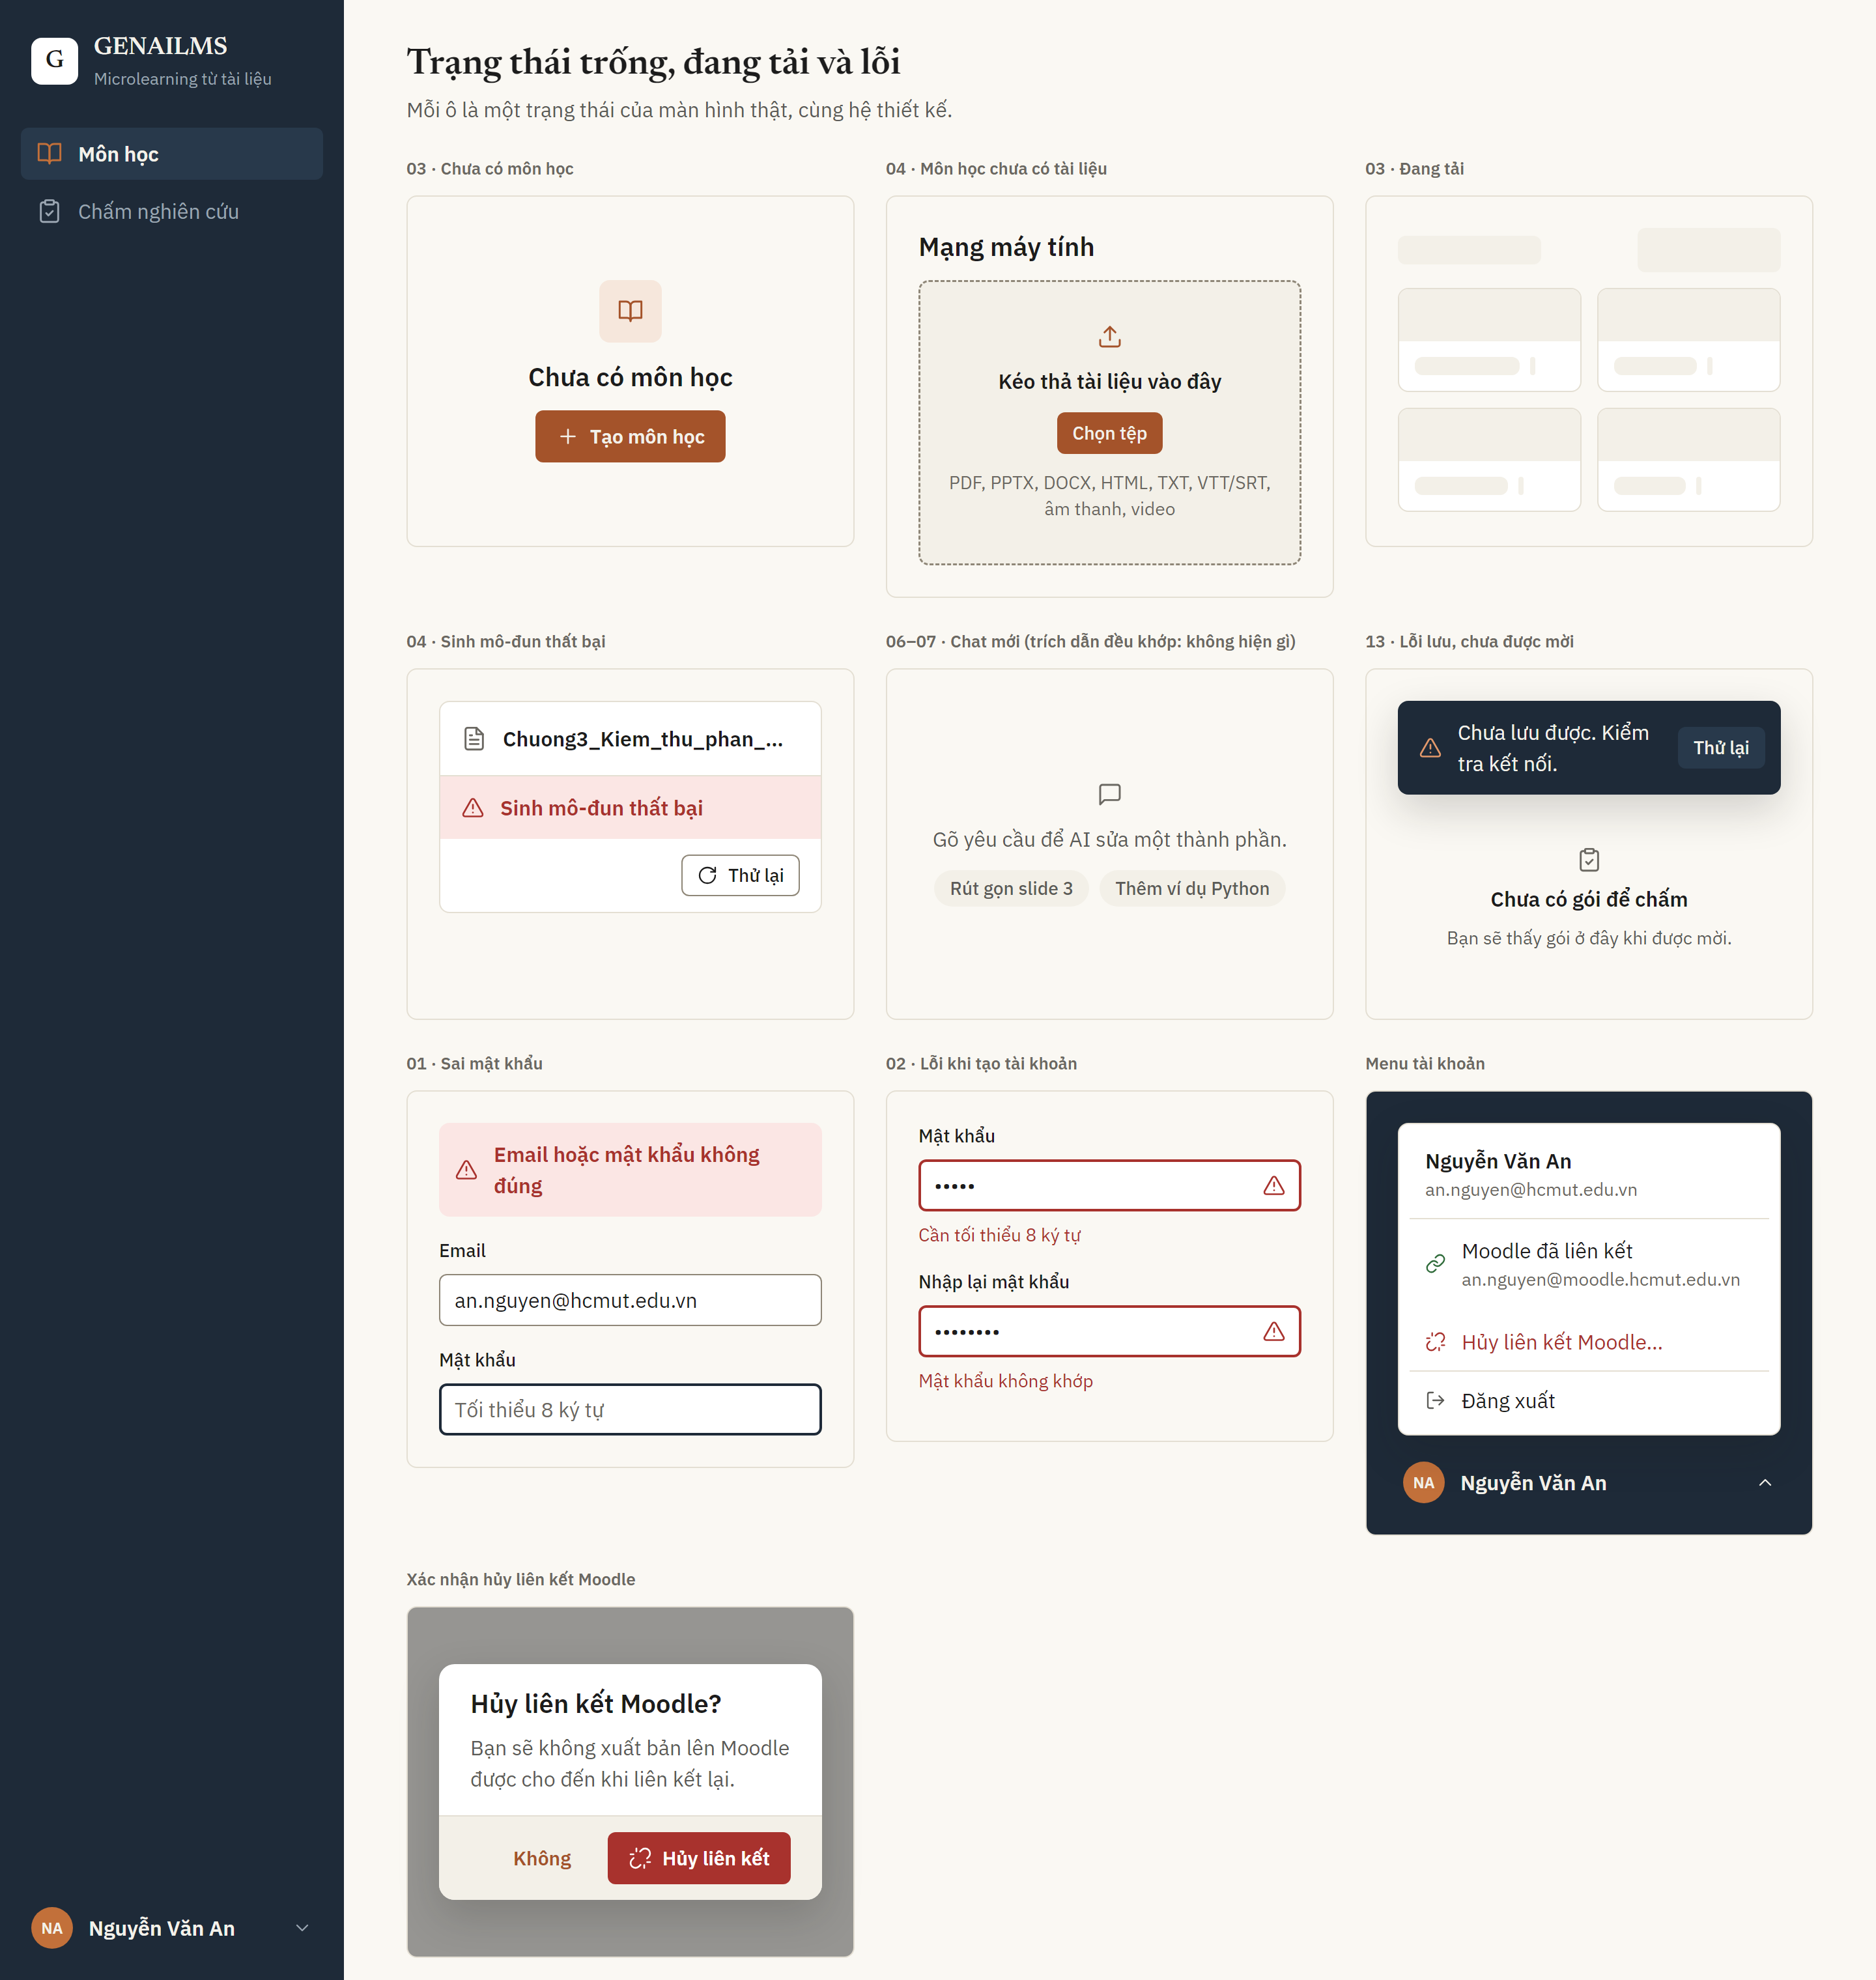
\includegraphics[width=.47\linewidth,height=.26\textheight,keepaspectratio,viewport={620 20 1320 580},clip]{graphics/ui/15-empty-loading-error-states.png}\par\smallskip
\caption{Validation, account menu and unlink confirmation.}\label{fig:ui-screen-15-account}
\end{figure}
